\documentclass[krantz2]{krantz}\usepackage{knitr}

\usepackage{color}

\usepackage{hologo}

\usepackage{csquotes}

\usepackage{graphicx}
\DeclareGraphicsExtensions{.jpg,.pdf,.png}

\usepackage{animate}

\usepackage[style=authoryear-comp,giveninits,sortcites,maxcitenames=2,%
    mincitenames=1,maxbibnames=10,minbibnames=10,backref,uniquename=mininit,%
    uniquelist=minyear,sortgiveninits=true,backend=biber]{biblatex}

\newcommand{\href}[2]{\emph{#2} (\url{#1})}

\usepackage{framed}

\usepackage{abbrev}
\usepackage{usingr}

\usepackage{imakeidx}

% this is to reduce spacing above and below verbatim, which is used by knitr
% to show returned values
\usepackage{etoolbox}
\makeatletter
\preto{\@verbatim}{\topsep=-5pt \partopsep=-4pt \itemsep=-2pt}
\makeatother

% for drawing flowcharts
\usepackage{tikz}
\usetikzlibrary{shapes.geometric,positioning,fit,arrows}
\tikzstyle{startstop} = [rectangle, rounded corners, minimum width=3cm, minimum height=1cm,text centered, draw=black]
\tikzstyle{io} = [trapezium, trapezium left angle=70, trapezium right angle=110, minimum width=3cm, minimum height=1cm, text centered, draw=black]
\tikzstyle{process} = [rectangle, minimum width=3cm, minimum height=1cm, text centered, draw=black]
%tight boxes
\tikzstyle{tprocess} = [rectangle, minimum width=2cm, minimum height=0.66cm, text centered, draw=black]
\tikzstyle{enclosure} = [rectangle, minimum width=3.4cm, minimum height=3cm, text centered, draw=black]
\tikzstyle{decision} = [diamond, aspect=2, minimum width=3cm, minimum height=1cm, text centered, draw=black]
\tikzstyle{arrow} = [thick,->,>=latex]

\tikzset{
 a/.style
  = {node distance=4em, text width=0.1em, minimum height=4em},
 b/.style
  = {rectangle, draw, fill=gray!10, node distance=4em, text width=6em,
     text centered, rounded corners, minimum height=4em, thick},
 c/.style
  = {circle, draw, dashed, fill=orange!10, inner sep = 0pt, node distance=4em, text width=6em,
     text centered, thick},
 cc/.style
  = {circle, draw, dashed, fill=orange!10, inner sep = 0pt, node distance=4em, text width=3em,
     text centered, thick},
 l/.style
  = {draw, -latex, ultra thick},
 aa/.style
  = {node distance=4em, text width=0em, minimum height=0.5ex},
 ll/.style
  = {draw, {open triangle 45} -, thick},
}

%\usepackage{polyglossia}
%\setdefaultlanguage{english}

\setcounter{topnumber}{3}
\setcounter{bottomnumber}{3}
\setcounter{totalnumber}{4}
\renewcommand{\topfraction}{0.90}
\renewcommand{\bottomfraction}{0.90}
\renewcommand{\textfraction}{0.10}
\renewcommand{\floatpagefraction}{0.70}
\renewcommand{\dbltopfraction}{0.90}
\renewcommand{\dblfloatpagefraction}{0.70}

% ensure page numbers are aligned in TOC
\makeatletter
\renewcommand{\@pnumwidth}{2.05em}
\makeatother

\addbibresource{rbooks.bib}
\addbibresource{references.bib}

\makeindex[title=General index]
\makeindex[name=rindex,title=Alphabetic index of \Rlang names]
\makeindex[name=rcatsidx,title=Index of \Rlang names by category]
\makeindex[name=cloudindex]
\IfFileExists{upquote.sty}{\usepackage{upquote}}{}
\begin{document}
\hyphenation{pro-cess-ing paren-the-ses spe-cif-ic au-thors in-ter-act-ed lim-it}

\title{\Huge{\fontseries{ub}\sffamily Learn R\\{\Large As a Language}}}

\author{Pedro J. Aphalo}

\date{Helsinki, \today}

% knitr setup

















\frontmatter

\maketitle

\newpage

\setcounter{page}{5} %previous pages will be reserved for frontmatter to be added in later.
\tableofcontents
\listoffigures



%\include{frontmatter/foreword}
%\chapter*{Preface}

\begin{VF}
``Suppose that you want to teach the `cat' concept to a very young child. Do you explain that a cat is a relatively small, primarily carnivorous mammal with retractible claws, a distinctive sonic output, etc.? I'll bet not. You probably show the kid a lot of different cats, saying `kitty' each time, until it gets the idea. To put it more generally, generalizations are best made by abstraction from experience.''

\VA{R. P. Boas}{Can we make mathematics intelligible?}
\end{VF}

%\dictum[R. P. Boas (1981) Can we make mathematics intelligible?, \emph{American Mathematical Monthly} \textbf{88:} 727-731.]{"Suppose that you want to teach the `cat' concept to a very young child. Do you explain that a cat is a relatively small, primarily carnivorous mammal with retractible claws, a distinctive sonic output, etc.? I'll bet not. You probably show the kid a lot of different cats, saying `kitty' each time, until it gets the idea. To put it more generally, generalizations are best made by abstraction from experience."}


% Such pauses are not a miss use of our time. To learn a natural language we need to interact with other speakers, we need feedback. In the case of R, we can get feedback both from the outcomes from our utterances to the computer, and from other \Rlang users.}
\noindent
This book covers different aspects of the use of the \Rlang language. Chapters \ref{chap:R:introduction} to \ref{chap:R:functions} describe the \Rlang language itself. Later chapters describe extensions to the \Rlang language available through contributed \emph{packages}, the \emph{grammar of data} and the \emph{grammar of graphics}. In this book, explanations are concise but contain pointers to additional sources of information, so as to encourage the development of a routine of independent exploration. This is not an arbitrary decision, this is the normal \emph{modus operandi} of most of us who use \Rlang regularly for a variety of different problems. Some have called approaches like the one used here ``learning the hard way'', but I would call it ``learning to be independent''.

I do not discuss statistics or data analysis methods in this book, I describe \Rlang as a language for data manipulation and display. The idea is for you to learn the \Rlang language in a way comparable to how children learn a language: they work out what the rules are, simply by listening to people speak and trying to utter what they want to tell their parents. Of course, small children receive some guidance, but they are not taught a prescriptive set of rules like when learning a second language at school. Instead of listening, you will read code and instead of speaking you will try to execute \Rlang  code statements on a computer---i.e. you will try your hand at using \Rlang to tell a computer what you want it to compute. I do provide explanations and guidance, but the idea of this book is for you to use the numerous examples to find out by yourself the overall patterns and coding philosophy behind the \Rlang language. Instead of parents being the sound board for your first utterances in \Rlang, the computer will play this role. You will \emph{play} by modifying the examples, see how the computer responds: does \Rlang understand you or not? Using a language actively is the most efficient way of learning it. By using it, I mean actually reading, writing and running scripts or programs (copying and pasting, or typing ready-made examples from books or the internet does not qualify as using a language).

I have been using \Rlang since around 1998 or 1999, but I am still constantly learning new things about \Rlang itself and \Rlang packages. With time it has replaced in my work as a researcher and teacher several other pieces of software: \pgrmnameNI{SPSS}, \pgrmnameNI{Systat}, \pgrmnameNI{Origin}, \pgrmnameNI{MS-Excel}, and it has become a central piece of the tool set I use for producing lecture slides, notes, books and even web pages. This is to say that it is the most useful piece of software and programming language I have ever learnt to use. Of course, in time it will be replaced by something better, but at the moment it is a key language to learn for anybody with a need to analyse and display data.

What is a language? A language is a system of communication. \Rlang as a language allows us to communicate with other members of the \Rlang community, and with computers. As all languages in active use, \Rlang evolves. New ``words'' and new ``constructs'' are incorporated into the language, and some earlier frequently used ones are relegated to the fringes of the corpus. I describe current usage and ``modisms'' of the \Rlang language in a way accessible to a readership unfamiliar with computer science but with some background in data analysis as used in Biology, Engineering, or Humanities.

When teaching I tend to lean towards challenging students rather than telling an over-simplified story. There are two reasons for this. First, I prefer as a student, and I learn best myself if the going is not too easy. Second, if I would hide the tricky bits of the \Rlang language, it would make readers' life much more difficult later on. You will not remember all the details, nobody could. However, you most likely will remember or develop a sense of in which situations you need to be careful or should check the details. So, I will expose you not only the usual cases, but also to several exceptions and counterintuitive features of the language, which I have highlighted with icons. Reading this book will be about exploring a new world; this book aims to be a travel guide, but neither a traveler's account, nor a cookbook of \Rlang recipes.

Keep in mind that it is impossible to remember everything about \Rlang! The \Rlang language in a broad sense is vast because its capabilities can be expanded with independently developed packages. Learning to use \Rlang consists in learning the basics plus developing the skill of finding your way in \Rlang and its documentation.  In 2017 the number packages available in the Comprehensive \Rlang Archive Network (CRAN) broke the 10\,000 barrier. CRAN is the most important, but not only, public repository for \Rlang packages. How good a command of the \Rlang language and packages a user needs depends on the type of activities to be carried out. This book attempts to train you in the use of the \Rlang language itself and of popular \Rlang language extensions for data manipulation and graphical display. Given the availability of numerous books on statistical analysis with \Rlang, in the present book I will cover only the bare minimum of this subject. The same is true for package development in \Rlang. This book seats in-between, aiming at teaching programming in-the-small: the use of \Rlang to automate the drudgery of data manipulation from raw data, through data exploration to the production of publication quality illustrations.

As with all ``rich'' languages there are many different ways of doing things in \Rlang, and there is in almost all cases no one-size-fits-all solution to a problem. There is always a compromise involved, usually between time spent by the user and processing time required in the computer. Many of the packages that are most popular nowadays did not exist when I started using \Rlang, and many of these packages make new approaches available. One could write many different \Rlang books with a given aim using substantially different ways of achieving the same results. In this book, I limit myself to packages that are currently popular and/or that I consider elegantly designed. I have in particular tried to limit myself to packages with similar design philosophies, especially in relation to their interfaces. What is elegant design, and in particular what is a friendly user interface depends strongly on each user's preferences and previous experience. Consequently, the contents of the book are strongly biased by my own preferences. I have tried to write examples in ways that execute fast without compromising readability. I encourage readers to take this book as a starting point for exploring the very many packages, styles and approaches which I have not described.

I will appreciate suggestions for further examples, notification of errors and unclear sections. Many of the examples here have been collected from diverse sources over many years and because of this not all sources are acknowledged. If you recognize any example as yours or someone else's please let me know so that I can add a proper acknowledgement. I warmly thank the students that over the years have asked the questions and posed the problems that have helped me write this text and correct the mistakes and voids of previous versions. I have also received help on on-line forums and in person from numerous people, learnt from archived e-mail list messages, blog posts, books, articles, tutorials, webinars, and by struggling to solve some new problems on my own. In many ways this text owes much more to people who are not authors than to myself. However, as I am the one who has written this version and decided what to include and exclude, as author, I take full responsibility for any errors and inaccuracies.

Why have I chosen the title ``\emph{Learn R \ldots as you learnt your mother tongue}''? On one hand, because this book is based on exploration and practice. On the other hand, because you will be exposed to current usage and not spared the quirks of the language. When we use our mother tongue in everyday life we do not think about grammar rules or sentence structure, except for the trickier or unfamiliar situations. My aim is for this book to help you grow to use \Rlang in this same way, to become fluent in \Rlang. The book is structured around the elements of languages with chapter titles that highlight the parallels between natural languages like English and the \Rlang language.

\emph{I encourage you to approach \Rlang, like a child approaches his or hers mother tongue when first learning to speak: Do not struggle, just play, fool around with \Rlang! If going gets difficult and frustrating, take a break! If you get a new insight, take a break to enjoy the victory!
}%\end{framed}

\newpage
%\vfill
%\begin{framed}
\noindent
\section*{Icons used to mark different content}

Text boxes are used throughout the book to highlight content that plays specific roles in the learning process or that require special attention from the reader. Each box contains one of five different icons that indicate the type of its contents as described below.\\[1.5ex]

\noindent
\playicon\ Signals \emph{playground} boxes which contain open-ended exercises---ideas and pieces of \Rlang code to play with at the \Rlang console.\\[1.5ex]

\noindent
\advplayicon\ Signals \emph{advanced playground} which will require more time to play with before grasping concepts than regular \emph{playground} boxes.\\[1.5ex]

\noindent
\ilAttention\ Signals important bits of information that must be remembered when using \Rlang---i.e.\ explain some unusual feature of the language.\\[1.5ex]

\noindent
\ilAdvanced\ Signals in-depth explanations of specific points that may require you to spend time thinking, which en general can be skipped on first reading, but to which you should return at a later, peaceful, time preferably with a cup of coffee or tea.\\[1.5ex]

\noindent
\infoicon\ Signals text boxes providing general information not directly related to the \Rlang language.\\[1.5ex]
%\end{framed}
%\newpage

%\newpage
%\begin{infobox}
%\noindent
%\textbf{Status as of 2016-11-23.} I have updated the manuscript to track package updates since the previous version uploaded six months ago, and added several examples of the new functionality added to packages \ggpmisc, \ggrepel, and \ggplot. I have written new sections on packages \viridis, \pkgname{gganimate}, \pkgname{ggstance}, \pkgname{ggbiplot}, \pkgname{ggforce}, \pkgname{ggtern} and \pkgname{ggalt}. Some of these sections are to be expanded, and additional sections are planned for other recently released packages.
%
%With respect to the chapter \textit{Storing and manipulating data with R} I have put it on hold, except for the introduction, until I can see a soon to be published book covering the same subject. Hadley Wickham has named the set of tools developed by him and his collaborators as \textit{tidyverse} to be described in the book titled \textit{R for Data Science} by Grolemund and Wickham (O'Reilly).
%
%An important update to \ggplot was released last week, and it includes changes to the behavior of some existing functions, specially faceting has become extensible through other packages. Several of the new facilities are described in the updated text and code included in this book and this pdf has been generated with up-to-date version of \ggplot and packages as available today from CRAN, except for \pkgname{ggtern} which was downloaded from Bitbucket minutes ago.
%
%The present update adds about 100 pages to the previous versions. I expect to upload a new update to this manuscript in one or two months time.
%
%\textbf{Status as of 2017-01-17.} Added ``playground'' exercises to the chapter describing \ggplot, and converted some of the examples earlier part of the main text into these playground items. Added icons to help readers quickly distinguish playground sections (\textcolor{blue}{\noticestd{"0055}}), information sections (\textcolor{blue}{\modpicts{"003D}}), warnings about things one needs to be specially aware of (\colorbox{yellow}{\typicons{"E136}}) and boxes with more advanced content that may require longer time/more effort to grasp (\typicons{"E04E}). Added to the sections \code{scales} and examples in the \ggplot chapter details about the use of colors in \Rlang and \ggplot2. Removed some redundant examples, and updated the section on \code{plotmath}. Added terms to the alphabetical index. Increased line-spacing to avoid uneven spacing with inline code bits.
%
%\textbf{Status as of 2017-02-09.} Wrote section on ggplot2 themes, and on using system- and Google fonts in ggpplots with the help of package \pkgname{showtext}. Expanded section on \ggplot's \code{annotation}, and revised some sections in the ``R scripts and Programming'' chapter. Started writing the data chapter. Wrote draft on writing and reading text files. Several other smaller edits to text and a few new examples.
%
%\textbf{Status as of 2017-02-14.} Wrote sections on reading and writing MS-Excel files, files from statistical programs such as SPSS, SyStat, etc., and NetCDF files. Also wrote sections on using URLs to directly read data, and on reading HTML and XML files directly, as well on using JSON to retrieve measured/logged data from IoT (internet of things) and similar intelligent physical sensors, micro-controller boards and sensor hubs with network access.
%
%\textbf{Status as of 2017-03-25.} Revised and expanded the chapter on plotting maps, adding a section on the manipulation and plotting of image data. Revised and expanded the chapter on extensions to \pkgname{ggplot2}, so that there are no longer empty sections. Wrote short chapter ``If and when \Rlang needs help''. Revised and expanded the ``Introduction'' chapter. Added index entries, and additional citations to literature.
%
%\textbf{Status as of 2017-04-04.} Revised and expanded the chapter on using \Rpgrm as a calculator. Revised and expanded the ``Scripts'' chapter. Minor edits to ``Functions'' chapter. Continued writing chapter on data, writing a section on \Rlang native apply functions and added preliminary text for a pipes and tees section. Write intro to `tidyverse' and grammar of data manipulation. Added index entries, and a few additional citations to the literature. Spell checking.
%
%\textbf{Status as of 2017-04-08.} Completed writing first draft of chapter on data, writing all the previously missing sections on the ``grammar of data manipulation''. Wrote two extended examples in the same chapter. Add table listing several extensions to \pkgname{ggplot2} not described in the book.
%
%\textbf{Status as of 2017-04-13.} Revised all chapters correcting some spelling mistakes, adding some explanatory text and indexing all functions and operators used. Thoroughly revised the Introduction chapter and the Preface. Expanded section on bar plots (now bar and column plots). Revised section on tile plots. Expanded section on factors in chapter 2, adding examples of reordering of factor labels, and making clearer the difference between the labels of the levels and the levels themselves.
%
%\textbf{Status as of 2017-04-29.} Tested with R 3.4.0. Package \pkgname{gganimate} needs to be installed from Github as the updated version is not yet in CRAN. Function \code{gg\_animate()} has been renamed \code{gganimate().}
%
%\textbf{Status as of 2017-05-14.} Submitted package \pkgname{learnrbook} to CRAN. Revised code in the book
%to use this new package. Small fixes after more testing. Added examples of plotting and labeling based on fits with \code{method = "nls"}, including use of the new \code{ggpmisc::stat\_fit\_tidy()}.
%
%\textbf{Status as of 2017-06-11.} Added sections on R-code bench marking and profiling for performance optimization. Added also an example of explicit compilation of a function defined in the R language. Added section on functions \code{assign()}, \code{get()} and \code{mget()}.
%
%\textbf{Status as of 2017-08-12.} Various edits to all chapters. Expanded section on \pkgname{ggpmisc} to include the new functionality added in version 0.2.15.9002: \code{geom\_table} and \code{stat\_fit\_tb}. Added section on package \pkgname{ggbeeswarm}. Added sections on packages \pkgname{magick} and on using \pgrmname{ImageJ} from \Rpgrm. Improved indexing and cross references.
%
%\textbf{Status as of 2017-10-25.} Edited the chapter on using R as a calculator, adding examples on insertion and deletion of members of lists and vectors, and also of use of \code{gl()} and \code{reorder()}. Edited sections on scale limits and added new section on coordinate limits to explain more thoroughly their differences and uses in chapter on plotting with \pkgname{ggplot2}. Added a section on package \pkgname{ggsignif} to the chapter on extensions to \pkgname{ggplot2}. Expanded section on \pkgname{ggpmisc} in the same chapter describing new functionality added in version 0.2.16.
%\pkgname{ggplo2} $>=$ 2.2.1.9000 is required by the current development version of \pkgname{ggpmisc}.
%
%\textbf{Status as of 2017-10-30.}  Add section on using pipes with \code{ggplot()} and layers.
%\end{infobox} 


\chapter*{Preface}

\begin{VF}
``Suppose that you want to teach the `cat' concept to a very young child. Do you explain that a cat is a relatively small, primarily carnivorous mammal with retractible claws, a distinctive sonic output, etc.? I'll bet not. You probably show the kid a lot of different cats, saying `kitty' each time, until it gets the idea. To put it more generally, generalizations are best made by abstraction from experience.''

\VA{R. P. Boas}{\emph{Can we make mathematics intelligible?}, 1981}\nocite{Boas1981}
\end{VF}

\noindent
Why have I chosen the title ``\emph{Learn R: As a Language}''? This book is based on exploration and practice that aims at teaching how to express various operations on data using the \Rlang language. It focuses on the language, rather than on specific types of data analysis, and exposes the reader to current usage and does not spare the quirks of the language. When we use our native language in everyday life, we do not think about grammar rules or sentence structure, except for the trickier or unfamiliar situations. My aim is for this book to help readers grow to use \Rlang in this same way, i.e., to become fluent in \Rlang. The book is structured around the elements of languages with chapter titles that highlight the parallels between natural languages like English and the \Rlang language.

Nowadays, many students of biological and environmental sciences learn \Rlang in courses about statistics or data analysis. However, frequently not in enough depth to effectively use it in scripts for automating data analyses or documenting the whole data analysis workflow to ensure reproducibility. Students in the humanities and also in other fields, may find it easier to learn the R language separately from data analysis and statistics. There are also many who are already familiar with statistical principles and wiling to switch from other software to \Rlang. \emph{Learn R: As a Language} is written with these readers in mind to serve both as a text book and as a reference.

A language is a system of communication. Basic concepts and operations are based on abstractions that are shared across programming languages and relevant to programs of all sizes and complexities; these abstractions are explained in the book together their implementation in the R language. Other abstractions and programming concepts, outside the scope of this book, are relevant to large and complex pieces of software meant to be widely distributed. In other words, \emph{Learn R: As a Language} aims at teaching and supporting \emph{programming in the small}: the use of \Rlang to automate the drudgery of data manipulation, including the different steps spanning from data input and exploration to the production of publication-quality illustrations and their documentation.

Using a language actively is the most efficient way of learning it. By using it, I mean actually reading, writing, and running scripts or programs. \emph{Learn R: As a Language} supports learning the \Rlang language in a way comparable to how children learn to speak: they work out what the rules are, simply by listening to people speak and trying to utter what they want to tell their parents. Of course, small children receive some guidance, but they are not taught a prescriptive set of rules like when learning a second language at school. Instead of listening, readers will read and run code, and instead of speaking, readers will write and try to execute \Rlang code statements on a computer. I do provide explanations and guidance, but the idea of this book is for readers to play with the numerous examples by creating new variations upon them, to find out by themselves the patterns behind the \Rlang language. Instead of parents being the sounding board for the first utterances of readers new to \Rlang, the computer will play this role.

This revised second edition reflects changes that took place in \Rlang and packages described. Very few code chunks from the first edition had stopped working but deprecations meant that some examples triggered messages or warnings, and will eventually fail. Recent ($>$ 4.0.0) versions of \Rlang have significant enhancements such as the new pipe operator. Packages have also evolved acquiring new features. Feedback from readers and reviewers has highlighted some gaps in the contents and unclear explanations. Re-reading myself the book after some time allowed me to think of other improvements. I have updated the book accordingly. I have added diagrams and flowcharts to facilitate comprehension programming concepts. I edited the text from the first edition to fix all errors and outdated examples or explanations known to me and to improve the clarity of previously unclear explanations.

\emph{I encourage you to approach \Rlang like a child approaches his or her mother tongue when first learning to speak: do not struggle, just play, and fool around with \Rlang! If the going gets difficult and frustrating, take a break! If you get a new insight, take a break to enjoy the victory!
}%\end{framed}

\section*{Acknowledgements}
I thank Jaakko Heinonen for introducing me to the then new \Rlang. Along the way many well known and not so famous experts have answered my questions in usenet and more recently in Stackoverflow. I wish to warmly thank members of my own research group, students participating in the courses I have taught, colleagues I have collaborated with, authors of the books I have read and people I have only met online or at conferences. All of them have made it possible for me to write this book. I am indebted to Tarja Lehto, Titta Kotilainen, Tautvydas Zalnierius, Fang Wang, Yan Yan, Neha Rai, Markus Laurel, Brett Cooper, colleagues, students and anonymous reviewers for many very helpful comments on the draft manuscript and/or the published first edition. Rob Calver, editor of both editions, provided encouragement with great patience, Lara Spieker, Vaishali Singh, and Paul Boyd for their help with different aspects of this project.

In many ways this text owes much more to people who are not authors than to myself. However, as I am the one who has written \emph{Learn R: As a Language} and decided what to include and exclude, I take full responsibility for any errors and inaccuracies.
\\[1cm]

Helsinki, \today

\chapter*{Using the book to learn \Rlang}

\begin{VF}
Few people like problems. Hence the natural tendency in problem-solving is to pick the first solution that comes to mind and run with it.\ \ldots\ A better strategy \ldots\ is to select the most attractive path from many ideas, or concepts.

\VA{J. L. Adams}{\emph{Conceptual blockbusting}, 1987}\nocite{Adams1987}
\end{VF}

\section*{Approach and structure}

Depending on previous experience, reading \emph{Learn R: As a Language} will be about exploring a new world or revisiting a familiar one. In both cases \emph{Learn R: As a Language} aims to be a travel guide, neither a traveler's account, nor a cookbook of \Rlang recipes. It can be used as a course book, supplementary reading or for self instruction, and also as a reference.

In \Rlang, like in most ``rich'' languages, there are multiple ways of coding the same operations. I have included code examples that aim to strike a balance between execution speed and readability. One could write equivalent \Rlang books using substantially different code examples. Keep this is mind when reading the book and using \Rlang. Keep also in mind that it is impossible to remember everything about \Rlang and as a user you will frequently need to consult the documentation, even while doing the exercises in this book. The \Rlang language, in a broad sense, is vast because it can be expanded with independently developed packages. Learning to use \Rlang mainly consists of learning the basics plus developing the skill of finding your way in \Rlang, its documentation and on-line question and answer forums.

The contents of the book are organized so that it can be used both as a text book for learning \Rlang and as a reference. It starts with simple concepts and language elements progressing towards more complex language structures and uses. Along the way readers will find, in each chapter, descriptions and examples for the common (usual) cases and the exceptions. Some books hide the exceptions and counterintuitive features from learners to make the learning easier, I instead have included these but marked using icons and marginal bars. There are two reasons for choosing this approach. First, the boundary between boringly easy and frustratingly challenging is different for each of us, and varies depending on the subject dealt with. So, I hope the marks will help readers predict what to expect, how much effort to put in each section and even what to read or skip. Second, if I had hidden the tricky bits of the \Rlang language, I would have made reader's later use of \Rlang more difficult. It would have also made the book less useful as a reference.

The key to the marginal bars and icons is given next. They inform about what content is advanced or included with a specific aim.

\begin{infobox}
Signals text providing general information not directly related to the \Rlang language.
\end{infobox}

\begin{explainbox}
Signals in-depth explanations of specific points that may require you to spend time thinking, which in general can be skipped on first reading, but to which you should return at a later peaceful time, preferably with a cup of coffee or tea.
\end{explainbox}

\begin{warningbox}
Signals important bits of information that must be remembered when using \Rlang---i.e., explain some unusual feature of the language.
\end{warningbox}

\begin{playground}
Signals \emph{playground} sections which contain open-ended exercises---ideas and pieces of \Rlang code to play with at the \Rlang console. Most code chunks show only the \Rlang code listing. Readers are expected to run this code both as is and modified, study the output returned by \Rlang for each variation.
\end{playground}

\begin{advplayground}
Signals \emph{advanced playground} sections which will require more time to play with before grasping concepts than regular \emph{playground} sections.
\end{advplayground}

Readers new to \Rlang should read at least chapters \ref{chap:R:introduction} to \ref{chap:R:functions} sequentially. Possibly, starting by reading parts and doing exercises not marked as advanced. However, I expect to be most useful to these readers, not to completely skip the description of unusual features and special cases, but rather to skim enough from them so as to get an idea of what special situations they may face as \Rlang users. Playground exercises should not be skipped, as they are a key component of the didactic approach used.

Readers already familiar with \Rlang will be able to read the chapters in the book in any order, as need arises. In the long run, I expect \emph{Learn R: As a Language} to remain useful as a reference to those using it as a textbook, both for refreshing the mainstream features and to deal with the oddities and quirks of the language. To make its use as a reference easy, I have been thorough with indexing, including many carefully chosen terms, their synonyms and the names of all R objects and constructs discussed, collecting them in three alphabetical indexes: \emph{General index}, \emph{Index of R names by category}, and \emph{Alphabetic index of R names} starting at pages \pageref{idx:general}, \pageref{idx:rcats} and \pageref{idx:rindex}, respectively. I have also included cross references that link related sections.

Readers should not aim at remembering all the details presented in the book. Using this and other books, and documentation effectively as references, depends on a good grasp of the larger picture of \Rlang and how to navigate the documentation; i.e., it is more important to remember abstractions and in what situations they are used, and function names, than the details of how to use them. Developing a sense of when one needs to be careful not to fall in a ``language trap'' is also important.

\section*{Typography and syntax highlighting}

I use the notation \textcolor{blue}{\code{<value>}},  \textcolor{blue}{\code{<statement>}}, etc., as a generic placeholder in diagrams indicating \emph{any valid value}, \emph{any valid R statement}, etc.

R code chunks are typeset in a typewriter font, and using colour to highlight the different elements of the syntax, such as variables, functions, constant values, etc. R code elements embedded in the text are similarly typeset but always black. For example in the ``code chunk'' below \code{mean()} and \code{print()} are functions; 1, 5 and 3 are constant numeric values, and \code{z} is the name of a variable where the result of the computation done in the first line of code is stored. The line starting with \code{\#\# } shows what is printed to the screen when executing the second statement: \code{[1] 1}.

\begin{knitrout}\footnotesize
\definecolor{shadecolor}{rgb}{0.969, 0.969, 0.969}\color{fgcolor}\begin{kframe}
\begin{alltt}
\hlstd{z} \hlkwb{<-} \hlkwd{mean}\hlstd{(}\hlnum{1}\hlstd{,} \hlnum{5}\hlstd{,} \hlnum{3}\hlstd{)}
\hlkwd{print}\hlstd{(z)}
\end{alltt}
\begin{verbatim}
## [1] 1
\end{verbatim}
\end{kframe}
\end{knitrout}

%\newpage

%\newpage
%\begin{infobox}
%\noindent
%\textbf{Status as of 2016-11-23.} I have updated the manuscript to track package updates since the previous version uploaded six months ago, and added several examples of the new functionality added to packages \ggpmisc, \ggrepel, and \ggplot. I have written new sections on packages \viridis, \pkgname{gganimate}, \pkgname{ggstance}, \pkgname{ggbiplot}, \pkgname{ggforce}, \pkgname{ggtern} and \pkgname{ggalt}. Some of these sections are to be expanded, and additional sections are planned for other recently released packages.
%
%With respect to the chapter \textit{Storing and manipulating data with R} I have put it on hold, except for the introduction, until I can see a soon to be published book covering the same subject. Hadley Wickham has named the set of tools developed by him and his collaborators as \textit{tidyverse} to be described in the book titled \textit{R for Data Science} by Grolemund and Wickham (O'Reilly).
%
%An important update to \ggplot was released last week, and it includes changes to the behavior of some existing functions, specially faceting has become extensible through other packages. Several of the new facilities are described in the updated text and code included in this book and this pdf has been generated with up-to-date version of \ggplot and packages as available today from CRAN, except for \pkgname{ggtern} which was downloaded from Bitbucket minutes ago.
%
%The present update adds about 100 pages to the previous versions. I expect to upload a new update to this manuscript in one or two months time.
%
%\textbf{Status as of 2017-01-17.} Added ``playground'' exercises to the chapter describing \ggplot, and converted some of the examples earlier part of the main text into these playground items. Added icons to help readers quickly distinguish playground sections (\textcolor{blue}{\noticestd{"0055}}), information sections (\textcolor{blue}{\modpicts{"003D}}), warnings about things one needs to be specially aware of (\colorbox{yellow}{\typicons{"E136}}) and boxes with more advanced content that may require longer time/more effort to grasp (\typicons{"E04E}). Added to the sections \code{scales} and examples in the \ggplot chapter details about the use of colors in \Rlang and \ggplot2. Removed some redundant examples, and updated the section on \code{plotmath}. Added terms to the alphabetical index. Increased line-spacing to avoid uneven spacing with inline code bits.
%
%\textbf{Status as of 2017-02-09.} Wrote section on ggplot2 themes, and on using system- and Google fonts in ggpplots with the help of package \pkgname{showtext}. Expanded section on \ggplot's \code{annotation}, and revised some sections in the ``R scripts and Programming'' chapter. Started writing the data chapter. Wrote draft on writing and reading text files. Several other smaller edits to text and a few new examples.
%
%\textbf{Status as of 2017-02-14.} Wrote sections on reading and writing MS-Excel files, files from statistical programs such as SPSS, SyStat, etc., and NetCDF files. Also wrote sections on using URLs to directly read data, and on reading HTML and XML files directly, as well on using JSON to retrieve measured/logged data from IoT (internet of things) and similar intelligent physical sensors, micro-controller boards and sensor hubs with network access.
%
%\textbf{Status as of 2017-03-25.} Revised and expanded the chapter on plotting maps, adding a section on the manipulation and plotting of image data. Revised and expanded the chapter on extensions to \pkgname{ggplot2}, so that there are no longer empty sections. Wrote short chapter ``If and when \Rlang needs help.'' Revised and expanded the ``Introduction'' chapter. Added index entries, and additional citations to literature.
%
%\textbf{Status as of 2017-04-04.} Revised and expanded the chapter on using \Rpgrm as a calculator. Revised and expanded the ``Scripts'' chapter. Minor edits to ``Functions'' chapter. Continued writing chapter on data, writing a section on \Rlang native apply functions and added preliminary text for a pipes and tees section. Write intro to `tidyverse' and grammar of data manipulation. Added index entries, and a few additional citations to the literature. Spell checking.
%
%\textbf{Status as of 2017-04-08.} Completed writing first draft of chapter on data, writing all the previously missing sections on the ``grammar of data manipulation.'' Wrote two extended examples in the same chapter. Add table listing several extensions to \pkgname{ggplot2} not described in the book.
%
%\textbf{Status as of 2017-04-13.} Revised all chapters correcting some spelling mistakes, adding some explanatory text and indexing all functions and operators used. Thoroughly revised the Introduction chapter and the Preface. Expanded section on bar plots (now bar and column plots). Revised section on tile plots. Expanded section on factors in chapter 2, adding examples of reordering of factor labels, and making clearer the difference between the labels of the levels and the levels themselves.
%
%\textbf{Status as of 2017-04-29.} Tested with R 3.4.0. Package \pkgname{gganimate} needs to be installed from GitHub as the updated version is not yet in CRAN. Function \code{gg\_animate()} has been renamed \code{gganimate().}
%
%\textbf{Status as of 2017-05-14.} Submitted package \pkgname{learnrbook} to CRAN. Revised code in the book
%to use this new package. Small fixes after more testing. Added examples of plotting and labeling based on fits with \code{method = "nls"}, including use of the new \code{ggpmisc::stat\_fit\_tidy()}.
%
%\textbf{Status as of 2017-06-11.} Added sections on R-code bench marking and profiling for performance optimization. Added also an example of explicit compilation of a function defined in the R language. Added section on functions \code{assign()}, \code{get()} and \code{mget()}.
%
%\textbf{Status as of 2017-08-12.} Various edits to all chapters. Expanded section on \pkgname{ggpmisc} to include the new functionality added in version 0.2.15.9002: \code{geom\_table} and \code{stat\_fit\_tb}. Added section on package \pkgname{ggbeeswarm}. Added sections on packages \pkgname{magick} and on using \pgrmname{ImageJ} from \Rpgrm. Improved indexing and cross references.
%
%\textbf{Status as of 2017-10-25.} Edited the chapter on using R as a calculator, adding examples on insertion and deletion of members of lists and vectors, and also of use of \code{gl()} and \code{reorder()}. Edited sections on scale limits and added new section on coordinate limits to explain more thoroughly their differences and uses in chapter on plotting with \pkgname{ggplot2}. Added a section on package \pkgname{ggsignif} to the chapter on extensions to \pkgname{ggplot2}. Expanded section on \pkgname{ggpmisc} in the same chapter describing new functionality added in version 0.2.16.
%\pkgname{ggplo2} $>=$ 2.2.1.9000 is required by the current development version of \pkgname{ggpmisc}.
%
%\textbf{Status as of 2017-10-30.}  Add section on using pipes with \code{ggplot()} and layers.
%\end{infobox} 

\mainmatter


% !Rnw root = using-r.main.Rnw



\chapter{R: The language and the program}\label{chap:R:introduction}

\begin{VF}
In a world of \ldots\ relentless pressure for more of everything, one can lose sight of the basic principles---simplicity, clarity, generality---that form the bedrock of good software.

\VA{Brian W. Kernighan and Rob Pike}{\emph{The Practice of Programming}, 1999}\nocite{Kernighan1999}
\end{VF}


\section{Aims of this chapter}

In this chapter you will learn some facts about the history and design aims behind the \Rlang language, its implementation in the \Rpgrm program, and how it is used in actual practice when sitting at a computer. You will learn the difference between typing commands interactively, reading each partial response from \Rlang on the screen as you type versus using \Rlang scripts to execute a ``job'' which saves results for later inspection by the user.

I will describe the advantages and disadvantages of textual command languages such as \Rlang compared to menu-driven user interfaces as frequently used in other statistics software and occasionally also with \Rlang. I will discuss the role of textual languages in the very important question of reproducibility of data analyses.

Finally you will learn about the different types and sources of help available to \Rlang users, and how to best make use of them.

\section{Computer programming}

We can distinguish two phases in the development of a computer program or script. The design phase is the initial step: deciding what the computer should do and what algorithms will be used. Coding is the second phase, and consists in translating a design into a given computer language, such as \Rlang. The distinction is not absolutely clear cut, as usually when programming one re-uses available code. In a language like \Cpplang we use libraries of routines, classes and templates. In \Rlang we use \emph{packages} that provide extensions to the language. So, in most cases, the design stage for a data-analysis script in \Rlang centres, once the statistical procedure to use has been decided, in selecting what package, if any, to use, and the identification of the steps needed to import the data, possibly validate them, pass them to the functions in the packages used, and reporting the results either graphically or as text. In fact, most of the ad-hoc data-analysis code users write in their scripts is to transfer data among ready made ``black boxes'' and display the results. In contrast, writing new packages, requires much more effort towards design, of both computations and the interface to users' code. In this book, we focus on the design of scripts and their coding.

Abstraction plays a central role in designing solutions suitable for families of similar problems. According to \citeauthor{Wirth1974} (\citeyear{Wirth1974}) ``Our most important mental tool for coping with complexity is abstraction. Therefore, a complex problem should not be regarded
immediately in terms of computer instructions \ldots\ but rather in terms and entities natural to the problem itself, abstracted in some suitable sense.'' \citeauthor{Zimmer1985} (\citeyear{Zimmer1985}) adds ``Abstraction is the way we carry out a divide-and-conquer approach to the solution of complex problems.'' A simple example of an abstraction centred on objects is the concept of \emph{fruit} that describes properties shared among apples, oranges, pears, and many other fruits. An example of an abstraction centred on an action is the verb \emph{show}, which depending on the context may signify different actions that share similar aims or purposes.

New concepts and styles of programming have appeared since \citeauthor{Wirth1974} and \citeauthor{Zimmer1985} wrote the texts quoted above and new terms are in use, but the role of abstraction remains as important. An important distinction is in the focus of the abstractions: actions vs.\ objects. These, oversimplifying things, give rise to procedural and object-oriented approaches (or paradigms) to computer programming, respectively. Which approach yields the most useful abstraction of a problems depends on the nature of the problem \autocite[see][]{Coplien1999}. As we will see through the book, the \Rlang language is eclectic in this respect, and supports multiple approaches and their combined use. \Rlang itself relies quite heavily on a rather simple approach to object-oriented programming. When writing scripts, it is unusual to define new classes of objects, but in almost every script we make use of classes of objects and their corresponding methods, both defined in \Rlang and in extension packages. \Rlang also supports functional programming because functions are treated similarly to other objects and can saved and operated upon. It is even possible in \Rlang to write functions that accept other functions as arguments and/or construct and return new functions dynamically.

\section{R}

\subsection{What is R?}

Most people think\index{R as a language@{\Rlang as a language}}\index{R as a program@{\Rlang as a program}}
of \Rpgrm as a computer program. \Rpgrm is indeed a computer program---a piece of software--- but it is also a computer language, implemented in the \Rpgrm program. Does this make a difference? Yes. Until recently we had only one mainstream implementation of \Rlang, the program \Rpgrm. Recently another implementation has gained some popularity, \pgrmname{Microsoft R Open} (MRO), which is directly based on the \Rpgrm program from \textit{The R Project for Statistical Computing}. MRO is described as an enhanced distribution of \Rpgrm. These two very similar implementations are not the only ones available, but others are not in widespread use. In other words, the \Rlang language can be used not only in the \Rpgrm program, and it is feasible that other implementations will be developed in the future.

The name ``base \Rlang\index{base R@{base \Rlang}}'' is used to distinguish \Rlang itself, as in the \Rpgrm executable included in the \Rpgrm distribution, from \Rlang in a broader sense, which includes packages. A few packages are included in the \Rpgrm distribution, while most \Rlang packages are independently developed extensions that can be loaded from separately distributed files.

Being that \Rpgrm is essentially a command-line application, it can be used on what nowadays are frugal computing resources, equivalent to a personal computer of three decades ago. \Rpgrm can run even on the Raspberry Pi\index{Raspberry Pi}, a micro-controller board with the processing power of a modest smart phone. At the other end of the spectrum, on really powerful servers, \Rpgrm can be used for the analysis of big data sets with millions of observations. How powerful a computer you will need will depend on the size of the data sets you want to analyze, on how patient you are, on your ability select efficient algorithms and to write ``good'' code.

One could think of \Rlang as a dialect of an earlier language, called \Slang. \Slang evolved into \Splang \autocite{Becker1988}. \Slang and \Splang are commercial programs, and variations in the language appeared only between versions. \Rlang started as a poor man's home-brewed implementation of \Slang, for use in teaching. Initially \Rpgrm, the program, implemented a subset of the \Slang language. The \Rpgrm program evolved until only relatively few differences between \Slang and \Rlang remained, and these differences are intentional---thought of as significant improvements. As \Rlang overtook \Splang in popularity, some of the new features in \Rlang made their way back into \Splang. \Rpgrm is free and open-source and the name \pgrmname{Gnu S} is sometimes used to refer to \Rpgrm.

What makes \Rlang different from \pgrmname{SPSS}, \pgrmname{SAS}, etc., is that \Slang was designed from the start as a computer programming language. This may look unimportant for someone not actually needing or willing to write software for data analysis. However, in reality it makes a huge difference because \Rlang is easily extensible. By this we mean that new functionality can be easily added, and shared, and this new functionality is to the user indistinguishable from that built into \Rlang. In other words, instead of having to switch between different pieces of software to do different types of analyses or plots, one can usually find an \Rlang package that will provide the tools to do the job within \Rlang. For those routinely doing similar analyses the ability to write a short program, sometimes just a handful of lines of code, allows automation of routine analyses. For those willing to spend time programming, they have the door open to building the tools they need when these do not already exist.

However, the most important advantage of using a language like \Rlang is that it makes it easy to do data analyses in a way that ensures that they can be exactly repeated. In other words, the biggest advantage of using \Rlang, as a language, is not in communicating with the computer, but in communicating to other people what has been done, in a way that is unambiguous. Of course, other people may want to run the same commands in another computer, but still it means that a translation from a set of instructions to the computer into text readable to humans---say the materials and methods section of a paper---and back is avoided together with the ambiguities usually creeping in.

\subsection{R as a language}
\index{R as a language@{\Rlang as a language}}
\Rlang is a computer language designed for data analysis and data visualization, however, in contrast to some other scripting languages, it is, from the point of view of computer programming, a complete language---it is not missing any important feature. In other words, no fundamental operations or data types are lacking \autocite{Chambers2016}. I attribute much of its success to the fact that its design achieves a very good balance between simplicity, clarity and generality. \Rlang excels at generality thanks to its extensibility at the cost of only a moderate loss of simplicity, while clarity is ensured by enforced documentation of extensions and support for both object-oriented and functional approaches to programming. The same three principles can be also easily respected by user code written in \Rlang.

As mentioned above, \Rlang started as a free and open-source implementation of the \Slang language \autocite{Becker1984,Becker1988}. We will describe the features of the \Rlang language in later chapters. Here I mention, for those with programming experience, that it does have some features that make it different from other frequently used programming languages. For example, \Rlang does not have the strict type checks of \langname{Pascal} or \Cpplang. It has operators that can take vectors and matrices as operands allowing more concise program statements for such operations than other languages. Writing programs, specially reliable and fast code, requires familiarity with some of these idiosyncracies of the \Rlang language. For those using \Rpgrm interactively, or writing short scripts, these idiosyncratic features make life a lot easier by saving typing.

\begin{explainbox}
Some languages have been standardized, and their grammar has been formally defined. \Rlang, in contrast is not standardized, and there is no formal grammar definition. So, the \Rlang language is defined by the behavior of the \Rpgrm program.
\end{explainbox}

\subsection{R as a computer program}
\index{R as a program@{\Rpgrm as a program}}
\index{Windows@{\textsf{Windows}}|see{MS-Windows@{\textsf{MS-Windows}}}}
The \Rpgrm program itself is open-source, and the source code is available for anybody to inspect, modify and use. A small fraction of users will directly contribute improvements to the \Rpgrm program itself, but it is possible, and those contributions are important in making \Rpgrm reliable. The executable, the \Rpgrm program we actually use, can be built for different operating systems and computer hardware. The members of the \Rpgrm developing team make an important effort to keep the results obtained from calculations done on all the different builds and computer architectures as consistent as possible. The aim is to ensure that computations return consistent results not only across updates to \Rpgrm but also across different operating systems like \osname{Linux}, \osname{Unix} (including \osname{OS X}), and \osname{MS-Windows}, and computer hardware.

\begin{figure}
  \centering
  \includegraphics[width=0.85\textwidth]{figures/R-console-r}
  \caption[The R console]{The \Rpgrm console where the user can type textual commands one by one. Here the user has typed \code{print("Hello")} and \textit{entered} it by ending the line of text by pressing the ``enter'' key. The result of running the command is displayed below the command. The character at the head of the input line, a ``$>$'' in this case, is called the command prompt, signaling where a command can be typed in. Commands entered by the user are displayed in red, while results returned by \Rlang are displayed in blue.}\label{fig:intro:console}
\end{figure}

The \Rpgrm program does not have a graphical user interface (GUI), or menus from which to start different types of analyses. Instead, the user types the commands at the \Rpgrm console (Figure \ref{fig:intro:console}). The same textual commands can also be saved into a text file, line by line, and such a file, called a ``script'' can substitute repeated typing of the same sequence of commands. When we work at the console typing in commands one by one, we say that we use \Rlang interactively. When we run script, we may say that we run a ``batch job.''

The two approaches described above are part of the \Rpgrm program itself. However, it is common to use a second program as a front-end or middleman between the user and the \Rpgrm program. Such a program allows more flexibility and has multiple features that make entering commands or writing scripts easier. Computations are still done by exactly the same \Rpgrm program. The simplest option is to use a text editor like \pgrmname{Emacs} to edit the scripts and then run the scripts in \Rpgrm from within the editor. With some editors like \pgrmname{Emacs}, rather good integration is possible. However, nowadays there are also Integrated Development Environments (IDEs) available for \Rpgrm. An IDE both gives access to the \Rpgrm console in one window and provides a text editor for writing scripts in another window. Of the available IDEs for \Rpgrm, \RStudio is currently the most popular by a wide margin.

\subsubsection{R sessions and workspaces}\label{sec:R:workspace}

We use \emph{session} to describe the interactive execution from start to finish of one running instance or R. We use \emph{workspace} to name the imaginary space were all objects currently available in a session are stored. In \Rlang the whole workspace can be stored in file on disk at the end or during a session and restored later into another session, possibly on a different computer. Usually when working with \Rlang we dedicate a folder in disk storage to store all files from a given data analysis project. We normally keep in this folder files with data to read in, scripts, a file storing the whole contents of the workspace, named by default \code{.Rdata} and a text file with the history of commands entered interactively, named by default \code{.Rhistory}. The user's files within this folder can be located in nested folders. There are no strict rules on how the files should be organised or on their number. The recommended practice is to avoid crowded folders and folders containing unrelated files. It is a good idea to keep in a given folder and workspace the work in progress for a single data-analysis project or experiment, so that the workspace can be saved and restored easily between sessions and work continued from where one left it independently of work done on other workspaces. The folder where files are currently read and saved is in \Rlang documentation called the \emph{current working directory}. When opening an \code{.Rdata} file the current working directory is automatically set to the folder where the \code{.Rdata} file is stored.

As described below, if we use a front-end program, it will save additional files, possibly a whole hierarchy of folders, to keep track of its own state and local settings between sessions. If we use a program like \git to track our edits to \Rlang scripts and changes in other files in the folder, additional folders and files will be kept within the same folder.

\subsubsection{Using R interactively}

Decades ago users communicated with computers through a physical terminal (keyboard plus text-only screen) that was frequently called a \emph{console}\index{console}. A text-only interface to a computer program, in most cases a window or a pane within a graphical user interface, is still called a console. In our case, the \Rpgrm console (Figure \ref{fig:intro:console}). This is the native user interface of \Rpgrm.

Typing commands at the \Rpgrm console is useful when one is playing around, rather aimlessly exploring things, or trying to understand how an \Rpgrm function or operator we are not familiar with works. Once we want to keep track of what we are doing, there are better ways of using \Rpgrm, which allow us to keep a record of how an analysis has been carried out. The different ways of using \Rpgrm are not exclusive of each other, so most users will use the \Rpgrm console to test individual commands and plot data during the first stages of exploration. As soon as we decide how we want to plot or analyze the data, it is best to start using scripts. This is not enforced in any way by \Rpgrm, but scripts are what really brings to light the most important advantages of using a programming language for data analysis. In Figure \ref{fig:intro:console} we can see how the \Rpgrm console looks. The text in red has been typed in by the user, except for the prompt \code{\textcolor{red}{$>$}}, and the text in blue is what \Rpgrm has displayed in response. It is essentially a dialogue between user and \Rpgrm. The console can \emph{look} different when displayed within an IDE like \RStudio, but the only difference is in the appearance of the text rather than in the text itself (cf.\ Figures \ref{fig:intro:console} and \ref{fig:intro:console:rstudio}).

\begin{figure}
  \centering
  \includegraphics[width=\linewidth]{figures/r-console-rstudio}
  \caption[The R console]{The \Rpgrm console embedded in \RStudio. The same commands have been typed in as in Figure \ref{fig:intro:console}. Commands entered by the user are displayed in purple, while results returned by \Rpgrm are displayed in black.}\label{fig:intro:console:rstudio}
\end{figure}

The two previous figures showed the result of entering a single command. Figure \ref{fig:intro:console:capture} shows how the console looks after the user has entered several commands, each as a separate line of text.

\begin{figure}
  \centering
  \includegraphics[width=\linewidth]{figures/r-console-capture}
  \caption[The R console]{The \Rpgrm console after several commands have been entered. Commands entered by the user are displayed in red, while results returned by \Rpgrm are displayed in blue.}\label{fig:intro:console:capture}
\end{figure}

The examples in this book require only the console window for user input. Menu-driven programs are not necessarily bad, they are just unsuitable when there is a need to set very many options and choose from many different actions. They are also difficult to maintain when extensibility is desired, and when independently developed modules of very different characteristics need to be integrated. Textual languages also have the advantage, to be addressed in later chapters, that command sequences can be stored in human- and computer-readable text files. Such files constitute a record of all the steps used, and in most cases, makes it trivial to manually reproduce the same steps at a later time. Scripts are a very simple and handy way of communicating to other users how a given data analysis has been done or can be done.

\begin{explainbox}
In the console one types commands at the \code{>} prompt. When one ends a line by pressing the return or enter key, if the line can be interpreted as an \Rlang command, the result will be printed at the console, followed by a new \code{>} prompt.
If the command is incomplete, a \code{+} continuation prompt will be shown, and you will be able to type in the rest of the command. For example if the whole calculation that you would like to do is $1 + 2 + 3$, if you enter in the console \code{1 + 2 +} in one line, you will get a continuation prompt where you will be able to type \code{3}. However, if you type \code{1 + 2}, the result will be calculated, and printed.
\end{explainbox}

\subsubsection{Using R in a ``batch job''}

To run a script\index{script}\index{batch job} we need first to prepare a script in a text editor. Figure \ref{fig:intro:script} shows the console immediately after running the script file shown in the text editor. As before, red text, the command \code{source("my-script.R")}, was typed by the user, and the blue text in the console is what was displayed by \Rpgrm as a result of this action. The title bar of the console, shows ``R-console,'' while the title bar of the editor shows the \emph{path} to the script file that is open and ready to be edited followed by ``R-editor.''

\begin{figure}
  \centering
  \includegraphics[width=\linewidth]{figures/R-console-script}
  \caption[Script sourced at the R console]{Screen capture of the \Rpgrm console and editor just after running a script. The upper pane shows the \Rpgrm console, and the lower pane, the script file in an editor. }\label{fig:intro:script}
\end{figure}

\begin{warningbox}
When working at the command prompt, most results are printed by default. However, within scripts one needs to use function \Rfunction{print()} explicitly when a result is to be displayed.
\end{warningbox}

A true ``batch job'' is not run at the \Rpgrm console but at the operating system command prompt, or shell. The shell is the console of the operating system---\osname{Linux}, \osname{Unix}, \osname{OS X}, or \osname{MS-Windows}. Figure \ref{fig:intro:shell} shows how running a script at the Windows command prompt looks. A script can be run at the operating system prompt to do time-consuming calculations with the output saved to a file. One may use this approach on a server, say, to leave a large data analysis job running overnight or even for several days.

\begin{figure}
  \centering
  \includegraphics[width=\linewidth]{figures/windows-cmd-script}
  \caption[Script at the Windows cmd promt]{Screen capture of the \osname{MS-Windows} command console just after running the same script. Here we use \code{Rscript} to run the script; the exact syntax will depend on the operating system in use. In this case, \Rpgrm prints the results at the operating system console or shell, rather than in its own \Rpgrm console.}\label{fig:intro:shell}
\end{figure}

\subsubsection{Editors and IDEs}
Integrated Development Environments (IDEs)\index{integrated development environment}\index{IDE|see{integrated development environment}} are used when developing computer programs. IDEs provide a centralized user interface from within which the different tools used to create and test a computer program can be accessed and used in coordination. Most IDEs include a dedicated editor capable of syntax highlighting, and even report some mistakes, related to the programming language in use. One could describe such an editor as the equivalent of a word processor with spelling and grammar checking, that can alert about spelling and syntax errors for a computer language like \Rlang instead of for a natural language like English. In the case of \RStudio, the languages supported are \Rlang and \pythonlang. 

\begin{warningbox}
  \RStudio and other IDEs provide a more comfortable user interface (UI) to \Rpgrm. What they add is an easier way of editing scripts, running the scripts with \Rpgrm and well as direct access to various tools. \RStudio also makes it easier the access to help. Many menu entries and dialogue boxes in \RStudio and other IDEs call behind the scenes \Rlang functions that are also available through the \Rlang console and scripts. It is important to keep this in mind, as \Rpgrm at least when working with small data sets needs much less computing power and memory resources than \RStudio. \Rlang scripts created in \RStudio run unchanged in the absence of \RStudio or other IDEs.

  This book provides only a minimum of guidance on the use of \RStudio. Additional documentation on \RStudio is available through the Resources menu entry at the book website at \url{https://www.learnr-book.info/}.
\end{warningbox}

The main window of IDEs usually displays more than one pane simultaneously. From within the \RStudio IDE, one has access to the \Rpgrm console, a text editor, a file-system browser, a pane for graphical output, and access to several additional tools such as for installing and updating extension packages. Although \RStudio supports very well the development of large scripts and packages, it is currently, in my opinion, also the best possible way of using \Rpgrm at the console as it has the \Rpgrm help system very well integrated both in the editor and \Rlang console. Figure \ref{fig:intro:rstudio} shows the main window displayed by \RStudio after running the same script as shown above at the \Rpgrm console (Figure \ref{fig:intro:script}) and at the operating system command prompt (Figure \ref{fig:intro:shell}). We can see by comparing these three figures how \RStudio is really a layer between the user and an unmodified \Rpgrm executable. The script was sourced by pressing the ``Source'' button at the top of the editor pane. \RStudio, in response to this, generated the code needed to source the file and ``entered'' it at the console, the same console, where we would type any \Rpgrm commands.

\begin{figure}
  \centering
  \includegraphics[width=\linewidth]{figures/Rstudio-script}
  \caption[Script in Rstudio]{The \RStudio interface just after running the same script. Here we used the ``Source'' button to run the script. In this case, \Rpgrm prints the results to the \Rpgrm console in the lower left pane.}\label{fig:intro:rstudio}
\end{figure}

When a script is run, if an error is triggered, \RStudio automatically finds the location of the error. Some features are beyond what one needs for simple everyday data analysis and aimed at package development and report generation. Integration of debugging tools, trace-back on errors, code profiling, bench marking of code and unit tests, make it possible to analyze and improve performance as well help with quality assurance and certification. It also integrates support for file version control, which is not only useful for package development, but also for keeping track of the progress or work together with collaborators in the analysis of data.

The ``desktop'' version of \RStudio that one uses locally, runs on most modern operating systems, such as \osname{Linux}, \osname{Unix}, \osname{OS X}, and \osname{MS-Windows}. There is also a server version that runs on \osname{Linux}, as well as a cloud service (\url{https://posit.cloud/}), which can be both used remotely in a web browser. The user interface is the same in all cases. Desktop and server version are distributed each as free software and commercial software.

\RStudio supports saving of its state and settings per working folder under the name of \emph{project}, so that work on a project can be interrupted and restored, even on a different computer. As mentioned in section \ref{sec:R:workspace} on page \pageref{sec:R:workspace}, when working with \Rlang we keep related files in a folder. RStudio projects are implemented as a folder with a name ending in \code{.Rprj}, located under the same folder where scripts, data, \code{.Rdata} and \code{.Rhistory} files are stored.

\RStudio is under active development. Two books \autocite{vanderLoo2012,Hillebrand2015} describe and teach how to use \RStudio without going in depth into data analysis or statistics, however, as \RStudio is under very active development, several recently added important features are not described in these books. To learn more about \RStudio, please, read the documentation available through \RStudio's help menu and keep at hand a printed copy of the \RStudio cheat sheet while learning how to use it. This and other \Rlang-related cheatsheets can be downloaded at \url{https://posit.co/resources/cheatsheets/}.

\section{Reproducible data analysis}
\index{reproducible data analysis|(}
Reproducible data analysis is much more than a fashionable buzzword. Under any situation where accountability is important, from scientific research to decision making in commercial enterprises, industrial quality control and safety and environmental impact assessments, being able to reproduce a data analysis reaching the same conclusions from the same data is crucial. Most approaches to reproducible data analysis are based on automating report generation and including, as part of the report, all the computer commands used to generate the results presented.

A fundamental requirement for reproducibility is a reliable record of what commands have been run on which data. Such a record is especially difficult to keep when issuing commands through menus and dialogue boxes in a graphical user interface or interactively at a console. Even working interactively at the \Rpgrm console using copy and paste to include commands and results in a report is error prone, and laborious.

A further requirement is to be able to match the output of the \Rlang commands to the input. If the script saves the output to separate files, then the user will need to take care that the script saved or shared as a record of the data analysis was the one actually used for obtaining the reported results and conclusions. This is another error-prone stage in the reporting of data analysis. To solve this problem an approach was developed, inspired in what is called \emph{literate programming} \autocite{Knuth1984a}. The idea is that running the script will produce a document that includes the listing of the \Rlang code used, the results of running this code and any explanatory text needed to understand and interpret the analysis.

Although a system capable of producing such reports with \Rlang, called \pkgname{Sweave} \autocite{Leisch2002}, has been available for a couple decades, it was rather limited and not supported by an IDE, making its use rather tedious. A more recently developed system called \pkgname{knitr} \autocite{Xie2013} together with its integration into \RStudio has made the use of this type of reports very easy. The most recent development is what has been called \Rlang \emph{notebooks} produced within \RStudio. This new feature, can produce the readable report of running the script as an HTML file, displaying the code used interspersed with the results within the viewable file as in earlier approaches. However, this newer approach goes even further: the actual source script used to generate the report is embedded in the HTML file of the report and can be extracted and run very easily and consequently re-used. This means that anyone who gets access to the output of the analysis in human readable form also gets access to the code used to generate the report, in computer executable format.

Because of these recent developments, \Rlang is an ideal language to use when the goal of reproducibility is important. During recent years the problem of the lack of reproducibility in scientific research has been broadly discussed and analysed \autocite{Gandrud2015}. One of the problems faced when attempting to reproduce experimental work, is reproducing the data analysis. \Rlang together with these modern tools can help in avoiding this source of lack of reproducibility.

How powerful are these tools and how flexible? They are powerful and flexible enough to write whole books, such as this very book you are now reading, produced with \Rpgrm, \pkgname{knitr} and \LaTeX\index{Latex@{\LaTeX}}\index{languages!Latex@{\LaTeX}}. All pages in the book are generated directly, all figures are generated by \Rpgrm and included automatically, except for the figures in this chapter that have been manually captured from the computer screen. Why am I using this approach? First because I want to make sure that every bit of code as you will see printed, runs without error. In addition, I want to make sure that the output that you will see below every line or chunk of \Rlang language code is exactly what \Rpgrm returns. Furthermore, it saves a lot of work for me as author, as I can just update \Rpgrm and all the packages used to their latest version, and build the book again, to keep it up to date and free of errors.

Although the use of these tools is important, they are outside the scope of this book and well described in other books \autocite{Gandrud2015,Xie2013}. Still when writing code, using a consistent style for formatting and indentation, carefully choosing variable names, and adding textual explanations in comments when needed, helps very much with readability for humans. I have tried to be as consistent as possible throughout the whole book in this respect, with only small personal deviations from the usual style.
\index{reproducible data analysis|)}

\section{Finding additional information}

When searching for answers, asking for advice or reading books, you will be confronted with different ways of approaching the same tasks. Do not allow this to overwhelm you; in most cases it will not matter as many computations can be done in \Rpgrm, as in any language, in several different ways, still obtaining the same result. The different approaches may differ mainly in two aspects: 1) how readable to humans are the instructions given to the computer as part of a script or program, and 2) how fast the code runs. Unless computation time is an important bottleneck in your work, just concentrate on writing code that is easy to understand to you and to others, and consequently easy to check and reuse. Of course, do always check any code you write for mistakes, preferably using actual numerical test cases for any complex calculation or even relatively simple scripts. Testing and validation are extremely important steps in data analysis, so get into this habit while reading this book. Testing how every function works, as I will challenge you to do in this book, is at the core of any robust data analysis or computing programming.

\begin{warningbox}
Error messages tend to be terse in \Rpgrm, and may require some lateral thinking and/or ``experimentation'' to understand the real cause behind problems. When you are not sure you understand how some command works, it is useful in many cases to try simple examples for which you know the correct answer and see if you can reproduce them with \Rpgrm. Because of this, this book includes some code examples that trigger errors. Learning to interpret error messages is part of what is needed to become a proficient user of \Rlang. To test your understanding of how a code statement or function works, it is good to try your hand at testing its limits, testing which variations of a piece code are valid or not.
\end{warningbox}

\subsection{R's built-in help}

To\index{R@{\Rlang}!help} access help pages through the command prompt we use function \Rfunction{help()} or a question mark. Every object exported by an \Rlang package (functions, methods, classes, data) is documented. Sometimes a single help page documents several \Rlang objects. Usually at the end of the help pages, some examples are given, which tend to help very much in learning how to use the functions described. For example, one can search for a help page at the \Rpgrm console.

\begin{knitrout}\footnotesize
\definecolor{shadecolor}{rgb}{0.969, 0.969, 0.969}\color{fgcolor}\begin{kframe}
\begin{alltt}
\hlkwd{help}\hlstd{(}\hlstr{"sum"}\hlstd{)}
\hlopt{?}\hlstd{sum}
\end{alltt}
\end{kframe}
\end{knitrout}

\begin{playground}
Look at help for some other functions like \code{mean()}, \code{var()}, \code{plot()} and, why not, \Rfunction{help()} itself!

\begin{knitrout}\footnotesize
\definecolor{shadecolor}{rgb}{0.969, 0.969, 0.969}\color{fgcolor}\begin{kframe}
\begin{alltt}
\hlkwd{help}\hlstd{(help)}
\end{alltt}
\end{kframe}
\end{knitrout}
\end{playground}

When using \RStudio there are easier ways of navigating to a help page than using function \Rfunction{help()}, for example, with the cursor on the name of a function in the editor or console, pressing the F1 key opens the corresponding help page in the help pane. Letting the cursor hover for a few seconds over the name of a function at the \Rpgrm console will open ``bubble help'' for it. If the function is defined in a script or another file that is open in the editor pane, one can directly navigate from the line where the function is called to where it is defined. In \RStudio one can also search for help through the graphical interface.

In addition to help pages, \Rpgrm's distribution includes useful manuals as PDF or HTML files. These can be accessed most easily through the Help menu in \RStudio or \pgrmname{RGUI}. Extension packages provide help pages for the functions and data they export. When a package is loaded into an \Rpgrm session, its help pages are added to the native help of \Rpgrm. In addition to these individual help pages, each package provides an index of its corresponding help pages for users to browse. Many packages, contain \emph{vignettes} such as User Guides or articles describing the algorithms used.

There are some web sites that give access to \Rlang documentation through a web server. These sites can be very convenient when exploring whether a certain package could be useful for a certain problem, as they allow browsing and searching the documentation without need of installing the packages. Some package maintainers have web sites with additional documentation for their own packages. The DESCRIPTION or README of packages provide contact information for the maintainer, links to web sites, and instructions on how to report bugs. As packages are contributed by independent authors, they should be cited in addition to citing \Rpgrm itself. \Rlang function \Rfunction{citation()} when called with the name of a package as its argument provides the reference that should be cited for the package, and without an explicit argument, the reference to cite for the version of \Rlang in use.

\begin{knitrout}\footnotesize
\definecolor{shadecolor}{rgb}{0.969, 0.969, 0.969}\color{fgcolor}\begin{kframe}
\begin{alltt}
\hlkwd{citation}\hlstd{()}
\end{alltt}
\begin{verbatim}
## 
## To cite R in publications use:
## 
##   R Core Team (2022). R: A language and environment for statistical
##   computing. R Foundation for Statistical Computing, Vienna, Austria.
##   URL https://www.R-project.org/.
## 
## A BibTeX entry for LaTeX users is
## 
##   @Manual{,
##     title = {R: A Language and Environment for Statistical Computing},
##     author = {{R Core Team}},
##     organization = {R Foundation for Statistical Computing},
##     address = {Vienna, Austria},
##     year = {2022},
##     url = {https://www.R-project.org/},
##   }
## 
## We have invested a lot of time and effort in creating R, please cite it
## when using it for data analysis. See also 'citation("pkgname")' for
## citing R packages.
\end{verbatim}
\end{kframe}
\end{knitrout}

\begin{playground}
  Look at the help page for function \code{citation()} for a discussion of why it is important for users to cite \Rpgrm and packages when using them.
\end{playground}

\subsection{Obtaining help from online forums}\label{sec:intro:net:help}

When consulting help pages, vignettes, and possibly books at hand fails to provide the information needed, the next step to follow is to search internet forums for existing answers to one's questions. When these steps fail to solve a problem, then it is time to ask for help, either from local experts or by posting your own question in a suitable online forum. When posting requests for help, one needs to abide by what is usually described as ``netiquette.''

\subsubsection{Netiquette}
In\index{netiquette}\index{network etiquette} most internet forums, a certain behavior is expected from those asking and answering questions. Some types of misbehavior, like use of offensive or inappropriate language, will usually result in the user losing writing rights in a forum. Occasional minor misbehavior, will usually result in the original question not being answered and instead the problem highlighted in the reply. In general following the steps listed below will greatly increase your chances of getting a detailed and useful answer.

\begin{itemize}
  \item Do your homework: first search for existing answers to your question, both online and in the documentation. (Do mention that you attempted this without success when you post your question.)
  \item Provide a clear explanation of the problem, and all the relevant information. Say if it concerns \Rpgrm, the version, operating system, and any packages loaded and their versions.
  \item If at all possible, provide a simplified and short, but self-contained, code example that reproduces the problem (sometimes called \emph{reprex}).
  \item Be polite.
  \item Contribute to the forum by answering other users' questions when you know the answer.
\end{itemize}

\subsubsection{StackOverflow}

Nowadays, StackOverflow (\url{http://stackoverflow.com/})\index{StackOverflow} is the best question-and-answer (Q\,\&\,A) support site for \Rpgrm. In most cases, searching for existing questions and their answers, will be all that you need to do. If asking a question, make sure that it is really a new question. If there is some question that looks similar, make clear how your question is different.

StackOverflow has a user-rights system based on reputation, and questions and answers can be up- and down-voted. Those with the most up-votes are listed at the top of searches. If the questions or answers you write are up-voted, after you accumulate enough reputation, you acquire badges and rights, such as editing other users' questions and answers or later on, even deleting wrong answers or off-topic questions from the system. This sounds complicated, but works extremely well at ensuring that the base of questions and answers is relevant and correct, without relying on nominated \emph{moderators}. When using StackOverflow, do contribute by accepting correct answers, up-voting questions and answers that you find useful, down-voting those you consider poor, and flagging or correcting errors you may discover.

\subsubsection{Reporting bugs}

Being careful in the preparation of a reproducible example\index{reproducible example}\index{reprex|see{reproducible example}} is especially important when you intend to report a bug to the maintainer of any piece of software. For the problem to be fixed, the person revising the code, needs to be able to reproduce the problem, and after modifying the code, needs to be able to test if the problem has been solved or not. However, even if you are facing a problem caused by your misunderstanding of how \Rlang works, the simpler the example, the more likely that someone will quickly realize what your intention was when writing the code that produces a result different from what you expected.

\begin{explainbox}
How to prepare a reproducible example\index{reproducible example} (``reprex''). A \emph{reprex} is a self-contained and as simple as possible piece of computer code that triggers (and so demonstrates) a problem. If possible, when you need to use data, either use a data set included in base \Rpgrm or generate artificial data within the reprex code. If you can reproduce the problem only with your own data, then you need to provide a minimal subset of it that triggers the problem.

While preparing the \emph{reprex} you will need to simplify the code, and sometimes this step allows you to diagnose the problem. Always, before posting a reprex online, it is wise to check it with the latest versions of \Rpgrm and any package being used.

I would say that about two out of three times I prepare a \emph{reprex}, it allows me to much better understand the problem and find the root of the problem and a solution or a work-around on my own.
\end{explainbox}

\section{What is needed to run the examples in this book?}

The book is written with the expectation that you will run most of the code examples and try as many other variations as needed until you are sure you understand the basic ``rules'' of the \Rpgrm language and how each function or command described works. As mentioned above, you are expected to use this book as a travel guide for your exploration of the world of \Rlang.

\Rpgrm is all that is needed to work through all the examples in this book, but it is not a convenient way of doing this. I recommend that you use an editor or an IDE, in particular \RStudio\index{IDE for R}\index{editor for R scripts}. \RStudio is user friendly, actively maintained, free, open-source and available both in desktop and server versions. The desktop version runs on \osname{MS-Windows}, \osname{Linux}, and \osname{OS X} and other \osname{Unix} distributions. Visit \url{https://posit.co/products/open-source/rstudio/} for an up-to-date description and download and installation instructions. Any edition of \RStudio, including the free open edition, is suitable for working through the code examples and exercises in the book. When using the book to teach a class, \RStudio Cloud simplifies the teacher's job.

Of course when choosing which editor to use, personal preferences and previous familiarity play an important role.
Currently, for the development of packages, I use \RStudio exclusively. For writing this book I have used both \RStudio and the text editor \pgrmname{WinEdt} which has support for \Rpgrm together with excellent support for \LaTeX\index{Latex@\LaTeX}. When working on a large project or collaborating with other data analysts or researchers, one big advantage of a system based on plain text files such as \Rlang scripts, is that the same files can be edited with different programs and under different operating systems as needed or wished by the different persons involved in a project.

When I started using \Rpgrm, nearly two decades ago, I was using other editors, using the operating system shell a lot more, and struggling with debugging as no IDE was available. The only reasonably good integration with an editor was for \pgrmname{Emacs}, which was widely available only under \osname{Unix}-like systems. Given my past experience, I encourage you to use an IDE for \Rpgrm. \RStudio is nowadays very popular, but if you do not like it, need a different set of features, such as integration with \pgrmname{ImageJ}, or are already familiar with the \pgrmname{Eclipse} IDE, you may want to try the \pgrmname{Bio7} IDE, available from \url{http://bio7.org}.

The examples in this book make use of several freely available \Rlang extension packages, which can be installed from CRAN. One of them, \pkgname{learnrbook}, also available through CRAN, contains data sets and files specific to this book. The \pkgname{learnrbook} package contains installation instructions and saved lists of the names of all other packages used in the book. The package also contains one script file per chapter with the \Rlang code for all the examples and exercises. Instructions on installing \Rpgrm, \pgrmname{Git}, \RStudio, compilers and other tools are available online. In many cases the IT staff at your employer or school will know how to install them, or they may even be included in the default computer setup. In addition, a web site supporting the book is available at: \url{http://www.learnr-book.info}.

\section{Further reading}
Suggestions\index{further reading!shell scripts in Unix and Linux} for further reading are dependent on how you plan to use \Rlang. If you envision yourself running batch jobs under \pgrmname{Linux} or \pgrmname{Unix}, you would profit from learning to write shell scripts. Because \pgrmname{bash} is widely used nowadays, \citebooktitle{Newham2005} \autocite{Newham2005} can be recommended. If you aim at writing \Rlang code that is going to be reused, and have some familiarity with \Clang, \Cpplang or \javalang, reading \citetitle{Kernighan1999} \autocite{Kernighan1999} will provide a mostly language-independent view of programming as an activity and help you master the all-important tricks of the trade.





% !Rnw root = appendix.main.Rnw



\chapter{The R language: ``Words'' and ``sentences''}\label{chap:R:as:calc}

\begin{VF}
The desire to economize time and mental effort in arithmetical computations, and to eliminate human liability to error, is probably as old as the science of arithmetic itself.

\VA{Howard Aiken}{\emph{Proposed automatic calculating machine}, 1937; reprinted 1964}\nocite{Aiken1964}
\end{VF}

%\dictum[Howard Aiken, \emph{Proposed automatic calculating machine}, presented to IBM in 1937]{The desire to economize time and mental effort in arithmetical computations, and to eliminate human liability to error, is probably as old as the science of arithmetic itself.}\vskip2ex

\section{Aims of this chapter}

In my experience, for those not familiar with computer programming languages, the best first step in learning the \Rlang language is to use it interactively by typing textual commands at the \emph{console} or command line. This will teach not only the syntax and grammar rules, but also give you a glimpse at the advantages and flexibility of this approach to data analysis.

In the first part of the chapter we will use \Rlang to do everyday calculations that should be so easy and familiar that you will not need to think about the operations themselves. This easy start will give you a chance to focus on learning how to issue textual commands at the command prompt.

Later in the chapter, you will gradually need to focus more on the \Rlang language and its grammar and less on how commands are entered. By the end of the chapter you will be familiar with most of the kinds of ``words'' used in the \Rlang language and you will be able to write simple ``sentences'' in \Rlang.

Along the chapter, I will occasionally show the equivalent of the \Rlang code in mathematical notation. If you are not familiar with the mathematical notation, you can safely ignore it, as long as you understand the \Rlang code.

\section{Natural and computer languages}
\index{languages!natural and computer}
Computer languages have strict rules and interpreters and compilers are unforgiving about errors. They will issue error messages, but in contrast to human readers or listeners, will not guess your intentions and continue. However, computer languages have a much smaller set of words than natural languages, such as English. If you are new to computer programming, understanding the parallels between computer and natural languages may be useful.

One can think of constant values and variables (values stored under a name) as nouns and of operators and functions as verbs. A complete command, or statement, is the equivalent of a natural language sentence: ``a comprehensible utterance.'' The simple statement \code{a + 1} has three components: \code{a}, a variable, \code{+}, an operator and \code{1} a constant. The statement \code{sqrt(4)} has two components, a function \code{sqrt()} and a numerical constant \code{4}. We say that ``to compute $\sqrt{4}$ we \emph{call} \code{sqrt()} with \code{4} as its \emph{argument}.''

Although all values manipulated in a digital computer are stored as \textit{bits} in memory, multiple interpretations are possible. Numbers, letters, logical values, etc., can be encoded into bits and decoded as long as their type or \code{mode} is known. The concept of \code{class} is not directly related to how values are encoded when stored in computer memory, but instead their interpretation as part of a computer program. We can have, for example, RGB color values, stored as three numbers such as \code{0, 0, 255}, as hexadecimal numbers stored as characters {\#0000FF}, or even use fancy names stored as character strings like \code{"blue"}. We could create a \code{class} for colors using any of these representations, based on two different modes: \code{numeric} and \code{character}.

In this chapter we will focus on individual program statements, the equivalent of sentences in natural language. In later chapters you will learn how to combine them to create compound statements, the equivalent of natural-language paragraphs, and scripts, the equivalent of essays. You will also learn how to define new verbs, user-defined functions and operators, and new nouns, user-defined classes.

\section{Numeric values and arithmetic}
\index{classes and modes!numeric, integer, double|(}\index{numbers and their arithmetic|(}\qRclass{numeric}\index{math operators}\index{math functions}\index{numeric values}\qRoperator{+}\qRoperator{-}\qRoperator{*}\qRoperator{/}
When working in \Rlang with arithmetic expressions, the normal mathematical precedence rules are respected, but parentheses can be used to alter this order. Parentheses can be nested, but in contrast to the usual practice in mathematics, the same parenthesis symbol is used at all nesting levels.

\begin{explainbox}
 Both in mathematics and programming languages \emph{operator precedence rules} determine which subexpressions are evaluated first and which later. Contrary to primitive electronic calculators, \Rlang evaluates numeric expressions containing operators according to the rules of mathematics. In the expression $3 + 2 \times 3$, the product $2 \times 3$ has precedence over the addition, and is evaluated first, yielding as the result of the whole expression, 9. In programming languages, similar rules apply to all operators, even those taking as operands non-numeric values.
\end{explainbox}

It is important to keep in mind that in \Rlang trigonometric functions interpret numeric values representing angles as being expressed in radians.

The equivalent of the math expression\qRfunction{exp()}\qRfunction{sin()}\qRconst{pi}
$$
\frac{3 + e^2}{\sin \pi}
$$
is, in \Rlang, written as follows:

\begin{knitrout}\footnotesize
\definecolor{shadecolor}{rgb}{0.969, 0.969, 0.969}\color{fgcolor}\begin{kframe}
\begin{alltt}
\hlstd{(}\hlnum{3} \hlopt{+} \hlkwd{exp}\hlstd{(}\hlnum{2}\hlstd{))} \hlopt{/} \hlkwd{sin}\hlstd{(pi)}
\end{alltt}
\begin{verbatim}
## [1] 8.483588e+16
\end{verbatim}
\end{kframe}
\end{knitrout}

It can be seen above that mathematical constants and functions are part of the \Rlang language. One thing to remember when translating complex fractions as above into \Rlang code, is that in arithmetic expressions the bar of the fraction generates a grouping that alters the normal precedence of operations. In contrast, in an \Rlang expression this grouping must be explicitly signaled with additional parentheses.

If you are in doubt about how precedence rules work, you can add parentheses to make sure the order of computations is the one you intend. Redundant parentheses have no effect.

\begin{knitrout}\footnotesize
\definecolor{shadecolor}{rgb}{0.969, 0.969, 0.969}\color{fgcolor}\begin{kframe}
\begin{alltt}
\hlnum{1} \hlopt{+} \hlnum{2} \hlopt{*} \hlnum{3}
\end{alltt}
\begin{verbatim}
## [1] 7
\end{verbatim}
\begin{alltt}
\hlnum{1} \hlopt{+} \hlstd{(}\hlnum{2} \hlopt{*} \hlnum{3}\hlstd{)}
\end{alltt}
\begin{verbatim}
## [1] 7
\end{verbatim}
\begin{alltt}
\hlstd{(}\hlnum{1} \hlopt{+} \hlnum{2}\hlstd{)} \hlopt{*} \hlnum{3}
\end{alltt}
\begin{verbatim}
## [1] 9
\end{verbatim}
\end{kframe}
\end{knitrout}

The number of opening (left side) and closing (right side) parentheses must be balanced, and they must be located so that each enclosed term is a valid mathematical expression, i.e., code that can be evaluated to return a value, a value that can be inserted in place of the expression enclosed in parenthesis before evaluating the remaining of the expression. For example, \code{(1 + 2) * 3} after evaluating \code{(1 + 2)} becomes \code{3 * 3} yielding \code{9}. In contrast, \code{(1 +) 2 * 3} is a syntax error as \code{1 +} is incomplete and does not yield a number.

\begin{playground}
Here results are not shown. These are examples for you to type at the command prompt. In general you should not skip them, as in many cases, as with the statements highlighted with comments in the code chunk below, they have something to teach or demonstrate. You are strongly encouraged to \emph{play}, in other words, create new variations of the examples and execute them to explore how \Rlang works.\qRfunction{sqrt()}\qRfunction{sin()}\qRfunction{log(), log10(), log2()}\qRfunction{exp()}

\begin{knitrout}\footnotesize
\definecolor{shadecolor}{rgb}{0.969, 0.969, 0.969}\color{fgcolor}\begin{kframe}
\begin{alltt}
\hlnum{1} \hlopt{+} \hlnum{1}
\hlnum{2} \hlopt{*} \hlnum{2}
\hlnum{2} \hlopt{+} \hlnum{10} \hlopt{/} \hlnum{5}
\hlstd{(}\hlnum{2} \hlopt{+} \hlnum{10}\hlstd{)} \hlopt{/} \hlnum{5}
\hlnum{10}\hlopt{^}\hlnum{2} \hlopt{+} \hlnum{1}
\hlkwd{sqrt}\hlstd{(}\hlnum{9}\hlstd{)}
\hlstd{pi} \hlcom{# whole precision not shown when printing}
\hlkwd{print}\hlstd{(pi,} \hlkwc{digits} \hlstd{=} \hlnum{22}\hlstd{)}
\hlkwd{sin}\hlstd{(pi)} \hlcom{# oops! Read on for explanation.}
\hlkwd{log}\hlstd{(}\hlnum{100}\hlstd{)}
\hlkwd{log10}\hlstd{(}\hlnum{100}\hlstd{)}
\hlkwd{log2}\hlstd{(}\hlnum{8}\hlstd{)}
\hlkwd{exp}\hlstd{(}\hlnum{1}\hlstd{)}
\end{alltt}
\end{kframe}
\end{knitrout}

\end{playground}

Variables\index{variables}\index{assignment} are used to store values. After we \emph{assign} a value to a variable, we can use in our code the name of the variable in place of the stored value. The ``usual'' assignment operator is \Roperator{<-}. In \Rlang, all names, including variable names, are case sensitive. Variables \code{a} and \code{A} are two different variables. Variable names can be long in \Rlang although it is not a good idea to use very long names. Here I am using very short names, something that is usually also a very bad idea. However, in the examples in this chapter where the stored values have no connection to the real world, simple names emphasize their abstract nature. In the chunk below, \code{a} and \code{b} are arbitrarily chosen variable names; I could have used names like \code{my.variable.a} or \code{outside.temperature} if they had been useful to convey information.

\begin{knitrout}\footnotesize
\definecolor{shadecolor}{rgb}{0.969, 0.969, 0.969}\color{fgcolor}\begin{kframe}
\begin{alltt}
\hlstd{a} \hlkwb{<-} \hlnum{1}
\hlstd{a} \hlopt{+} \hlnum{1}
\end{alltt}
\begin{verbatim}
## [1] 2
\end{verbatim}
\begin{alltt}
\hlstd{a}
\end{alltt}
\begin{verbatim}
## [1] 1
\end{verbatim}
\begin{alltt}
\hlstd{b} \hlkwb{<-} \hlnum{10}
\hlstd{b} \hlkwb{<-} \hlstd{a} \hlopt{+} \hlstd{b}
\hlstd{b}
\end{alltt}
\begin{verbatim}
## [1] 11
\end{verbatim}
\begin{alltt}
\hlnum{3e-2} \hlopt{*} \hlnum{2.0}
\end{alltt}
\begin{verbatim}
## [1] 0.06
\end{verbatim}
\end{kframe}
\end{knitrout}

Entering the name of a variable \emph{at the R console} implicitly calls function \code{print()} displaying the stored value on the console. The same applies to any other statement entered \emph{at the R console}: \code{print()} is implicitly called with the result of executing the statement as its argument.

\begin{knitrout}\footnotesize
\definecolor{shadecolor}{rgb}{0.969, 0.969, 0.969}\color{fgcolor}\begin{kframe}
\begin{alltt}
\hlstd{a}
\end{alltt}
\begin{verbatim}
## [1] 1
\end{verbatim}
\begin{alltt}
\hlkwd{print}\hlstd{(a)}
\end{alltt}
\begin{verbatim}
## [1] 1
\end{verbatim}
\begin{alltt}
\hlstd{a} \hlopt{+} \hlnum{1}
\end{alltt}
\begin{verbatim}
## [1] 2
\end{verbatim}
\begin{alltt}
\hlkwd{print}\hlstd{(a} \hlopt{+} \hlnum{1}\hlstd{)}
\end{alltt}
\begin{verbatim}
## [1] 2
\end{verbatim}
\end{kframe}
\end{knitrout}
\begin{playground}
There are some syntactically legal assignment statements that are not very frequently used, but you should be aware that they are valid, as they will not trigger error messages, and may surprise you. The most important thing is to write code consistently. The ``backwards'' assignment operator \Roperator{->} and resulting code like \code{1 -> a}\index{assignment!leftwise} are valid but less frequently used. The use of the equals sign (\Roperator{=}) for assignment in place of \Roperator{<-} although valid is discouraged. Chaining\index{assignment!chaining} assignments as in the first statement below can be used to signal to the human reader that \code{a}, \code{b} and \code{c} are being assigned the same value.

\begin{knitrout}\footnotesize
\definecolor{shadecolor}{rgb}{0.969, 0.969, 0.969}\color{fgcolor}\begin{kframe}
\begin{alltt}
\hlstd{a} \hlkwb{<-} \hlstd{b} \hlkwb{<-} \hlstd{c} \hlkwb{<-} \hlnum{0.0}
\hlstd{a}
\hlstd{b}
\hlstd{c}
\hlnum{1} \hlkwb{->} \hlstd{a}
\hlstd{a}
\hlstd{a} \hlkwb{=} \hlnum{3}
\hlstd{a}
\end{alltt}
\end{kframe}
\end{knitrout}

\end{playground}

\begin{explainbox}
In\index{numeric, integer and double values} \Rlang, all numbers belong to mode \Rclass{numeric} (we will discuss the concepts of \emph{mode} and \emph{class} in section \ref{sec:rlang:mode} on page \pageref{sec:rlang:mode}). We can query if the mode of an object is \Rclass{numeric} with function \Rfunction{is.numeric()}.

\begin{knitrout}\footnotesize
\definecolor{shadecolor}{rgb}{0.969, 0.969, 0.969}\color{fgcolor}\begin{kframe}
\begin{alltt}
\hlkwd{mode}\hlstd{(}\hlnum{1}\hlstd{)}
\end{alltt}
\begin{verbatim}
## [1] "numeric"
\end{verbatim}
\begin{alltt}
\hlstd{a} \hlkwb{<-} \hlnum{1}
\hlkwd{is.numeric}\hlstd{(a)}
\end{alltt}
\begin{verbatim}
## [1] TRUE
\end{verbatim}
\end{kframe}
\end{knitrout}

Because numbers can be stored in different formats, requiring different amounts of computer memory per value, most computing languages implement several different types of numbers. In most cases \Rpgrm's \Rfunction{numeric()} can be used everywhere that a number is expected. However, in some cases it has advantages to explicitly indicate that we will store or operate on whole numbers, in which case we can use class \Rclass{integer}, with integer constants indicated by a trailing capital ``L,'' as in  \code{32L}.

\begin{knitrout}\footnotesize
\definecolor{shadecolor}{rgb}{0.969, 0.969, 0.969}\color{fgcolor}\begin{kframe}
\begin{alltt}
\hlkwd{is.numeric}\hlstd{(}\hlnum{1L}\hlstd{)}
\end{alltt}
\begin{verbatim}
## [1] TRUE
\end{verbatim}
\begin{alltt}
\hlkwd{is.integer}\hlstd{(}\hlnum{1L}\hlstd{)}
\end{alltt}
\begin{verbatim}
## [1] TRUE
\end{verbatim}
\begin{alltt}
\hlkwd{is.double}\hlstd{(}\hlnum{1L}\hlstd{)}
\end{alltt}
\begin{verbatim}
## [1] FALSE
\end{verbatim}
\end{kframe}
\end{knitrout}

Real numbers are a mathematical abstraction, and do not have an exact equivalent in computers. Instead of Real numbers, computers store and operate on numbers that are restricted to a broad but finite range of values and have a finite resolution. They are called, \emph{floats} (or \emph{floating-point} numbers); in \Rlang they go by the name of \Rclass{double} and can be created with the constructor \Rfunction{double()}.

\begin{knitrout}\footnotesize
\definecolor{shadecolor}{rgb}{0.969, 0.969, 0.969}\color{fgcolor}\begin{kframe}
\begin{alltt}
\hlkwd{is.numeric}\hlstd{(}\hlnum{1}\hlstd{)}
\end{alltt}
\begin{verbatim}
## [1] TRUE
\end{verbatim}
\begin{alltt}
\hlkwd{is.integer}\hlstd{(}\hlnum{1}\hlstd{)}
\end{alltt}
\begin{verbatim}
## [1] FALSE
\end{verbatim}
\begin{alltt}
\hlkwd{is.double}\hlstd{(}\hlnum{1}\hlstd{)}
\end{alltt}
\begin{verbatim}
## [1] TRUE
\end{verbatim}
\end{kframe}
\end{knitrout}

The name \code{double} originates from the \Clang language, in which there are different types of floats available. With the name \code{double} used to mean ``double-precision floating-point numbers.'' Similarly, the use of \code{L} stems from the \texttt{long} type in \Clang, meaning ``long integer numbers.''
\end{explainbox}

In \Rlang numeric objects are always \Rclass{vector}s, and can contain zero, one or more values. We will later see why this is important. As you have seen above, the results of calculations were printed preceded with \code{[1]}. This is the index or position in the vector of the first number (or other value) displayed at the head of the current line. Vectors, in mathematical notation, are represented with positional subindexes,
\begin{equation}\label{eq:vector}
  a_{1\ldots n} = a_1, a_2, \cdots a_i, \cdots, a_n,
\end{equation}
where $a_{1\ldots n}$ represents the whole vector and $a_1$ its first member. The length of $a_{1\ldots n}$ is $n$ as it contains $n$ members.

One can use \Rmethod{c()} ``concatenate'' to create a vector from other vectors, including vectors of length 1, or even vectors of length 0, such as the \code{numeric} constants in the statements below.

\begin{knitrout}\footnotesize
\definecolor{shadecolor}{rgb}{0.969, 0.969, 0.969}\color{fgcolor}\begin{kframe}
\begin{alltt}
\hlstd{a} \hlkwb{<-} \hlkwd{c}\hlstd{(}\hlnum{3}\hlstd{,} \hlnum{1}\hlstd{,} \hlnum{2}\hlstd{)}
\hlstd{a}
\end{alltt}
\begin{verbatim}
## [1] 3 1 2
\end{verbatim}
\begin{alltt}
\hlstd{b} \hlkwb{<-} \hlkwd{c}\hlstd{(}\hlnum{4}\hlstd{,} \hlnum{5}\hlstd{,} \hlnum{0}\hlstd{)}
\hlstd{b}
\end{alltt}
\begin{verbatim}
## [1] 4 5 0
\end{verbatim}
\begin{alltt}
\hlstd{c} \hlkwb{<-} \hlkwd{c}\hlstd{(a, b)}
\hlstd{c}
\end{alltt}
\begin{verbatim}
## [1] 3 1 2 4 5 0
\end{verbatim}
\begin{alltt}
\hlstd{d} \hlkwb{<-} \hlkwd{c}\hlstd{(b, a)}
\hlstd{d}
\end{alltt}
\begin{verbatim}
## [1] 4 5 0 3 1 2
\end{verbatim}
\begin{alltt}
\hlstd{e} \hlkwb{<-} \hlkwd{c}\hlstd{(d,} \hlkwd{numeric}\hlstd{())}
\end{alltt}
\end{kframe}
\end{knitrout}

Method \code{c()} accepts as arguments two or more vectors and concatenates them, one after another. Quite frequently we may need to insert one vector in the middle of another. For this operation, \code{c()} is not useful by itself. One could use indexing combined with \code{c()}, but this is not needed as \Rlang provides a function capable of directly doing this operation. Although it can be used to ``insert'' values, it is named \code{append()}, and by default, it indeed appends one vector at the end of another.

\begin{knitrout}\footnotesize
\definecolor{shadecolor}{rgb}{0.969, 0.969, 0.969}\color{fgcolor}\begin{kframe}
\begin{alltt}
\hlkwd{append}\hlstd{(a, b)}
\end{alltt}
\begin{verbatim}
## [1] 3 1 2 4 5 0
\end{verbatim}
\end{kframe}
\end{knitrout}

The output above is the same as for \code{c(a, b)}, however, \Rfunction{append()} accepts as an argument an index position after which to ``append'' its second argument. This results in an \emph{insert} operation when the index points at any position different from the end of the vector.

\begin{knitrout}\footnotesize
\definecolor{shadecolor}{rgb}{0.969, 0.969, 0.969}\color{fgcolor}\begin{kframe}
\begin{alltt}
\hlkwd{append}\hlstd{(a,} \hlkwc{values} \hlstd{= b,} \hlkwc{after} \hlstd{=} \hlnum{2L}\hlstd{)}
\end{alltt}
\begin{verbatim}
## [1] 3 1 4 5 0 2
\end{verbatim}
\end{kframe}
\end{knitrout}

Both \code{c()} and \code{append()} can also be used with lists (described in section \ref{sec:calc:lists} on page \pageref{sec:calc:lists}).

\begin{playground}\label{pg:seq:rep}
One can create sequences\index{sequence} using function \Rfunction{seq()} or the operator \Roperator{:}, or repeat values using function \Rfunction{rep()}. In this case, I leave to the reader to work out the rules by running these and his/her own examples, with the help of the documentation, available through \code{help(seq)} and \code{help(rep)}.

\begin{knitrout}\footnotesize
\definecolor{shadecolor}{rgb}{0.969, 0.969, 0.969}\color{fgcolor}\begin{kframe}
\begin{alltt}
\hlstd{a} \hlkwb{<-} \hlopt{-}\hlnum{1}\hlopt{:}\hlnum{5}
\hlstd{a}
\hlstd{b} \hlkwb{<-} \hlnum{5}\hlopt{:-}\hlnum{1}
\hlstd{b}
\hlstd{c} \hlkwb{<-} \hlkwd{seq}\hlstd{(}\hlkwc{from} \hlstd{=} \hlopt{-}\hlnum{1}\hlstd{,} \hlkwc{to} \hlstd{=} \hlnum{1}\hlstd{,} \hlkwc{by} \hlstd{=} \hlnum{0.1}\hlstd{)}
\hlstd{c}
\hlstd{d} \hlkwb{<-} \hlkwd{rep}\hlstd{(}\hlopt{-}\hlnum{5}\hlstd{,} \hlnum{4}\hlstd{)}
\hlstd{d}
\end{alltt}
\end{kframe}
\end{knitrout}

\end{playground}

Next, something that makes \Rlang different from most other programming languages: vectorized arithmetic\index{vectorized arithmetic}. Operators and functions that are vectorized accept, as arguments, vectors of arbitrary length, in which case the result returned is equivalent to having applied the same function or operator individually to each element of the vector.\label{par:vectorized:numeric}

\begin{knitrout}\footnotesize
\definecolor{shadecolor}{rgb}{0.969, 0.969, 0.969}\color{fgcolor}\begin{kframe}
\begin{alltt}
\hlstd{a} \hlopt{+} \hlnum{1} \hlcom{# we add one to vector a defined above}
\end{alltt}
\begin{verbatim}
## [1] 4 2 3
\end{verbatim}
\begin{alltt}
\hlstd{(a} \hlopt{+} \hlnum{1}\hlstd{)} \hlopt{*} \hlnum{2}
\end{alltt}
\begin{verbatim}
## [1] 8 4 6
\end{verbatim}
\begin{alltt}
\hlstd{a} \hlopt{+} \hlstd{b}
\end{alltt}
\begin{verbatim}
## [1] 7 6 2
\end{verbatim}
\begin{alltt}
\hlstd{a} \hlopt{-} \hlstd{a}
\end{alltt}
\begin{verbatim}
## [1] 0 0 0
\end{verbatim}
\end{kframe}
\end{knitrout}

As it can be seen in the first line above, another peculiarity of \Rpgrm, is what is frequently called ``recycling'' of arguments:\index{recycling of arguments} as vector \code{a} is of length 6, but the constant 1 is a vector of length 1, this short constant vector is extended, by recycling its value, into a vector of six ones---i.e., a vector of the same length as the longest vector in the statement, \code{a}.\label{par:recycling:numeric}

Make sure you understand what calculations are taking place in the chunk above, and also the one below.

\begin{knitrout}\footnotesize
\definecolor{shadecolor}{rgb}{0.969, 0.969, 0.969}\color{fgcolor}\begin{kframe}
\begin{alltt}
\hlstd{a} \hlkwb{<-} \hlkwd{rep}\hlstd{(}\hlnum{1}\hlstd{,} \hlnum{6}\hlstd{)}
\hlstd{a}
\end{alltt}
\begin{verbatim}
## [1] 1 1 1 1 1 1
\end{verbatim}
\begin{alltt}
\hlstd{a} \hlopt{+} \hlnum{1}\hlopt{:}\hlnum{2}
\end{alltt}
\begin{verbatim}
## [1] 2 3 2 3 2 3
\end{verbatim}
\begin{alltt}
\hlstd{a} \hlopt{+} \hlnum{1}\hlopt{:}\hlnum{3}
\end{alltt}
\begin{verbatim}
## [1] 2 3 4 2 3 4
\end{verbatim}
\begin{alltt}
\hlstd{a} \hlopt{+} \hlnum{1}\hlopt{:}\hlnum{4}
\end{alltt}


{\ttfamily\noindent\color{warningcolor}{\#\# Warning in a + 1:4: longer object length is not a multiple of shorter object length}}\begin{verbatim}
## [1] 2 3 4 5 2 3
\end{verbatim}
\end{kframe}
\end{knitrout}

\begin{explainbox}
A useful thing to know: a vector can have length zero. Vectors of length zero may seem at first sight quite useless, but in fact they are very useful. They allow the handling of ``no input'' or ``nothing to do'' cases as normal cases, which in the absence of vectors of length zero would require to be treated as special cases. Constructors for built in classes like \Rfunction{numeric()} return vectors of a length given by their first argument, which defaults to zero. I describe here a useful function, \Rfunction{length()} which returns the length of a vector or list.

\begin{knitrout}\footnotesize
\definecolor{shadecolor}{rgb}{0.969, 0.969, 0.969}\color{fgcolor}\begin{kframe}
\begin{alltt}
\hlstd{z} \hlkwb{<-} \hlkwd{numeric}\hlstd{(}\hlnum{0}\hlstd{)}
\hlstd{z}
\end{alltt}
\begin{verbatim}
## numeric(0)
\end{verbatim}
\begin{alltt}
\hlkwd{length}\hlstd{(z)}
\end{alltt}
\begin{verbatim}
## [1] 0
\end{verbatim}
\end{kframe}
\end{knitrout}

\begin{knitrout}\footnotesize
\definecolor{shadecolor}{rgb}{0.969, 0.969, 0.969}\color{fgcolor}\begin{kframe}
\begin{alltt}
\hlstd{z1} \hlkwb{<-} \hlkwd{numeric}\hlstd{()}
\hlstd{z1}
\end{alltt}
\begin{verbatim}
## numeric(0)
\end{verbatim}
\begin{alltt}
\hlstd{z2} \hlkwb{<-} \hlkwd{numeric}\hlstd{(}\hlkwc{length} \hlstd{=} \hlnum{0}\hlstd{)}
\hlstd{z2}
\end{alltt}
\begin{verbatim}
## numeric(0)
\end{verbatim}
\end{kframe}
\end{knitrout}

Vectors and lists of length zero, behave in most cases, as expected---e.g., they can be concatenated as shown here.

\begin{knitrout}\footnotesize
\definecolor{shadecolor}{rgb}{0.969, 0.969, 0.969}\color{fgcolor}\begin{kframe}
\begin{alltt}
\hlkwd{length}\hlstd{(}\hlkwd{c}\hlstd{(a,} \hlkwd{numeric}\hlstd{(}\hlnum{0}\hlstd{), b))}
\end{alltt}
\begin{verbatim}
## [1] 9
\end{verbatim}
\begin{alltt}
\hlkwd{length}\hlstd{(}\hlkwd{c}\hlstd{(a, b))}
\end{alltt}
\begin{verbatim}
## [1] 9
\end{verbatim}
\end{kframe}
\end{knitrout}

Many functions, such as \Rlang's maths functions and operators, will accept numeric vectors of length zero as valid input, returning also a vector of length zero, issuing neither a warning nor an error message. In other words, \emph{these are valid operations} in \Rlang.

\begin{knitrout}\footnotesize
\definecolor{shadecolor}{rgb}{0.969, 0.969, 0.969}\color{fgcolor}\begin{kframe}
\begin{alltt}
\hlkwd{log}\hlstd{(}\hlkwd{numeric}\hlstd{(}\hlnum{0}\hlstd{))}
\end{alltt}
\begin{verbatim}
## numeric(0)
\end{verbatim}
\begin{alltt}
\hlnum{5} \hlopt{+} \hlkwd{numeric}\hlstd{(}\hlnum{0}\hlstd{)}
\end{alltt}
\begin{verbatim}
## numeric(0)
\end{verbatim}
\end{kframe}
\end{knitrout}

Even when of length zero, vectors do have to belong to a class acceptable for the operation: \code{5 + character(0)} is an error.

\end{explainbox}

It\index{removing objects}\index{deleting objects|see {removing objects}} is possible to \emph{remove} variables from the workspace with \Rfunction{rm()}. Function \Rfunction{ls()} returns a \emph{list} of all objects visible in the current environment, or by supplying a \code{pattern} argument, only the objects with names matching the \code{pattern}. The pattern is given as a regular expression, with \verb|[]| enclosing alternative matching characters, \verb|^| and \verb|$|, indicating the extremes of the name (start and end, respectively). For example, \verb|"^z$"| matches only the single character `z' while \verb|"^z"| matches any name starting with `z'. In contrast \verb|"^[zy]$"| matches both `z' and `y' but neither `zy' nor `yz', and \verb|"^[a-z]"| matches any name starting with a lowercase ASCII letter. If you are using \pgrmname{RStudio}, all objects are listed in the Environment pane, and the search box of the panel can be used to find a given object.

\begin{knitrout}\footnotesize
\definecolor{shadecolor}{rgb}{0.969, 0.969, 0.969}\color{fgcolor}\begin{kframe}
\begin{alltt}
\hlkwd{ls}\hlstd{(}\hlkwc{pattern}\hlstd{=}\hlstr{"^z$"}\hlstd{)}
\end{alltt}
\begin{verbatim}
## [1] "z"
\end{verbatim}
\begin{alltt}
\hlkwd{rm}\hlstd{(z)}
\hlkwd{ls}\hlstd{(}\hlkwc{pattern}\hlstd{=}\hlstr{"^z$"}\hlstd{)}
\end{alltt}
\begin{verbatim}
## character(0)
\end{verbatim}
\end{kframe}
\end{knitrout}

There\index{special values!NA}\index{special values!NaN}\label{par:special:values} are some special values available for numbers. \Rconst{NA} meaning ``not available'' is used for missing values. Calculations can also yield the following values \Rconst{NaN} ``not a number'', \Rconst{Inf} and \Rconst{-Inf} for $\infty$ and $-\infty$. As you will see below, calculations yielding these values do \textbf{not} trigger errors or warnings, as they are arithmetically valid. \Rconst{Inf} and \Rconst{-Inf} are also valid numerical values for input and constants.

\begin{knitrout}\footnotesize
\definecolor{shadecolor}{rgb}{0.969, 0.969, 0.969}\color{fgcolor}\begin{kframe}
\begin{alltt}
\hlstd{a} \hlkwb{<-} \hlnum{NA}
\hlstd{a}
\end{alltt}
\begin{verbatim}
## [1] NA
\end{verbatim}
\begin{alltt}
\hlopt{-}\hlnum{1} \hlopt{/} \hlnum{0}
\end{alltt}
\begin{verbatim}
## [1] -Inf
\end{verbatim}
\begin{alltt}
\hlnum{1} \hlopt{/} \hlnum{0}
\end{alltt}
\begin{verbatim}
## [1] Inf
\end{verbatim}
\begin{alltt}
\hlnum{Inf} \hlopt{/} \hlnum{Inf}
\end{alltt}
\begin{verbatim}
## [1] NaN
\end{verbatim}
\begin{alltt}
\hlnum{Inf} \hlopt{+} \hlnum{4}
\end{alltt}
\begin{verbatim}
## [1] Inf
\end{verbatim}
\begin{alltt}
\hlstd{b} \hlkwb{<-} \hlopt{-}\hlnum{Inf}
\hlstd{b} \hlopt{* -}\hlnum{1}
\end{alltt}
\begin{verbatim}
## [1] Inf
\end{verbatim}
\end{kframe}
\end{knitrout}

Not available (\Rconst{NA}) values are very important in the analysis of experimental data, as frequently some observations are missing from an otherwise complete data set due to ``accidents'' during the course of an experiment. It is important to understand how to interpret \Rconst{NA}'s. They are simple placeholders for something that is unavailable, in other words, \emph{unknown}.

\begin{knitrout}\footnotesize
\definecolor{shadecolor}{rgb}{0.969, 0.969, 0.969}\color{fgcolor}\begin{kframe}
\begin{alltt}
\hlstd{A} \hlkwb{<-} \hlnum{NA}
\hlstd{A}
\end{alltt}
\begin{verbatim}
## [1] NA
\end{verbatim}
\begin{alltt}
\hlstd{A} \hlopt{+} \hlnum{1}
\end{alltt}
\begin{verbatim}
## [1] NA
\end{verbatim}
\begin{alltt}
\hlstd{A} \hlopt{+} \hlnum{Inf}
\end{alltt}
\begin{verbatim}
## [1] NA
\end{verbatim}
\end{kframe}
\end{knitrout}

\begin{playground}
\textbf{When to use vectors of length zero, and when \code{NA}s?}\index{zero length objects}\index{vectors!zero length} Make sure you understand the logic behind the different behavior of functions and operators with respect to \code{NA} and \code{numeric()} or its equivalent \code{numeric(0)}. What do they represent? Why \Rconst{NA}s are not ignored, while vectors of length zero are?

\begin{knitrout}\footnotesize
\definecolor{shadecolor}{rgb}{0.969, 0.969, 0.969}\color{fgcolor}\begin{kframe}
\begin{alltt}
\hlnum{123} \hlopt{+} \hlkwd{numeric}\hlstd{()}
\hlnum{123} \hlopt{+} \hlnum{NA}
\end{alltt}
\end{kframe}
\end{knitrout}

\emph{Model answer:}
\Rconst{NA} is used to signal a value that ``was lost'' or ``was expected'' but is unavailable because of some accident. A vector of length zero, represents no values, but within the normal expectations. In particular, if vectors are expected to have a certain length, or if index positions along a vector are meaningful, then using \Rconst{NA} is a must.

\end{playground}

Any operation, even tests of equality, involving one or more \Rconst{NA}'s return an \Rconst{NA}. In other words, when one input to a calculation is unknown, the result of the calculation is unknown. This means that a special function is needed for testing for the presence of \code{NA} values.

\begin{knitrout}\footnotesize
\definecolor{shadecolor}{rgb}{0.969, 0.969, 0.969}\color{fgcolor}\begin{kframe}
\begin{alltt}
\hlkwd{is.na}\hlstd{(}\hlkwd{c}\hlstd{(}\hlnum{NA}\hlstd{,} \hlnum{1}\hlstd{))}
\end{alltt}
\begin{verbatim}
## [1]  TRUE FALSE
\end{verbatim}
\end{kframe}
\end{knitrout}

In the example above, we can also see that \Rfunction{is.na()} is vectorized, and that it applies the test to each of the two elements of the vector individually, returning the result as a logical vector of length two.

One thing\index{precision!math operations}\index{numbers!floating point} to be aware of are the consequences of the fact that numbers in computers are almost always stored with finite precision and/or range: the expectations derived from the mathematical definition of Real numbers are not always fulfilled. See the box on page \pageref{box:floats} for an in-depth explanation.

\begin{knitrout}\footnotesize
\definecolor{shadecolor}{rgb}{0.969, 0.969, 0.969}\color{fgcolor}\begin{kframe}
\begin{alltt}
\hlnum{1} \hlopt{-} \hlnum{1e-20}
\end{alltt}
\begin{verbatim}
## [1] 1
\end{verbatim}
\end{kframe}
\end{knitrout}

When comparing \Rclass{integer}\index{numbers!whole}\index{numbers!integer} values these problems do not exist, as integer arithmetic is not affected by loss of precision in calculations restricted to integers. Because of the way integers are stored in the memory of computers, within the representable range, they are stored exactly. One can think of computer integers as a subset of whole numbers restricted to a certain range of values.

\begin{knitrout}\footnotesize
\definecolor{shadecolor}{rgb}{0.969, 0.969, 0.969}\color{fgcolor}\begin{kframe}
\begin{alltt}
\hlnum{1L} \hlopt{+} \hlnum{3L}
\end{alltt}
\begin{verbatim}
## [1] 4
\end{verbatim}
\begin{alltt}
\hlnum{1L} \hlopt{*} \hlnum{3L}
\end{alltt}
\begin{verbatim}
## [1] 3
\end{verbatim}
\begin{alltt}
\hlnum{1L} \hlopt \hlnum{3L}
\end{alltt}
\begin{verbatim}
## [1] 0
\end{verbatim}
\begin{alltt}
\hlnum{1L} \hlopt \hlnum{3L}
\end{alltt}
\begin{verbatim}
## [1] 1
\end{verbatim}
\begin{alltt}
\hlnum{1L} \hlopt{/} \hlnum{3L}
\end{alltt}
\begin{verbatim}
## [1] 0.3333333
\end{verbatim}
\end{kframe}
\end{knitrout}

The last statement in the example immediately above, using the ``usual'' division operator yields a floating-point \code{double} result, while the integer division operator \Roperator{\%/\%} yields an \code{integer} result, and \Roperator{\%\%} returns the remainder from the integer division. If as a result of an operation the result falls outside the range of representable values, the returned value is \code{NA}.

\begin{knitrout}\footnotesize
\definecolor{shadecolor}{rgb}{0.969, 0.969, 0.969}\color{fgcolor}\begin{kframe}
\begin{alltt}
\hlnum{1000000L} \hlopt{*} \hlnum{1000000L}
\end{alltt}


{\ttfamily\noindent\color{warningcolor}{\#\# Warning in 1000000L * 1000000L: NAs produced by integer overflow}}\begin{verbatim}
## [1] NA
\end{verbatim}
\end{kframe}
\end{knitrout}

Both doubles and integers are considered numeric. In most situations, conversion is automatic and we do not need to worry about the differences between these two types of numeric values. The next chunk shows returned values that are either \Rconst{TRUE} or \Rconst{FALSE}. These are \code{logical} values that will be discussed in the next section.\index{numbers!double}\index{numbers!integer}

\begin{knitrout}\footnotesize
\definecolor{shadecolor}{rgb}{0.969, 0.969, 0.969}\color{fgcolor}\begin{kframe}
\begin{alltt}
\hlkwd{is.numeric}\hlstd{(}\hlnum{1L}\hlstd{)}
\end{alltt}
\begin{verbatim}
## [1] TRUE
\end{verbatim}
\begin{alltt}
\hlkwd{is.integer}\hlstd{(}\hlnum{1L}\hlstd{)}
\end{alltt}
\begin{verbatim}
## [1] TRUE
\end{verbatim}
\begin{alltt}
\hlkwd{is.double}\hlstd{(}\hlnum{1L}\hlstd{)}
\end{alltt}
\begin{verbatim}
## [1] FALSE
\end{verbatim}
\begin{alltt}
\hlkwd{is.double}\hlstd{(}\hlnum{1L} \hlopt{/} \hlnum{3L}\hlstd{)}
\end{alltt}
\begin{verbatim}
## [1] TRUE
\end{verbatim}
\begin{alltt}
\hlkwd{is.numeric}\hlstd{(}\hlnum{1L} \hlopt{/} \hlnum{3L}\hlstd{)}
\end{alltt}
\begin{verbatim}
## [1] TRUE
\end{verbatim}
\end{kframe}
\end{knitrout}

\begin{advplayground}
Study the variations of the previous example shown below, and explain why the two statements return different values. Hint: 1 is a \code{double} constant. You can use \code{is.integer()} and \code{is.double()} in your explorations.

\begin{knitrout}\footnotesize
\definecolor{shadecolor}{rgb}{0.969, 0.969, 0.969}\color{fgcolor}\begin{kframe}
\begin{alltt}
\hlnum{1} \hlopt{*} \hlnum{1000000L} \hlopt{*} \hlnum{1000000L}
\hlnum{1000000L} \hlopt{*} \hlnum{1000000L} \hlopt{*} \hlnum{1}
\end{alltt}
\end{kframe}
\end{knitrout}
\end{advplayground}

Both when displaying numbers or as part of computations, we may want to decrease the number of significant digits or the number of digits after the decimal marker. Be aware that in the examples below, even if printing is being done by default, these functions return \code{numeric} values that are different from their input and can be stored and used in computations. Function \Rfunction{round()} is used to round numbers to a certain number of decimal places after or before the decimal marker, while \Rfunction{signif()} rounds to the requested number of significant digits.

\begin{knitrout}\footnotesize
\definecolor{shadecolor}{rgb}{0.969, 0.969, 0.969}\color{fgcolor}\begin{kframe}
\begin{alltt}
\hlkwd{round}\hlstd{(}\hlnum{0.0124567}\hlstd{,} \hlkwc{digits} \hlstd{=} \hlnum{3}\hlstd{)}
\end{alltt}
\begin{verbatim}
## [1] 0.012
\end{verbatim}
\begin{alltt}
\hlkwd{signif}\hlstd{(}\hlnum{0.0124567}\hlstd{,} \hlkwc{digits} \hlstd{=} \hlnum{3}\hlstd{)}
\end{alltt}
\begin{verbatim}
## [1] 0.0125
\end{verbatim}
\begin{alltt}
\hlkwd{round}\hlstd{(}\hlnum{1789.1234}\hlstd{,} \hlkwc{digits} \hlstd{=} \hlnum{3}\hlstd{)}
\end{alltt}
\begin{verbatim}
## [1] 1789.123
\end{verbatim}
\begin{alltt}
\hlkwd{signif}\hlstd{(}\hlnum{1789.1234}\hlstd{,} \hlkwc{digits} \hlstd{=} \hlnum{3}\hlstd{)}
\end{alltt}
\begin{verbatim}
## [1] 1790
\end{verbatim}
\begin{alltt}
\hlkwd{round}\hlstd{(}\hlnum{1789.1234}\hlstd{,} \hlkwc{digits} \hlstd{=} \hlopt{-}\hlnum{1}\hlstd{)}
\end{alltt}
\begin{verbatim}
## [1] 1790
\end{verbatim}
\begin{alltt}
\hlstd{a} \hlkwb{<-} \hlnum{0.12345}
\hlstd{b} \hlkwb{<-} \hlkwd{round}\hlstd{(a,} \hlkwc{digits} \hlstd{=} \hlnum{2}\hlstd{)}
\hlstd{a} \hlopt{==} \hlstd{b}
\end{alltt}
\begin{verbatim}
## [1] FALSE
\end{verbatim}
\begin{alltt}
\hlstd{a} \hlopt{-} \hlstd{b}
\end{alltt}
\begin{verbatim}
## [1] 0.00345
\end{verbatim}
\begin{alltt}
\hlstd{b}
\end{alltt}
\begin{verbatim}
## [1] 0.12
\end{verbatim}
\end{kframe}
\end{knitrout}

\begin{explainbox}
Being \code{digits}, the second parameter of these functions, the argument can also be passed by position. However, code is usually easier to understand for humans when parameter names are made explicit.

\begin{knitrout}\footnotesize
\definecolor{shadecolor}{rgb}{0.969, 0.969, 0.969}\color{fgcolor}\begin{kframe}
\begin{alltt}
\hlkwd{round}\hlstd{(}\hlnum{0.0124567}\hlstd{,} \hlkwc{digits} \hlstd{=} \hlnum{3}\hlstd{)}
\end{alltt}
\begin{verbatim}
## [1] 0.012
\end{verbatim}
\begin{alltt}
\hlkwd{round}\hlstd{(}\hlnum{0.0124567}\hlstd{,} \hlnum{3}\hlstd{)}
\end{alltt}
\begin{verbatim}
## [1] 0.012
\end{verbatim}
\end{kframe}
\end{knitrout}
\end{explainbox}

Functions \Rfunction{trunc()} and \Rfunction{ceiling()} return the non-fractional part of a numeric value as a new numeric value. They differ in how they handle negative values, and neither of them rounds the returned value to the nearest whole number.

\begin{playground}
What does value truncation mean? Function \Rfunction{trunc()} truncates a numeric value, but it does not return an \code{integer}.
\begin{itemize}
  \item Explore how \Rfunction{trunc()} and \Rfunction{ceiling()} differ. Test them both with positive and negative values.
  \item \textbf{Advanced} Use function \Rfunction{abs()} and operators \Roperator{+} and \Roperator{-} to reproduce the output of \Rfunction{trunc()} and \Rfunction{ceiling()} for the different inputs.
  \item Can \Rfunction{trunc()} and \Rfunction{ceiling()} be considered type conversion functions in \Rlang?
\end{itemize}
\end{playground}

\index{classes and modes!numeric, integer, double|)}\index{numbers and their arithmetic|)}

\section{Logical values and Boolean algebra}\label{sec:calc:boolean}
\index{classes and modes!logical|(}\index{logical operators}\index{logical values and their algebra|(}\index{Boolean arithmetic}
What in Mathematics are usually called Boolean values, are called \Rclass{logical} values in \Rlang. They can have only two values \code{TRUE} and \code{FALSE}, in addition to \code{NA} (not available). They are vectors as all other atomic types in \Rlang (by \emph{atomic} we mean that each value is not composed of ``parts''). There are also logical operators that allow Boolean algebra. In the chunk below we operate on \Rclass{logical} vectors of length one.

\begin{knitrout}\footnotesize
\definecolor{shadecolor}{rgb}{0.969, 0.969, 0.969}\color{fgcolor}\begin{kframe}
\begin{alltt}
\hlstd{a} \hlkwb{<-} \hlnum{TRUE}
\hlstd{b} \hlkwb{<-} \hlnum{FALSE}
\hlkwd{mode}\hlstd{(a)}
\end{alltt}
\begin{verbatim}
## [1] "logical"
\end{verbatim}
\begin{alltt}
\hlstd{a}
\end{alltt}
\begin{verbatim}
## [1] TRUE
\end{verbatim}
\begin{alltt}
\hlopt{!}\hlstd{a} \hlcom{# negation}
\end{alltt}
\begin{verbatim}
## [1] FALSE
\end{verbatim}
\begin{alltt}
\hlstd{a} \hlopt{&&} \hlstd{b} \hlcom{# logical AND}
\end{alltt}
\begin{verbatim}
## [1] FALSE
\end{verbatim}
\begin{alltt}
\hlstd{a} \hlopt{||} \hlstd{b} \hlcom{# logical OR}
\end{alltt}
\begin{verbatim}
## [1] TRUE
\end{verbatim}
\begin{alltt}
\hlkwd{xor}\hlstd{(a, b)} \hlcom{# exclusive OR}
\end{alltt}
\begin{verbatim}
## [1] TRUE
\end{verbatim}
\end{kframe}
\end{knitrout}

%%%% index operators using verb!!
As with arithmetic operators, vectorization is available with \emph{some} logical operators. The availability of two kinds of logical operators is one of the most troublesome aspects of the \Rlang language for beginners. Pairs of ``equivalent'' logical operators behave differently, use similar syntax and use similar symbols! The vectorized operators have single-character names \Roperator{\&} and \Roperator{\textbar}, while the non-vectorized ones have double-character names \Roperator{\&\&} and \Roperator{\textbar\textbar}. There is only one version of the negation operator \Roperator{!} that is vectorized. In some, but not all cases, a warning will indicate that there is a possible problem.

\begin{knitrout}\footnotesize
\definecolor{shadecolor}{rgb}{0.969, 0.969, 0.969}\color{fgcolor}\begin{kframe}
\begin{alltt}
\hlstd{a} \hlkwb{<-} \hlkwd{c}\hlstd{(}\hlnum{TRUE}\hlstd{,}\hlnum{FALSE}\hlstd{)}
\hlstd{b} \hlkwb{<-} \hlkwd{c}\hlstd{(}\hlnum{TRUE}\hlstd{,}\hlnum{TRUE}\hlstd{)}
\hlstd{a}
\end{alltt}
\begin{verbatim}
## [1]  TRUE FALSE
\end{verbatim}
\begin{alltt}
\hlstd{b}
\end{alltt}
\begin{verbatim}
## [1] TRUE TRUE
\end{verbatim}
\begin{alltt}
\hlstd{a} \hlopt{&} \hlstd{b} \hlcom{# vectorized AND}
\end{alltt}
\begin{verbatim}
## [1]  TRUE FALSE
\end{verbatim}
\begin{alltt}
\hlstd{a} \hlopt{|} \hlstd{b} \hlcom{# vectorized OR}
\end{alltt}
\begin{verbatim}
## [1] TRUE TRUE
\end{verbatim}
\begin{alltt}
\hlstd{a} \hlopt{&&} \hlstd{b} \hlcom{# not vectorized}
\end{alltt}


{\ttfamily\noindent\color{warningcolor}{\#\# Warning in a \&\& b: 'length(x) = 2 > 1' in coercion to 'logical(1)'}}

{\ttfamily\noindent\color{warningcolor}{\#\# Warning in a \&\& b: 'length(x) = 2 > 1' in coercion to 'logical(1)'}}\begin{verbatim}
## [1] TRUE
\end{verbatim}
\begin{alltt}
\hlstd{a} \hlopt{||} \hlstd{b} \hlcom{# not vectorized}
\end{alltt}


{\ttfamily\noindent\color{warningcolor}{\#\# Warning in a || b: 'length(x) = 2 > 1' in coercion to 'logical(1)'}}\begin{verbatim}
## [1] TRUE
\end{verbatim}
\end{kframe}
\end{knitrout}

Functions \Rfunction{any()} and \Rfunction{all()} take zero or more logical vectors as their arguments, and return a single logical value ``summarizing'' the logical values in the vectors. Function \Rfunction{all()} returns \code{TRUE} only if all values in the vectors passed as arguments are \code{TRUE}, and \Rfunction{any()} returns \code{TRUE} unless all values in the vectors are \code{FALSE}.

\begin{knitrout}\footnotesize
\definecolor{shadecolor}{rgb}{0.969, 0.969, 0.969}\color{fgcolor}\begin{kframe}
\begin{alltt}
\hlkwd{any}\hlstd{(a)}
\end{alltt}
\begin{verbatim}
## [1] TRUE
\end{verbatim}
\begin{alltt}
\hlkwd{all}\hlstd{(a)}
\end{alltt}
\begin{verbatim}
## [1] FALSE
\end{verbatim}
\begin{alltt}
\hlkwd{any}\hlstd{(a} \hlopt{&} \hlstd{b)}
\end{alltt}
\begin{verbatim}
## [1] TRUE
\end{verbatim}
\begin{alltt}
\hlkwd{all}\hlstd{(a} \hlopt{&} \hlstd{b)}
\end{alltt}
\begin{verbatim}
## [1] FALSE
\end{verbatim}
\end{kframe}
\end{knitrout}

Another important thing to know about logical operators is that they ``short-cut'' evaluation. If the result is known from the first part of the statement, the rest of the statement is not evaluated. Try to understand what happens when you enter the following commands. Short-cut evaluation is useful, as the first condition can be used as a guard protecting a later condition from being evaluated when it would trigger an error.

\begin{knitrout}\footnotesize
\definecolor{shadecolor}{rgb}{0.969, 0.969, 0.969}\color{fgcolor}\begin{kframe}
\begin{alltt}
\hlnum{TRUE} \hlopt{||} \hlnum{NA}
\end{alltt}
\begin{verbatim}
## [1] TRUE
\end{verbatim}
\begin{alltt}
\hlnum{FALSE} \hlopt{||} \hlnum{NA}
\end{alltt}
\begin{verbatim}
## [1] NA
\end{verbatim}
\begin{alltt}
\hlnum{TRUE} \hlopt{&&} \hlnum{NA}
\end{alltt}
\begin{verbatim}
## [1] NA
\end{verbatim}
\begin{alltt}
\hlnum{FALSE} \hlopt{&&} \hlnum{NA}
\end{alltt}
\begin{verbatim}
## [1] FALSE
\end{verbatim}
\begin{alltt}
\hlnum{TRUE} \hlopt{&&} \hlnum{FALSE} \hlopt{&&} \hlnum{NA}
\end{alltt}
\begin{verbatim}
## [1] FALSE
\end{verbatim}
\begin{alltt}
\hlnum{TRUE} \hlopt{&&} \hlnum{TRUE} \hlopt{&&} \hlnum{NA}
\end{alltt}
\begin{verbatim}
## [1] NA
\end{verbatim}
\end{kframe}
\end{knitrout}

When using the vectorized operators on vectors of length greater than one, `short-cut' evaluation still applies for the result obtained at each index position.

\begin{knitrout}\footnotesize
\definecolor{shadecolor}{rgb}{0.969, 0.969, 0.969}\color{fgcolor}\begin{kframe}
\begin{alltt}
\hlstd{a} \hlopt{&} \hlstd{b} \hlopt{&} \hlnum{NA}
\end{alltt}
\begin{verbatim}
## [1]    NA FALSE
\end{verbatim}
\begin{alltt}
\hlstd{a} \hlopt{&} \hlstd{b} \hlopt{&} \hlkwd{c}\hlstd{(}\hlnum{NA}\hlstd{,} \hlnum{NA}\hlstd{)}
\end{alltt}
\begin{verbatim}
## [1]    NA FALSE
\end{verbatim}
\begin{alltt}
\hlstd{a} \hlopt{|} \hlstd{b} \hlopt{|} \hlkwd{c}\hlstd{(}\hlnum{NA}\hlstd{,} \hlnum{NA}\hlstd{)}
\end{alltt}
\begin{verbatim}
## [1] TRUE TRUE
\end{verbatim}
\end{kframe}
\end{knitrout}

\begin{playground}
Based on the description of ``recycling'' presented on page \pageref{par:recycling:numeric} for \code{numeric} operators, explore how ``recycling'' works with vectorized logical operators. Create logical vectors of different lengths (including length one) and \emph{play} by writing several code statements with operations on them. To get you started, one example is given below. Execute this example, and then create and run your own, making sure that you understand why the values returned are what they are. Sometimes, you will need to devise several examples or test cases to tease out of \Rlang an understanding of how a certain feature of the language works, so do not give up early, and make use of your imagination!

\begin{knitrout}\footnotesize
\definecolor{shadecolor}{rgb}{0.969, 0.969, 0.969}\color{fgcolor}\begin{kframe}
\begin{alltt}
\hlstd{x} \hlkwb{<-} \hlkwd{c}\hlstd{(}\hlnum{TRUE}\hlstd{,} \hlnum{FALSE}\hlstd{,} \hlnum{TRUE}\hlstd{,} \hlnum{NA}\hlstd{)}
\hlstd{x} \hlopt{&} \hlnum{FALSE}
\hlstd{x} \hlopt{|} \hlkwd{c}\hlstd{(}\hlnum{TRUE}\hlstd{,} \hlnum{FALSE}\hlstd{)}
\end{alltt}
\end{kframe}
\end{knitrout}

\end{playground}
\index{logical values and their algebra|)}
\section{Comparison operators and operations}
\index{comparison operators|(}\index{operators!comparison|(}\qRoperator{>}\qRoperator{<}\qRoperator{>=}\qRoperator{<=}\qRoperator{==}\qRoperator{!=}
Comparison operators return vectors of \code{logical} values as results.

\begin{knitrout}\footnotesize
\definecolor{shadecolor}{rgb}{0.969, 0.969, 0.969}\color{fgcolor}\begin{kframe}
\begin{alltt}
\hlnum{1.2} \hlopt{>} \hlnum{1.0}
\end{alltt}
\begin{verbatim}
## [1] TRUE
\end{verbatim}
\begin{alltt}
\hlnum{1.2} \hlopt{>=} \hlnum{1.0}
\end{alltt}
\begin{verbatim}
## [1] TRUE
\end{verbatim}
\begin{alltt}
\hlnum{1.2} \hlopt{==} \hlnum{1.0} \hlcom{# be aware that here we use two = symbols}
\end{alltt}
\begin{verbatim}
## [1] FALSE
\end{verbatim}
\begin{alltt}
\hlnum{1.2} \hlopt{!=} \hlnum{1.0}
\end{alltt}
\begin{verbatim}
## [1] TRUE
\end{verbatim}
\begin{alltt}
\hlnum{1.2} \hlopt{<=} \hlnum{1.0}
\end{alltt}
\begin{verbatim}
## [1] FALSE
\end{verbatim}
\begin{alltt}
\hlnum{1.2} \hlopt{<} \hlnum{1.0}
\end{alltt}
\begin{verbatim}
## [1] FALSE
\end{verbatim}
\begin{alltt}
\hlstd{a} \hlkwb{<-} \hlnum{20}
\hlstd{a} \hlopt{<} \hlnum{100} \hlopt{&&} \hlstd{a} \hlopt{>} \hlnum{10}
\end{alltt}
\begin{verbatim}
## [1] TRUE
\end{verbatim}
\end{kframe}
\end{knitrout}

These operators can be used on vectors of any length, returning as a result a logical vector as long as the longest operand. In other words, they behave in the same way as the arithmetic operators described on page \pageref{par:vectorized:numeric}: their arguments are recycled when needed. Hint: if you do not know what to expect as a value for the vector returned by \code{1:10}, execute the statement \code{print(a)} after the first code statement below, or, alternatively, \code{1:10} without saving the result to a variable.

\begin{knitrout}\footnotesize
\definecolor{shadecolor}{rgb}{0.969, 0.969, 0.969}\color{fgcolor}\begin{kframe}
\begin{alltt}
\hlstd{a} \hlkwb{<-} \hlnum{1}\hlopt{:}\hlnum{10}
\hlstd{a} \hlopt{>} \hlnum{5}
\end{alltt}
\begin{verbatim}
##  [1] FALSE FALSE FALSE FALSE FALSE  TRUE  TRUE  TRUE  TRUE  TRUE
\end{verbatim}
\begin{alltt}
\hlstd{a} \hlopt{<} \hlnum{5}
\end{alltt}
\begin{verbatim}
##  [1]  TRUE  TRUE  TRUE  TRUE FALSE FALSE FALSE FALSE FALSE FALSE
\end{verbatim}
\begin{alltt}
\hlstd{a} \hlopt{==} \hlnum{5}
\end{alltt}
\begin{verbatim}
##  [1] FALSE FALSE FALSE FALSE  TRUE FALSE FALSE FALSE FALSE FALSE
\end{verbatim}
\begin{alltt}
\hlkwd{all}\hlstd{(a} \hlopt{>} \hlnum{5}\hlstd{)}
\end{alltt}
\begin{verbatim}
## [1] FALSE
\end{verbatim}
\begin{alltt}
\hlkwd{any}\hlstd{(a} \hlopt{>} \hlnum{5}\hlstd{)}
\end{alltt}
\begin{verbatim}
## [1] TRUE
\end{verbatim}
\begin{alltt}
\hlstd{b} \hlkwb{<-} \hlstd{a} \hlopt{>} \hlnum{5}
\hlstd{b}
\end{alltt}
\begin{verbatim}
##  [1] FALSE FALSE FALSE FALSE FALSE  TRUE  TRUE  TRUE  TRUE  TRUE
\end{verbatim}
\begin{alltt}
\hlkwd{any}\hlstd{(b)}
\end{alltt}
\begin{verbatim}
## [1] TRUE
\end{verbatim}
\begin{alltt}
\hlkwd{all}\hlstd{(b)}
\end{alltt}
\begin{verbatim}
## [1] FALSE
\end{verbatim}
\end{kframe}
\end{knitrout}

Precedence rules also apply to comparison operators and they can be overridden by means of parentheses.

\begin{knitrout}\footnotesize
\definecolor{shadecolor}{rgb}{0.969, 0.969, 0.969}\color{fgcolor}\begin{kframe}
\begin{alltt}
\hlstd{a} \hlopt{>} \hlnum{2} \hlopt{+} \hlnum{3}
\end{alltt}
\begin{verbatim}
##  [1] FALSE FALSE FALSE FALSE FALSE  TRUE  TRUE  TRUE  TRUE  TRUE
\end{verbatim}
\begin{alltt}
\hlstd{(a} \hlopt{>} \hlnum{2}\hlstd{)} \hlopt{+} \hlnum{3}
\end{alltt}
\begin{verbatim}
##  [1] 3 3 4 4 4 4 4 4 4 4
\end{verbatim}
\end{kframe}
\end{knitrout}

\begin{playground}
Use the statement below as a starting point in exploring how precedence works when logical and arithmetic operators are part of the same statement. \emph{Play} with the example by adding parentheses at different positions and based on the returned values, work out the default order of operator precedence used for the evaluation of the example given below.

\begin{knitrout}\footnotesize
\definecolor{shadecolor}{rgb}{0.969, 0.969, 0.969}\color{fgcolor}\begin{kframe}
\begin{alltt}
\hlstd{a} \hlkwb{<-} \hlnum{1}\hlopt{:}\hlnum{10}
\hlstd{a} \hlopt{>} \hlnum{3} \hlopt{|} \hlstd{a} \hlopt{+} \hlnum{2} \hlopt{<} \hlnum{3}
\end{alltt}
\end{kframe}
\end{knitrout}
\end{playground}

Again, be aware of ``short-cut evaluation''. If the result does not depend on the missing value, then the result, \code{TRUE} or \code{FALSE} is returned. If the presence of the \code{NA} makes the end result unknown, then \code{NA} is returned.

\begin{knitrout}\footnotesize
\definecolor{shadecolor}{rgb}{0.969, 0.969, 0.969}\color{fgcolor}\begin{kframe}
\begin{alltt}
\hlstd{c} \hlkwb{<-} \hlkwd{c}\hlstd{(a,} \hlnum{NA}\hlstd{)}
\hlstd{c} \hlopt{>} \hlnum{5}
\end{alltt}
\begin{verbatim}
##  [1] FALSE FALSE FALSE FALSE FALSE  TRUE  TRUE  TRUE  TRUE  TRUE    NA
\end{verbatim}
\begin{alltt}
\hlkwd{all}\hlstd{(c} \hlopt{>} \hlnum{5}\hlstd{)}
\end{alltt}
\begin{verbatim}
## [1] FALSE
\end{verbatim}
\begin{alltt}
\hlkwd{any}\hlstd{(c} \hlopt{>} \hlnum{5}\hlstd{)}
\end{alltt}
\begin{verbatim}
## [1] TRUE
\end{verbatim}
\begin{alltt}
\hlkwd{all}\hlstd{(c} \hlopt{<} \hlnum{20}\hlstd{)}
\end{alltt}
\begin{verbatim}
## [1] NA
\end{verbatim}
\begin{alltt}
\hlkwd{any}\hlstd{(c} \hlopt{>} \hlnum{20}\hlstd{)}
\end{alltt}
\begin{verbatim}
## [1] NA
\end{verbatim}
\begin{alltt}
\hlkwd{is.na}\hlstd{(a)}
\end{alltt}
\begin{verbatim}
##  [1] FALSE FALSE FALSE FALSE FALSE FALSE FALSE FALSE FALSE FALSE
\end{verbatim}
\begin{alltt}
\hlkwd{is.na}\hlstd{(c)}
\end{alltt}
\begin{verbatim}
##  [1] FALSE FALSE FALSE FALSE FALSE FALSE FALSE FALSE FALSE FALSE  TRUE
\end{verbatim}
\begin{alltt}
\hlkwd{any}\hlstd{(}\hlkwd{is.na}\hlstd{(c))}
\end{alltt}
\begin{verbatim}
## [1] TRUE
\end{verbatim}
\begin{alltt}
\hlkwd{all}\hlstd{(}\hlkwd{is.na}\hlstd{(c))}
\end{alltt}
\begin{verbatim}
## [1] FALSE
\end{verbatim}
\end{kframe}
\end{knitrout}

The behavior of many of base-\Rlang's functions when \code{NA}s are present in their input arguments can be modified. \code{TRUE} passed as an argument to parameter \code{na.rm}, results in \code{NA} values being \emph{removed} from the input \textbf{before} the function is applied.

\begin{knitrout}\footnotesize
\definecolor{shadecolor}{rgb}{0.969, 0.969, 0.969}\color{fgcolor}\begin{kframe}
\begin{alltt}
\hlkwd{all}\hlstd{(c} \hlopt{<} \hlnum{20}\hlstd{)}
\end{alltt}
\begin{verbatim}
## [1] NA
\end{verbatim}
\begin{alltt}
\hlkwd{any}\hlstd{(c} \hlopt{>} \hlnum{20}\hlstd{)}
\end{alltt}
\begin{verbatim}
## [1] NA
\end{verbatim}
\begin{alltt}
\hlkwd{all}\hlstd{(c} \hlopt{<} \hlnum{20}\hlstd{,} \hlkwc{na.rm}\hlstd{=}\hlnum{TRUE}\hlstd{)}
\end{alltt}
\begin{verbatim}
## [1] TRUE
\end{verbatim}
\begin{alltt}
\hlkwd{any}\hlstd{(c} \hlopt{>} \hlnum{20}\hlstd{,} \hlkwc{na.rm}\hlstd{=}\hlnum{TRUE}\hlstd{)}
\end{alltt}
\begin{verbatim}
## [1] FALSE
\end{verbatim}
\end{kframe}
\end{knitrout}

\begin{explainbox}
\label{box:floats} \label{par:float}
\index{floating point numbers!arithmetic|(}\index{machine arithmetic!precision|(}
\index{floats|see{floating point numbers}}\index{machine arithmetic!rounding errors}\index{Real numbers and computers}
\index{EPS ($\epsilon$)|see{machine arithmetic precision}}%
Here I give some examples for which the finite resolution of computer machine floats, as compared to Real numbers as defined in mathematics, can cause serious problems. In \Rpgrm, numbers that are not integers are stored as \emph{double-precision floats}. In addition to having limits to the largest and smallest numbers that can be represented, the precision of floats is limited by the number of significant digits that can be stored. Precision is usually described by ``epsilon'' ($\epsilon$), abbreviated \emph{eps}, defined as the largest value of $\epsilon$ for which $1 + \epsilon = 1$. The finite resolution of floats can lead to unexpected results when testing for equality. In the second example below, the result of the subtraction is still exactly 1 due to insufficient resolution.

\begin{knitrout}\footnotesize
\definecolor{shadecolor}{rgb}{0.969, 0.969, 0.969}\color{fgcolor}\begin{kframe}
\begin{alltt}
\hlnum{0} \hlopt{-} \hlnum{1e-20}
\end{alltt}
\begin{verbatim}
## [1] -1e-20
\end{verbatim}
\begin{alltt}
\hlnum{1} \hlopt{-} \hlnum{1e-20}
\end{alltt}
\begin{verbatim}
## [1] 1
\end{verbatim}
\end{kframe}
\end{knitrout}

The finiteness of floats also affects tests of equality, which is more likely to result in errors with important consequences.

\begin{knitrout}\footnotesize
\definecolor{shadecolor}{rgb}{0.969, 0.969, 0.969}\color{fgcolor}\begin{kframe}
\begin{alltt}
\hlnum{1e20} \hlopt{==} \hlnum{1} \hlopt{+} \hlnum{1e20}
\end{alltt}
\begin{verbatim}
## [1] TRUE
\end{verbatim}
\begin{alltt}
\hlnum{1} \hlopt{==} \hlnum{1} \hlopt{+} \hlnum{1e-20}
\end{alltt}
\begin{verbatim}
## [1] TRUE
\end{verbatim}
\begin{alltt}
\hlnum{0} \hlopt{==} \hlnum{1e-20}
\end{alltt}
\begin{verbatim}
## [1] FALSE
\end{verbatim}
\end{kframe}
\end{knitrout}

As \Rpgrm can run on different types of computer hardware, the actual machine limits for storing numbers in memory may vary depending on the type of processor and even compiler used to build the \Rpgrm program executable. However, it is possible to obtain these values at run time from the variable \code{.Machine}, which is part of the \Rlang language. Please see the help page for \code{.Machine} for a detailed and up-to-date description of the available constants.\qRconst{.Machine\$double.eps}\qRconst{.Machine\$double.neg.eps}\qRconst{.Machine\$double.max}\qRconst{.Machine\$double.min}

\begin{knitrout}\footnotesize
\definecolor{shadecolor}{rgb}{0.969, 0.969, 0.969}\color{fgcolor}\begin{kframe}
\begin{alltt}
\hlstd{.Machine}\hlopt{$}\hlstd{double.eps}
\end{alltt}
\begin{verbatim}
## [1] 2.220446e-16
\end{verbatim}
\begin{alltt}
\hlstd{.Machine}\hlopt{$}\hlstd{double.neg.eps}
\end{alltt}
\begin{verbatim}
## [1] 1.110223e-16
\end{verbatim}
\begin{alltt}
\hlstd{.Machine}\hlopt{$}\hlstd{double.max}
\end{alltt}
\begin{verbatim}
## [1] 1024
\end{verbatim}
\begin{alltt}
\hlstd{.Machine}\hlopt{$}\hlstd{double.min}
\end{alltt}
\begin{verbatim}
## [1] -1022
\end{verbatim}
\end{kframe}
\end{knitrout}

The last two values refer to the exponents of 10, rather than the maximum and minimum size of numbers that can be handled as objects of class \Rclass{double}. Values outside these limits are stored as \Rconst{-Inf} or \Rconst{Inf} and enter arithmetic as infinite values according the mathematical rules.

\begin{knitrout}\footnotesize
\definecolor{shadecolor}{rgb}{0.969, 0.969, 0.969}\color{fgcolor}\begin{kframe}
\begin{alltt}
\hlnum{1e1026}
\end{alltt}
\begin{verbatim}
## [1] Inf
\end{verbatim}
\begin{alltt}
\hlnum{1e-1026}
\end{alltt}
\begin{verbatim}
## [1] 0
\end{verbatim}
\begin{alltt}
\hlnum{Inf} \hlopt{+} \hlnum{1}
\end{alltt}
\begin{verbatim}
## [1] Inf
\end{verbatim}
\begin{alltt}
\hlopt{-}\hlnum{Inf} \hlopt{+} \hlnum{1}
\end{alltt}
\begin{verbatim}
## [1] -Inf
\end{verbatim}
\end{kframe}
\end{knitrout}

As \Rclass{integer} values are stored in machine memory without loss of precision, epsilon is not defined for \Rclass{integer} values.\qRconst{.Machine\$integer.max}

\begin{knitrout}\footnotesize
\definecolor{shadecolor}{rgb}{0.969, 0.969, 0.969}\color{fgcolor}\begin{kframe}
\begin{alltt}
\hlstd{.Machine}\hlopt{$}\hlstd{integer.max}
\end{alltt}
\begin{verbatim}
## [1] 2147483647
\end{verbatim}
\begin{alltt}
\hlnum{2147483699L}
\end{alltt}
\begin{verbatim}
## [1] 2147483699
\end{verbatim}
\end{kframe}
\end{knitrout}

In those statements in the chunk below where at least one operand is \Rclass{double} the \Rclass{integer} operands are \emph{promoted} to \Rclass{double} before computation. A similar promotion does not take place when operations are among \Rclass{integer} values, resulting in \emph{overflow}\index{arithmetic overflow}\index{overflow|see{arithmetic overflow}}, meaning numbers that are too big to be represented as \Rclass{integer} values.

\begin{knitrout}\footnotesize
\definecolor{shadecolor}{rgb}{0.969, 0.969, 0.969}\color{fgcolor}\begin{kframe}
\begin{alltt}
\hlnum{2147483600L} \hlopt{+} \hlnum{99L}
\end{alltt}


{\ttfamily\noindent\color{warningcolor}{\#\# Warning in 2147483600L + 99L: NAs produced by integer overflow}}\begin{verbatim}
## [1] NA
\end{verbatim}
\begin{alltt}
\hlnum{2147483600L} \hlopt{+} \hlnum{99}
\end{alltt}
\begin{verbatim}
## [1] 2147483699
\end{verbatim}
\begin{alltt}
\hlnum{2147483600L} \hlopt{*} \hlnum{2147483600L}
\end{alltt}


{\ttfamily\noindent\color{warningcolor}{\#\# Warning in 2147483600L * 2147483600L: NAs produced by integer overflow}}\begin{verbatim}
## [1] NA
\end{verbatim}
\begin{alltt}
\hlnum{2147483600L} \hlopt{*} \hlnum{2147483600}
\end{alltt}
\begin{verbatim}
## [1] 4.611686e+18
\end{verbatim}
\end{kframe}
\end{knitrout}

We see next that the exponentiation operator \Roperator{\^{}} forces the promotion\index{type promotion}\index{arithmetic overflow!type promotion} of its arguments to \Rclass{double}, resulting in no overflow. In contrast, as seen above, the multiplication operator \Roperator{*} operates on integers resulting in overflow.

\begin{knitrout}\footnotesize
\definecolor{shadecolor}{rgb}{0.969, 0.969, 0.969}\color{fgcolor}\begin{kframe}
\begin{alltt}
\hlnum{2147483600L} \hlopt{*} \hlnum{2147483600L}
\end{alltt}


{\ttfamily\noindent\color{warningcolor}{\#\# Warning in 2147483600L * 2147483600L: NAs produced by integer overflow}}\begin{verbatim}
## [1] NA
\end{verbatim}
\begin{alltt}
\hlnum{2147483600L}\hlopt{^}\hlnum{2L}
\end{alltt}
\begin{verbatim}
## [1] 4.611686e+18
\end{verbatim}
\end{kframe}
\end{knitrout}
\index{floating point numbers!arithmetic|)}\index{machine arithmetic!precision|)}
\end{explainbox}

\begin{warningbox}
\index{comparison of floating point numbers|(}\index{inequality and equality tests|(}\index{loss of numeric precision}In many situations, when writing programs one should avoid testing for equality of floating point numbers (`floats'). Here we show how to gracefully handle rounding errors. As the example shows, rounding errors may accumulate, and in practice \verb|.Machine$double.eps| is not always a good value to safely use in tests for ``zero,'' and a larger value may be needed. Whenever possible according to the logic of the calculations, it is best to test for inequalities, for example using \verb|x <= 1.0| instead of \verb|x == 1.0|. If this is not possible, then the tests should be done replacing tests like \verb|x == 1.0| with \verb|abs(x - 1.0) < eps|. Function \Rfunction{abs()} returns the absolute value, in simpler words, makes all values positive or zero, by changing the sign of negative values, or in mathematical notation $|x| = |-x|$.

\begin{knitrout}\footnotesize
\definecolor{shadecolor}{rgb}{0.969, 0.969, 0.969}\color{fgcolor}\begin{kframe}
\begin{alltt}
\hlstd{a} \hlopt{==} \hlnum{0.0} \hlcom{# may not always work}
\end{alltt}
\begin{verbatim}
##  [1] FALSE FALSE FALSE FALSE FALSE FALSE FALSE FALSE FALSE FALSE
\end{verbatim}
\begin{alltt}
\hlkwd{abs}\hlstd{(a)} \hlopt{<} \hlnum{1e-15} \hlcom{# is safer}
\end{alltt}
\begin{verbatim}
##  [1] FALSE FALSE FALSE FALSE FALSE FALSE FALSE FALSE FALSE FALSE
\end{verbatim}
\end{kframe}
\end{knitrout}

\begin{knitrout}\footnotesize
\definecolor{shadecolor}{rgb}{0.969, 0.969, 0.969}\color{fgcolor}\begin{kframe}
\begin{alltt}
\hlkwd{sin}\hlstd{(pi)} \hlopt{==} \hlnum{0.0} \hlcom{# angle in radians, not degrees!}
\end{alltt}
\begin{verbatim}
## [1] FALSE
\end{verbatim}
\begin{alltt}
\hlkwd{sin}\hlstd{(}\hlnum{2} \hlopt{*} \hlstd{pi)} \hlopt{==} \hlnum{0.0}
\end{alltt}
\begin{verbatim}
## [1] FALSE
\end{verbatim}
\begin{alltt}
\hlkwd{abs}\hlstd{(}\hlkwd{sin}\hlstd{(pi))} \hlopt{<} \hlnum{1e-15}
\end{alltt}
\begin{verbatim}
## [1] TRUE
\end{verbatim}
\begin{alltt}
\hlkwd{abs}\hlstd{(}\hlkwd{sin}\hlstd{(}\hlnum{2} \hlopt{*} \hlstd{pi))} \hlopt{<} \hlnum{1e-15}
\end{alltt}
\begin{verbatim}
## [1] TRUE
\end{verbatim}
\begin{alltt}
\hlkwd{sin}\hlstd{(pi)}
\end{alltt}
\begin{verbatim}
## [1] 1.224606e-16
\end{verbatim}
\begin{alltt}
\hlkwd{sin}\hlstd{(}\hlnum{2} \hlopt{*} \hlstd{pi)}
\end{alltt}
\begin{verbatim}
## [1] -2.449213e-16
\end{verbatim}
\end{kframe}
\end{knitrout}

\index{comparison of floating point numbers|)}\index{inequality and equality tests|)}
\end{warningbox}

\index{comparison operators|)}\index{operators!comparison|)}
\index{classes and modes!logical|)}

\section{Sets and set operations}
\index{sets|(}\index{algebra of sets}\index{operators!set|(}

The \Rlang language supports set operations on vectors. They can be useful in many different contexts when manipulating and comparing vectors of values. Set algebra operations and their equivalents in mathematical notation and \Rlang functions are: \emph{union}, $\cup$, \code{union()}; \emph{intersection}, $\cap$, \code{intersect()}; \emph{difference (asymmetrical)}, $-$, \code{setdiff()}; \emph{equality test} \code{setequal()}; \emph{membership}, \code{is.element()} and \code{\%in\%}. The first three functions return vector of the same mode as their inputs, and the last three a \code{logical} vector. The action of the first three operations is most easily illustrated with Venn diagrams.\vspace{1ex}

\begin{small}
\hfill%
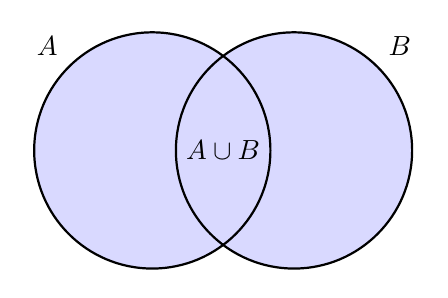
\begin{tikzpicture}[thick,
    set/.style = {circle,
        minimum size = 3cm,
        fill=blue!15}]

% Set A
\node[set,label={135:$A$}] (A) at (0,0) {};

% Set B
\node[set,label={45:$B$}] (B) at (1.8,0) {};

% Intersection
\begin{scope}
    \clip (0,0) circle(1.5cm);
    \clip (1.8,0) circle(1.5cm);
    \fill[blue!15](0,0) circle(1.5cm);
\end{scope}

% Circles outline
\draw (0,0) circle(1.5cm);
\draw (1.8,0) circle(1.5cm);

% Set intersection label
\node at (0.9,0) {$A\cup B$};

\end{tikzpicture}%
\hfill%
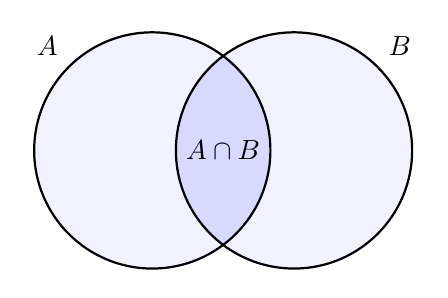
\begin{tikzpicture}[thick,
    set/.style = {circle,
        minimum size = 3cm,
        fill = blue!5}]

% Set A
\node[set,label={135:$A$}] (A) at (0,0) {};

% Set B
\node[set,label={45:$B$}] (B) at (1.8,0) {};

% Intersection
\begin{scope}
    \clip (0,0) circle(1.5cm);
    \clip (1.8,0) circle(1.5cm);
    \fill[blue!15](0,0) circle(1.5cm);
\end{scope}
% Circles outline
\draw (0,0) circle(1.5cm);
\draw (1.8,0) circle(1.5cm);

% Set intersection label
\node at (0.9,0) {$A\cap B$};

\end{tikzpicture}%
\hfill%
\vspace{2ex}

\hfill%
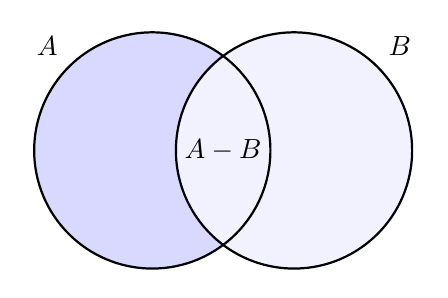
\begin{tikzpicture}[thick,
    set/.style = {circle,
        minimum size = 3cm}]

% Set A
\node[set,label={135:$A$},fill=blue!15] (A) at (0,0) {};

% Set B
\node[set,label={45:$B$},fill=blue!5] (B) at (1.8,0) {};

% Circles outline
\draw (0,0) circle(1.5cm);
\draw (1.8,0) circle(1.5cm);

% Set intersection label
\node at (0.9,0) {$A - B$};

\end{tikzpicture}%
\hfill%
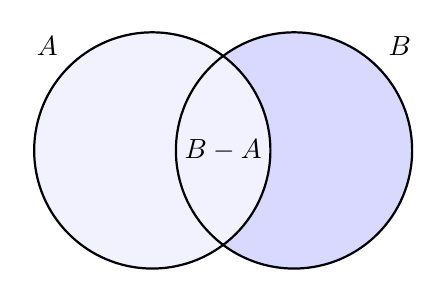
\begin{tikzpicture}[thick,
    set/.style = {circle,
        minimum size = 3cm}]

% Set B
\node[set,label={45:$B$},fill=blue!15] (B) at (1.8,0) {};

% Set A
\node[set,label={135:$A$},fill=blue!5] (A) at (0,0) {};

% Circles outline
\draw (0,0) circle(1.5cm);
\draw (1.8,0) circle(1.5cm);

% Set intersection label
\node at (0.9,0) {$B - A$};

\end{tikzpicture}%
\hfill%
\end{small}
\vspace{1ex}

In Bioinformatics it is usual, for example, to have character vectors of gene tags. We may have a vector for each of a set of different samples, and need to compare them. However, we start by using a more mundane example, everyday shopping, as illustration, followed by explanations.

\begin{knitrout}\footnotesize
\definecolor{shadecolor}{rgb}{0.969, 0.969, 0.969}\color{fgcolor}\begin{kframe}
\begin{alltt}
\hlstd{fruits} \hlkwb{<-} \hlkwd{c}\hlstd{(}\hlstr{"apple"}\hlstd{,} \hlstr{"pear"}\hlstd{,} \hlstr{"orange"}\hlstd{,} \hlstr{"lemon"}\hlstd{,} \hlstr{"tangerine"}\hlstd{)}
\hlstd{bakery} \hlkwb{<-} \hlkwd{c}\hlstd{(}\hlstr{"bread"}\hlstd{,} \hlstr{"buns"}\hlstd{,} \hlstr{"cake"}\hlstd{,} \hlstr{"cookies"}\hlstd{)}
\hlstd{dairy} \hlkwb{<-} \hlkwd{c}\hlstd{(}\hlstr{"milk"}\hlstd{,} \hlstr{"butter"}\hlstd{,} \hlstr{"cheese"}\hlstd{)}
\hlstd{shopping} \hlkwb{<-} \hlkwd{c}\hlstd{(}\hlstr{"bread"}\hlstd{,} \hlstr{"butter"}\hlstd{,} \hlstr{"apple"}\hlstd{,} \hlstr{"cheese"}\hlstd{,} \hlstr{"orange"}\hlstd{)}
\hlkwd{intersect}\hlstd{(fruits, shopping)}
\end{alltt}
\begin{verbatim}
## [1] "apple"  "orange"
\end{verbatim}
\begin{alltt}
\hlkwd{intersect}\hlstd{(bakery, shopping)}
\end{alltt}
\begin{verbatim}
## [1] "bread"
\end{verbatim}
\begin{alltt}
\hlkwd{intersect}\hlstd{(dairy, shopping)}
\end{alltt}
\begin{verbatim}
## [1] "butter" "cheese"
\end{verbatim}
\begin{alltt}
\hlstr{"lemon"} \hlopt \hlstd{dairy}
\end{alltt}
\begin{verbatim}
## [1] FALSE
\end{verbatim}
\begin{alltt}
\hlstr{"lemon"} \hlopt \hlstd{fruits}
\end{alltt}
\begin{verbatim}
## [1] TRUE
\end{verbatim}
\begin{alltt}
\hlstd{dairy} \hlopt \hlstd{shopping}
\end{alltt}
\begin{verbatim}
## [1] FALSE  TRUE  TRUE
\end{verbatim}
\begin{alltt}
\hlkwd{setdiff}\hlstd{(}\hlkwd{union}\hlstd{(bakery, dairy), shopping)}
\end{alltt}
\begin{verbatim}
## [1] "buns"    "cake"    "cookies" "milk"
\end{verbatim}
\end{kframe}
\end{knitrout}

For explanations we use abstract (symbolic) examples.

\begin{knitrout}\footnotesize
\definecolor{shadecolor}{rgb}{0.969, 0.969, 0.969}\color{fgcolor}\begin{kframe}
\begin{alltt}
\hlstd{my.set} \hlkwb{<-} \hlkwd{c}\hlstd{(}\hlstr{"a"}\hlstd{,} \hlstr{"b"}\hlstd{,} \hlstr{"c"}\hlstd{,} \hlstr{"b"}\hlstd{)}
\end{alltt}
\end{kframe}
\end{knitrout}

To test if a given value belongs to a set, we use operator \Roperator{\%in\%} or its function equivalent \Rfunction{is.element()}. In the algebra of sets notation, this is written $a \in A$, where $A$ is a set and $a$ a member. The second statement shows that the \code{\%in\%} operator is vectorized on its left-hand-side (lhs) operand, returning a logical vector.

\begin{knitrout}\footnotesize
\definecolor{shadecolor}{rgb}{0.969, 0.969, 0.969}\color{fgcolor}\begin{kframe}
\begin{alltt}
\hlkwd{is.element}\hlstd{(}\hlstr{"a"}\hlstd{, my.set)}
\end{alltt}
\begin{verbatim}
## [1] TRUE
\end{verbatim}
\begin{alltt}
\hlstr{"a"} \hlopt \hlstd{my.set}
\end{alltt}
\begin{verbatim}
## [1] TRUE
\end{verbatim}
\begin{alltt}
\hlkwd{c}\hlstd{(}\hlstr{"a"}\hlstd{,} \hlstr{"a"}\hlstd{,} \hlstr{"z"}\hlstd{)} \hlopt \hlstd{my.set}
\end{alltt}
\begin{verbatim}
## [1]  TRUE  TRUE FALSE
\end{verbatim}
\end{kframe}
\end{knitrout}

\begin{explainbox}
Keep in mind that inclusion is an asymmetrical (not reflective) operation among sets. The rhs argument is interpreted as a set, while the lhs argument is interpreted as a vector of values to test for inclusion. In other words, any duplicate member in the lhs will be retained while the rhs is interpreted as a set of unique values. The returned logical vector has the same length as the lhs.
\begin{knitrout}\footnotesize
\definecolor{shadecolor}{rgb}{0.969, 0.969, 0.969}\color{fgcolor}\begin{kframe}
\begin{alltt}
\hlstd{my.set} \hlopt \hlstr{"a"}
\end{alltt}
\begin{verbatim}
## [1]  TRUE FALSE FALSE FALSE
\end{verbatim}
\end{kframe}
\end{knitrout}
\end{explainbox}

The negation of inclusion is $a \not\in A$, and coded in \Rlang by applying the negation operator \Roperator{!} to the result of the test done with \Roperator{\%in\%} or function \Rfunction{is.element()}.

\begin{knitrout}\footnotesize
\definecolor{shadecolor}{rgb}{0.969, 0.969, 0.969}\color{fgcolor}\begin{kframe}
\begin{alltt}
\hlopt{!}\hlkwd{is.element}\hlstd{(}\hlstr{"a"}\hlstd{, my.set)}
\end{alltt}
\begin{verbatim}
## [1] FALSE
\end{verbatim}
\begin{alltt}
\hlopt{!}\hlstr{"a"} \hlopt \hlstd{my.set}
\end{alltt}
\begin{verbatim}
## [1] FALSE
\end{verbatim}
\begin{alltt}
\hlopt{!}\hlkwd{c}\hlstd{(}\hlstr{"a"}\hlstd{,} \hlstr{"a"}\hlstd{,} \hlstr{"z"}\hlstd{)} \hlopt \hlstd{my.set}
\end{alltt}
\begin{verbatim}
## [1] FALSE FALSE  TRUE
\end{verbatim}
\end{kframe}
\end{knitrout}

Although inclusion is a set operation, it is also very useful for the simplification of \code{if()\ldots else} statements by replacing multiple tests for alternative constant values of the same \code{mode} chained by multiple \Roperator{|} operators. A useful property of \Roperator{\%in\%} and \Rfunction{is.element()} is that they never return \code{NA}.

\begin{playground}
Use operator \Roperator{\%in\%} to write more concisely the following comparisons. Hint: see section \ref{sec:calc:boolean} on page \pageref{sec:calc:boolean} for the difference between \code{|} and \code{||} operators.

\begin{knitrout}\footnotesize
\definecolor{shadecolor}{rgb}{0.969, 0.969, 0.969}\color{fgcolor}\begin{kframe}
\begin{alltt}
\hlstd{x} \hlkwb{<-} \hlkwd{c}\hlstd{(}\hlstr{"a"}\hlstd{,} \hlstr{"a"}\hlstd{,} \hlstr{"z"}\hlstd{)}
\hlstd{x} \hlopt{==} \hlstr{"a"} \hlopt{|} \hlstd{x} \hlopt{==} \hlstr{"b"} \hlopt{|} \hlstd{x} \hlopt{==} \hlstr{"c"} \hlopt{|} \hlstd{x} \hlopt{==} \hlstr{"d"}
\end{alltt}
\end{kframe}
\end{knitrout}

Convert the \code{logical} vectors of length 3 into a vector of length one. Hint: see help for functions \code{all()} and \code{any()}.
\end{playground}

With \Rfunction{unique()} we convert a vector of possibly repeated values into a set of unique values. In the algebra of sets, a certain object belongs or not to a set. Consequently, in a set, multiple copies of the same object or value are meaningless.

\begin{knitrout}\footnotesize
\definecolor{shadecolor}{rgb}{0.969, 0.969, 0.969}\color{fgcolor}\begin{kframe}
\begin{alltt}
\hlkwd{unique}\hlstd{(my.set)}
\end{alltt}
\begin{verbatim}
## [1] "a" "b" "c"
\end{verbatim}
\begin{alltt}
\hlkwd{c}\hlstd{(}\hlstr{"a"}\hlstd{,} \hlstr{"a"}\hlstd{,} \hlstr{"z"}\hlstd{)} \hlopt \hlkwd{unique}\hlstd{(my.set)}
\end{alltt}
\begin{verbatim}
## [1]  TRUE  TRUE FALSE
\end{verbatim}
\end{kframe}
\end{knitrout}

In the notation used in algebra of sets, the set union operator is $\cup$ while the intersection operator is $\cap$. If we have sets $A$ and $B$, their union is given by $A \cup B$---in the next three examples, \code{c("a", "a", "z")} is a constant, while \code{my.set} is a variable.

\begin{knitrout}\footnotesize
\definecolor{shadecolor}{rgb}{0.969, 0.969, 0.969}\color{fgcolor}\begin{kframe}
\begin{alltt}
\hlkwd{union}\hlstd{(}\hlkwd{c}\hlstd{(}\hlstr{"a"}\hlstd{,} \hlstr{"a"}\hlstd{,} \hlstr{"z"}\hlstd{), my.set)}
\end{alltt}
\begin{verbatim}
## [1] "a" "z" "b" "c"
\end{verbatim}
\end{kframe}
\end{knitrout}

If we have sets $A$ and $B$, their intersection is given by $A \cap B$.

\begin{knitrout}\footnotesize
\definecolor{shadecolor}{rgb}{0.969, 0.969, 0.969}\color{fgcolor}\begin{kframe}
\begin{alltt}
\hlkwd{intersect}\hlstd{(}\hlkwd{c}\hlstd{(}\hlstr{"a"}\hlstd{,} \hlstr{"a"}\hlstd{,} \hlstr{"z"}\hlstd{), my.set)}
\end{alltt}
\begin{verbatim}
## [1] "a"
\end{verbatim}
\end{kframe}
\end{knitrout}

\begin{playground}
What do you expect to be the difference between the values returned by the three statements in the code chunk below? Before running them, write down your expectations about the value each one will return. Only then run the code. Independently of whether your predictions were correct or not, write down an explanation of what each statement's operation is.

\begin{knitrout}\footnotesize
\definecolor{shadecolor}{rgb}{0.969, 0.969, 0.969}\color{fgcolor}\begin{kframe}
\begin{alltt}
\hlkwd{union}\hlstd{(}\hlkwd{c}\hlstd{(}\hlstr{"a"}\hlstd{,} \hlstr{"a"}\hlstd{,} \hlstr{"z"}\hlstd{), my.set)}
\hlkwd{c}\hlstd{(}\hlkwd{c}\hlstd{(}\hlstr{"a"}\hlstd{,} \hlstr{"a"}\hlstd{,} \hlstr{"z"}\hlstd{), my.set)}
\hlkwd{c}\hlstd{(}\hlstr{"a"}\hlstd{,} \hlstr{"a"}\hlstd{,} \hlstr{"z"}\hlstd{, my.set)}
\end{alltt}
\end{kframe}
\end{knitrout}

In the algebra of sets notation $A \subseteq B$, where $A$ and $B$ are sets, indicates that $A$ is a subset or equal to $B$. For a true subset, the notation is $A \subset B$. The operators with the reverse direction are $\supseteq$ and $\supset$. Implement these four operations in four \Rlang statements, and test them on sets (represented by \Rlang vectors) with different ``overlap'' among set members.

\end{playground}

\begin{explainbox}
All set algebra examples above use character vectors and character constants. This is just the most frequent use case. Sets operations are valid on vectors of any atomic class, including \code{integer}, and computed values can be part of statements. In the second and third statements in the next chunk, we need to use additional parentheses to alter the default order of precedence between arithmetic and set operators.

\begin{knitrout}\footnotesize
\definecolor{shadecolor}{rgb}{0.969, 0.969, 0.969}\color{fgcolor}\begin{kframe}
\begin{alltt}
\hlnum{9L} \hlopt \hlnum{2L}\hlopt{:}\hlnum{4L}
\end{alltt}
\begin{verbatim}
## [1] FALSE
\end{verbatim}
\begin{alltt}
\hlnum{9L} \hlopt \hlstd{((}\hlnum{2L}\hlopt{:}\hlnum{4L}\hlstd{)} \hlopt{*} \hlstd{(}\hlnum{2L}\hlopt{:}\hlnum{4L}\hlstd{))}
\end{alltt}
\begin{verbatim}
## [1] TRUE
\end{verbatim}
\begin{alltt}
\hlkwd{c}\hlstd{(}\hlnum{1L}\hlstd{,} \hlnum{16L}\hlstd{)} \hlopt \hlstd{((}\hlnum{2L}\hlopt{:}\hlnum{4L}\hlstd{)} \hlopt{*} \hlstd{(}\hlnum{2L}\hlopt{:}\hlnum{4L}\hlstd{))}
\end{alltt}
\begin{verbatim}
## [1] FALSE  TRUE
\end{verbatim}
\end{kframe}
\end{knitrout}

\emph{Empty sets} are an important component of the algebra of sets, in \Rlang they are represented as vectors of zero length. Vectors and lists of zero length, which the \Rlang language fully supports, can be used to ``encode'' emptiness also in other contexts. These vectors do belong to a class such as \Rclass{numeric} or \Rclass{character} and must be compatible with other operands in an expression. By default, constructors for vectors, construct empty vectors.

\begin{knitrout}\footnotesize
\definecolor{shadecolor}{rgb}{0.969, 0.969, 0.969}\color{fgcolor}\begin{kframe}
\begin{alltt}
\hlkwd{length}\hlstd{(}\hlkwd{integer}\hlstd{())}
\end{alltt}
\begin{verbatim}
## [1] 0
\end{verbatim}
\end{kframe}
\end{knitrout}

\begin{knitrout}\footnotesize
\definecolor{shadecolor}{rgb}{0.969, 0.969, 0.969}\color{fgcolor}\begin{kframe}
\begin{alltt}
\hlnum{1L} \hlopt \hlkwd{integer}\hlstd{()}
\end{alltt}
\begin{verbatim}
## [1] FALSE
\end{verbatim}
\begin{alltt}
\hlkwd{setdiff}\hlstd{(}\hlnum{1L}\hlopt{:}\hlnum{4L}\hlstd{,} \hlkwd{union}\hlstd{(}\hlnum{1L}\hlopt{:}\hlnum{4L}\hlstd{,} \hlkwd{integer}\hlstd{()))}
\end{alltt}
\begin{verbatim}
## integer(0)
\end{verbatim}
\end{kframe}
\end{knitrout}

Although set operators are defined for \Rclass{numeric} vectors, rounding errors in `floats' can result in unexpected results (see section \ref{box:floats} on page \pageref{box:floats}). The next two examples do, however, return the correct answers.\qRoperator{\%in\%}

\begin{knitrout}\footnotesize
\definecolor{shadecolor}{rgb}{0.969, 0.969, 0.969}\color{fgcolor}\begin{kframe}
\begin{alltt}
\hlnum{9} \hlopt \hlstd{(}\hlnum{2}\hlopt{:}\hlnum{4}\hlstd{)}\hlopt{^}\hlnum{2}
\end{alltt}
\begin{verbatim}
## [1] TRUE
\end{verbatim}
\begin{alltt}
\hlkwd{c}\hlstd{(}\hlnum{1}\hlstd{,} \hlnum{5}\hlstd{)} \hlopt \hlstd{(}\hlnum{1}\hlopt{:}\hlnum{10}\hlstd{)}\hlopt{^}\hlnum{2}
\end{alltt}
\begin{verbatim}
## [1]  TRUE FALSE
\end{verbatim}
\end{kframe}
\end{knitrout}

\end{explainbox}
\index{operators!set|)}
\index{sets|)}

\section{Character values}\label{sec:calc:character}
\index{character strings}\index{classes and modes!character|(}\qRclass{character}
Character variables can be used to store any character. Character constants are written by enclosing characters in quotes. There are three types of quotes in the ASCII character set, double quotes \code{"}, single quotes \code{'}, and back ticks \code{`}. The first two types of quotes can be used as delimiters of \code{character} constants.

\begin{knitrout}\footnotesize
\definecolor{shadecolor}{rgb}{0.969, 0.969, 0.969}\color{fgcolor}\begin{kframe}
\begin{alltt}
\hlstd{a} \hlkwb{<-} \hlstr{"A"}
\hlstd{a}
\end{alltt}
\begin{verbatim}
## [1] "A"
\end{verbatim}
\begin{alltt}
\hlstd{b} \hlkwb{<-} \hlstr{'A'}
\hlstd{b}
\end{alltt}
\begin{verbatim}
## [1] "A"
\end{verbatim}
\begin{alltt}
\hlstd{a} \hlopt{==} \hlstd{b}
\end{alltt}
\begin{verbatim}
## [1] TRUE
\end{verbatim}
\end{kframe}
\end{knitrout}

\begin{explainbox}
In many computer languages, vectors of characters are distinct from vectors of character strings. In these languages, character vectors store at each index position a single character, while vectors of character strings store at each index position strings of characters of various lengths, such as words or sentences. If you are familiar with \Clang or \Cpplang, you need to keep in mind that \Clang's \code{char} and \Rlang's \code{character} are not equivalent and that in \Rlang, \code{character} vectors are vectors of character strings. In contrast to these other languages, in \Rlang there is no predefined class for vectors of individual characters and character constants enclosed in double or single quotes are not different.
\end{explainbox}

Concatenating character vectors of length one does not yield a longer character string, it yields instead a longer vector.
\begin{knitrout}\footnotesize
\definecolor{shadecolor}{rgb}{0.969, 0.969, 0.969}\color{fgcolor}\begin{kframe}
\begin{alltt}
\hlstd{a} \hlkwb{<-} \hlstr{'A'}
\hlstd{b} \hlkwb{<-} \hlstr{"bcdefg"}
\hlstd{c} \hlkwb{<-} \hlstr{"123"}
\hlstd{d} \hlkwb{<-} \hlkwd{c}\hlstd{(a, b, c)}
\hlstd{d}
\end{alltt}
\begin{verbatim}
## [1] "A"      "bcdefg" "123"
\end{verbatim}
\end{kframe}
\end{knitrout}

Having two different delimiters available makes it possible to choose the type of quotes used as delimiters so that other quotes can be included in a string.

\begin{knitrout}\footnotesize
\definecolor{shadecolor}{rgb}{0.969, 0.969, 0.969}\color{fgcolor}\begin{kframe}
\begin{alltt}
\hlstd{a} \hlkwb{<-} \hlstr{"He said 'hello' when he came in"}
\hlstd{a}
\end{alltt}
\begin{verbatim}
## [1] "He said 'hello' when he came in"
\end{verbatim}
\begin{alltt}
\hlstd{b} \hlkwb{<-} \hlstr{'He said "hello" when he came in'}
\hlstd{b}
\end{alltt}
\begin{verbatim}
## [1] "He said \"hello\" when he came in"
\end{verbatim}
\end{kframe}
\end{knitrout}

The\index{character string delimiters} outer quotes are not part of the string, they are ``delimiters'' used to mark the boundaries. As you can see when \code{b} is printed special characters can be represented using ``escape sequences''. There are several of them, and here we will show just four, new line (\verb|\n|) and tab (\verb|\t|), \verb|\"| the escape code for a quotation mark within a string and \verb|\\| the escape code for a single backslash \verb|\|. We also show here the different behavior of \Rfunction{print()} and \Rfunction{cat()}, with \Rfunction{cat()} \emph{interpreting} the escape sequences and \Rfunction{print()} displaying them as entered.

\begin{knitrout}\footnotesize
\definecolor{shadecolor}{rgb}{0.969, 0.969, 0.969}\color{fgcolor}\begin{kframe}
\begin{alltt}
\hlstd{c} \hlkwb{<-} \hlstr{"abc\textbackslash{}ndef\textbackslash{}tx\textbackslash{}"yz\textbackslash{}"\textbackslash{}\textbackslash{}\textbackslash{}tm"}
\hlkwd{print}\hlstd{(c)}
\end{alltt}
\begin{verbatim}
## [1] "abc\ndef\tx\"yz\"\\\tm"
\end{verbatim}
\begin{alltt}
\hlkwd{cat}\hlstd{(c)}
\end{alltt}
\begin{verbatim}
## abc
## def	x"yz"\	m
\end{verbatim}
\end{kframe}
\end{knitrout}

The \textit{escape codes}\index{character escape codes} work only in some contexts, as when using \Rfunction{cat()} to generate the output. For example, the new-line escape (\verb|\n|) can be embedded in strings used for axis-label, title or label in a plot to split them over two or more lines.
\index{classes and modes!character|)}

\section{The `mode' and `class' of objects}\label{sec:rlang:mode}
\index{objects!mode}
Variables have a \emph{mode} that depends on what is stored in them. But different from other languages, assignment to a variable of a different mode is allowed and in most cases its mode changes together with its contents. However, there is a restriction that all elements in a vector, array or matrix, must be of the same mode. While this is not required for lists, which can be heterogenous. In practice this means that we can assign an object, such as a vector, with a different \code{mode} to a name already in use, but we cannot use indexing to assign an object of a different mode to individual members of a vector, matrix or array. Functions with names starting with \code{is.} are tests returning a logical value, \code{TRUE}, \code{FALSE} or \code{NA}. Function \Rfunction{mode()} returns the mode of an object, as a character string and \Rfunction{typeof()} returns R's internal type or storage mode.\qRfunction{is.character()}\qRfunction{is.numeric()}\qRfunction{is.logical()}

\begin{knitrout}\footnotesize
\definecolor{shadecolor}{rgb}{0.969, 0.969, 0.969}\color{fgcolor}\begin{kframe}
\begin{alltt}
\hlstd{my_var} \hlkwb{<-} \hlnum{1}\hlopt{:}\hlnum{5}
\hlkwd{mode}\hlstd{(my_var)} \hlcom{# no distinction of integer or double}
\end{alltt}
\begin{verbatim}
## [1] "numeric"
\end{verbatim}
\begin{alltt}
\hlkwd{typeof}\hlstd{(my_var)}
\end{alltt}
\begin{verbatim}
## [1] "integer"
\end{verbatim}
\begin{alltt}
\hlkwd{is.numeric}\hlstd{(my_var)} \hlcom{# no distinction of integer or double}
\end{alltt}
\begin{verbatim}
## [1] TRUE
\end{verbatim}
\begin{alltt}
\hlkwd{is.double}\hlstd{(my_var)}
\end{alltt}
\begin{verbatim}
## [1] FALSE
\end{verbatim}
\begin{alltt}
\hlkwd{is.integer}\hlstd{(my_var)}
\end{alltt}
\begin{verbatim}
## [1] TRUE
\end{verbatim}
\begin{alltt}
\hlkwd{is.logical}\hlstd{(my_var)}
\end{alltt}
\begin{verbatim}
## [1] FALSE
\end{verbatim}
\begin{alltt}
\hlkwd{is.character}\hlstd{(my_var)}
\end{alltt}
\begin{verbatim}
## [1] FALSE
\end{verbatim}
\begin{alltt}
\hlstd{my_var} \hlkwb{<-} \hlstr{"abc"}
\hlkwd{mode}\hlstd{(my_var)}
\end{alltt}
\begin{verbatim}
## [1] "character"
\end{verbatim}
\end{kframe}
\end{knitrout}

While \emph{mode} is a fundamental property, and limited to those modes defined as part of the \Rlang language, the concept of \emph{class}, is different in that new classes can be defined in user code. In particular, different \Rlang objects of a given mode, such as \code{numeric}, can belong to different \code{class}es. The use of classes for dispatching functions is discussed in section \ref{sec:script:objects:classes:methods} on page \pageref{sec:script:objects:classes:methods}, in relation to object-oriented programming in \Rlang. Method \Rfunction{class()} is used to query the class of an object, and method \Rfunction{inherits()} is used to test if an object belongs to a specific class or not (including ``parent'' classes, to be later described).

\begin{knitrout}\footnotesize
\definecolor{shadecolor}{rgb}{0.969, 0.969, 0.969}\color{fgcolor}\begin{kframe}
\begin{alltt}
\hlkwd{class}\hlstd{(my_var)}
\end{alltt}
\begin{verbatim}
## [1] "character"
\end{verbatim}
\begin{alltt}
\hlkwd{inherits}\hlstd{(my_var,} \hlstr{"character"}\hlstd{)}
\end{alltt}
\begin{verbatim}
## [1] TRUE
\end{verbatim}
\begin{alltt}
\hlkwd{inherits}\hlstd{(my_var,} \hlstr{"numeric"}\hlstd{)}
\end{alltt}
\begin{verbatim}
## [1] FALSE
\end{verbatim}
\end{kframe}
\end{knitrout}

\section{`Type' conversions}\label{sec:calc:type:conversion}
\index{type conversion|(}
The least-intuitive type conversions are those related to logical values. All others are as one would expect. By convention, functions used to convert objects from one mode to a different one have names starting with \code{as.}\footnote{Except for some packages in the \pkgnameNI{tidyverse} that use names starting with \code{as\_} instead of \code{as.}.}.\qRfunction{as.character()}\qRfunction{as.numeric()}\qRfunction{as.logical()}

\begin{knitrout}\footnotesize
\definecolor{shadecolor}{rgb}{0.969, 0.969, 0.969}\color{fgcolor}\begin{kframe}
\begin{alltt}
\hlkwd{as.character}\hlstd{(}\hlnum{1}\hlstd{)}
\end{alltt}
\begin{verbatim}
## [1] "1"
\end{verbatim}
\begin{alltt}
\hlkwd{as.numeric}\hlstd{(}\hlstr{"1"}\hlstd{)}
\end{alltt}
\begin{verbatim}
## [1] 1
\end{verbatim}
\begin{alltt}
\hlkwd{as.logical}\hlstd{(}\hlstr{"TRUE"}\hlstd{)}
\end{alltt}
\begin{verbatim}
## [1] TRUE
\end{verbatim}
\begin{alltt}
\hlkwd{as.logical}\hlstd{(}\hlstr{"NA"}\hlstd{)}
\end{alltt}
\begin{verbatim}
## [1] NA
\end{verbatim}
\end{kframe}
\end{knitrout}

Conversion takes place automatically in arithmetic and logical expressions.

\begin{knitrout}\footnotesize
\definecolor{shadecolor}{rgb}{0.969, 0.969, 0.969}\color{fgcolor}\begin{kframe}
\begin{alltt}
\hlnum{TRUE} \hlopt{+} \hlnum{10}
\end{alltt}
\begin{verbatim}
## [1] 11
\end{verbatim}
\begin{alltt}
\hlnum{1} \hlopt{||} \hlnum{0}
\end{alltt}
\begin{verbatim}
## [1] TRUE
\end{verbatim}
\begin{alltt}
\hlnum{FALSE} \hlopt{| -}\hlnum{2}\hlopt{:}\hlnum{2}
\end{alltt}
\begin{verbatim}
## [1]  TRUE  TRUE FALSE  TRUE  TRUE
\end{verbatim}
\end{kframe}
\end{knitrout}

\begin{playground}
There is some flexibility in the conversion from character strings into \code{numeric} and \code{logical} values. Use the examples below plus your own variations to get an idea of what strings are acceptable and correctly converted and which are not. Do also pay attention at the conversion between \code{numeric} and \code{logical} values.\qRfunction{as.character()}\qRfunction{as.numeric()}\qRfunction{as.logical()}

\begin{knitrout}\footnotesize
\definecolor{shadecolor}{rgb}{0.969, 0.969, 0.969}\color{fgcolor}\begin{kframe}
\begin{alltt}
\hlkwd{as.character}\hlstd{(}\hlnum{3.0e10}\hlstd{)}
\hlkwd{as.numeric}\hlstd{(}\hlstr{"5E+5"}\hlstd{)}
\hlkwd{as.numeric}\hlstd{(}\hlstr{"A"}\hlstd{)}
\hlkwd{as.numeric}\hlstd{(}\hlnum{TRUE}\hlstd{)}
\hlkwd{as.numeric}\hlstd{(}\hlnum{FALSE}\hlstd{)}
\hlkwd{as.logical}\hlstd{(}\hlstr{"T"}\hlstd{)}
\hlkwd{as.logical}\hlstd{(}\hlstr{"t"}\hlstd{)}
\hlkwd{as.logical}\hlstd{(}\hlstr{"true"}\hlstd{)}
\hlkwd{as.logical}\hlstd{(}\hlnum{100}\hlstd{)}
\hlkwd{as.logical}\hlstd{(}\hlnum{0}\hlstd{)}
\hlkwd{as.logical}\hlstd{(}\hlopt{-}\hlnum{1}\hlstd{)}
\end{alltt}
\end{kframe}
\end{knitrout}

\end{playground}

\begin{playground}
Compare the values returned by \Rfunction{trunc()} and \Rfunction{as.integer()} when applied to a floating point number, such as \code{12.34}. Check for the equality of values, and for the \emph{class} of the returned objects.
\end{playground}

\begin{explainbox}
Using conversions, the difference between the length of a \code{character} vector and the number of characters composing each member ``string'' within a vector is obvious.\qRfunction{length()}\qRfunction{as.numeric()}

\begin{knitrout}\footnotesize
\definecolor{shadecolor}{rgb}{0.969, 0.969, 0.969}\color{fgcolor}\begin{kframe}
\begin{alltt}
\hlstd{f} \hlkwb{<-} \hlkwd{c}\hlstd{(}\hlstr{"1"}\hlstd{,} \hlstr{"2"}\hlstd{,} \hlstr{"3"}\hlstd{)}
\hlkwd{length}\hlstd{(f)}
\end{alltt}
\begin{verbatim}
## [1] 3
\end{verbatim}
\begin{alltt}
\hlstd{g} \hlkwb{<-} \hlstr{"123"}
\hlkwd{length}\hlstd{(g)}
\end{alltt}
\begin{verbatim}
## [1] 1
\end{verbatim}
\begin{alltt}
\hlkwd{as.numeric}\hlstd{(f)}
\end{alltt}
\begin{verbatim}
## [1] 1 2 3
\end{verbatim}
\begin{alltt}
\hlkwd{as.numeric}\hlstd{(g)}
\end{alltt}
\begin{verbatim}
## [1] 123
\end{verbatim}
\end{kframe}
\end{knitrout}
\end{explainbox}

\sloppy
Other\index{formatted character strings from numbers} functions relevant to the ``conversion'' of numbers and other values are \Rfunction{format()}, and \Rfunction{sprintf()}. These two functions return \Rclass{character} strings, instead of \code{numeric} or other values, and are useful for printing output. One could think of these functions as advanced conversion functions returning formatted, and possibly combined and annotated, character strings. However, they are usually not considered normal conversion functions, as they are very rarely used in a way that preserves the original precision of the input values. We show here the use of \Rfunction{format()} and \Rfunction{sprintf()} with \code{numeric} values, but they can also be used with values of other modes.

When using \Rfunction{format()}, the format used to display numbers is set by passing arguments to several different parameters. As \Rfunction{print()} calls \Rfunction{format()} to make numbers \emph{pretty} it accepts the same options.

\begin{knitrout}\footnotesize
\definecolor{shadecolor}{rgb}{0.969, 0.969, 0.969}\color{fgcolor}\begin{kframe}
\begin{alltt}
\hlstd{x} \hlkwb{=} \hlkwd{c}\hlstd{(}\hlnum{123.4567890}\hlstd{,} \hlnum{1.0}\hlstd{)}
\hlkwd{format}\hlstd{(x)} \hlcom{# using defaults}
\end{alltt}
\begin{verbatim}
## [1] "123.4568" "  1.0000"
\end{verbatim}
\begin{alltt}
\hlkwd{format}\hlstd{(x[}\hlnum{1}\hlstd{])} \hlcom{# using defaults}
\end{alltt}
\begin{verbatim}
## [1] "123.4568"
\end{verbatim}
\begin{alltt}
\hlkwd{format}\hlstd{(x[}\hlnum{2}\hlstd{])} \hlcom{# using defaults}
\end{alltt}
\begin{verbatim}
## [1] "1"
\end{verbatim}
\begin{alltt}
\hlkwd{format}\hlstd{(x,} \hlkwc{digits} \hlstd{=} \hlnum{3}\hlstd{,} \hlkwc{nsmall} \hlstd{=} \hlnum{1}\hlstd{)}
\end{alltt}
\begin{verbatim}
## [1] "123.5" "  1.0"
\end{verbatim}
\begin{alltt}
\hlkwd{format}\hlstd{(x[}\hlnum{1}\hlstd{],} \hlkwc{digits} \hlstd{=} \hlnum{3}\hlstd{,} \hlkwc{nsmall} \hlstd{=} \hlnum{1}\hlstd{)}
\end{alltt}
\begin{verbatim}
## [1] "123.5"
\end{verbatim}
\begin{alltt}
\hlkwd{format}\hlstd{(x[}\hlnum{2}\hlstd{],} \hlkwc{digits} \hlstd{=} \hlnum{3}\hlstd{,} \hlkwc{nsmall} \hlstd{=} \hlnum{1}\hlstd{)}
\end{alltt}
\begin{verbatim}
## [1] "1.0"
\end{verbatim}
\begin{alltt}
\hlkwd{format}\hlstd{(x,} \hlkwc{digits} \hlstd{=} \hlnum{3}\hlstd{,} \hlkwc{scientific} \hlstd{=} \hlnum{TRUE}\hlstd{)}
\end{alltt}
\begin{verbatim}
## [1] "1.23e+02" "1.00e+00"
\end{verbatim}
\end{kframe}
\end{knitrout}

Function \Rfunction{sprintf()} is similar to \Clang's function of the same name. The user interface is rather unusual, but very powerful, once one learns the syntax. All the formatting is specified using a \code{character} string as template. In this template, placeholders for data and the formatting instructions are embedded using special codes. These codes start with a percent character. We show in the example below the use of some of these: \code{f} is used for \code{numeric} values to be formatted according to a ``fixed point,'' while \code{g} is used when we set the number of significant digits and \code{e} for exponential or \emph{scientific} notation.

\begin{knitrout}\footnotesize
\definecolor{shadecolor}{rgb}{0.969, 0.969, 0.969}\color{fgcolor}\begin{kframe}
\begin{alltt}
\hlstd{x} \hlkwb{=} \hlkwd{c}\hlstd{(}\hlnum{123.4567890}\hlstd{,} \hlnum{1.0}\hlstd{)}
\hlkwd{sprintf}\hlstd{(}\hlstr{"The numbers are: %4.2f and %.0f"}\hlstd{, x[}\hlnum{1}\hlstd{], x[}\hlnum{2}\hlstd{])}
\end{alltt}
\begin{verbatim}
## [1] "The numbers are: 123.46 and 1"
\end{verbatim}
\begin{alltt}
\hlkwd{sprintf}\hlstd{(}\hlstr{"The numbers are: %.4g and %.2g"}\hlstd{, x[}\hlnum{1}\hlstd{], x[}\hlnum{2}\hlstd{])}
\end{alltt}
\begin{verbatim}
## [1] "The numbers are: 123.5 and 1"
\end{verbatim}
\begin{alltt}
\hlkwd{sprintf}\hlstd{(}\hlstr{"The numbers are: %4.2e and %.0e"}\hlstd{, x[}\hlnum{1}\hlstd{], x[}\hlnum{2}\hlstd{])}
\end{alltt}
\begin{verbatim}
## [1] "The numbers are: 1.23e+02 and 1e+00"
\end{verbatim}
\end{kframe}
\end{knitrout}

In the template \code{"The numbers are: \%4.2f and \%.0f"}, there are two placeholders for \code{numeric} values, \code{\%4.2f} and \code{\%.0f}, so in addition to the template, we pass two values extracted from the first two positions of vector \code{x}. These could have been two different vectors of length one, or even numeric constants. The template itself does not need to be a \code{character} constant as in these examples, as a variable can be also passed as argument.

\begin{playground}
Function \Rfunction{format()} may be easier to use, in some cases, but \Rfunction{sprintf()} is more flexible and powerful. Those with experience in the use of the \Clang language will already know about \Rfunction{sprintf()} and its use of templates for formatting output. Even if you are familiar with  \Clang, look up the help pages for both functions, and practice, by trying to create the same formatted output by means of the two functions. Do also play with these functions with other types of data like \code{integer} and \code{character}.
\end{playground}

\begin{explainbox}
We have above described \Rconst{NA} as a single value ignoring modes, but in reality \Rconst{NA}s come in various flavors. \Rconst{NA\_real\_}, \Rconst{NA\_character\_}, etc. and \Rconst{NA} defaults to an \Rconst{NA} of class \Rclass{logical}. \Rconst{NA} is normally converted on the fly to other modes when needed, so in general \Rconst{NA} is all we need to use.

\begin{knitrout}\footnotesize
\definecolor{shadecolor}{rgb}{0.969, 0.969, 0.969}\color{fgcolor}\begin{kframe}
\begin{alltt}
\hlstd{a} \hlkwb{<-} \hlkwd{c}\hlstd{(}\hlnum{1}\hlstd{,} \hlnum{NA}\hlstd{)}
\hlkwd{is.numeric}\hlstd{(a[}\hlnum{2}\hlstd{])}
\end{alltt}
\begin{verbatim}
## [1] TRUE
\end{verbatim}
\begin{alltt}
\hlkwd{is.numeric}\hlstd{(}\hlnum{NA}\hlstd{)}
\end{alltt}
\begin{verbatim}
## [1] FALSE
\end{verbatim}
\end{kframe}
\end{knitrout}

\begin{knitrout}\footnotesize
\definecolor{shadecolor}{rgb}{0.969, 0.969, 0.969}\color{fgcolor}\begin{kframe}
\begin{alltt}
\hlstd{b} \hlkwb{<-} \hlkwd{c}\hlstd{(}\hlstr{"abc"}\hlstd{,} \hlnum{NA}\hlstd{)}
\hlkwd{is.character}\hlstd{(b[}\hlnum{2}\hlstd{])}
\end{alltt}
\begin{verbatim}
## [1] TRUE
\end{verbatim}
\end{kframe}
\end{knitrout}

\begin{knitrout}\footnotesize
\definecolor{shadecolor}{rgb}{0.969, 0.969, 0.969}\color{fgcolor}\begin{kframe}
\begin{alltt}
\hlkwd{is.character}\hlstd{(}\hlnum{NA}\hlstd{)}
\end{alltt}
\begin{verbatim}
## [1] FALSE
\end{verbatim}
\begin{alltt}
\hlkwd{class}\hlstd{(}\hlnum{NA}\hlstd{)}
\end{alltt}
\begin{verbatim}
## [1] "logical"
\end{verbatim}
\begin{alltt}
\hlkwd{class}\hlstd{(}\hlnum{NA_character_}\hlstd{)}
\end{alltt}
\begin{verbatim}
## [1] "character"
\end{verbatim}
\end{kframe}
\end{knitrout}

\begin{knitrout}\footnotesize
\definecolor{shadecolor}{rgb}{0.969, 0.969, 0.969}\color{fgcolor}\begin{kframe}
\begin{alltt}
\hlstd{c} \hlkwb{<-} \hlnum{NA}
\hlkwd{c}\hlstd{(c,} \hlnum{2}\hlopt{:}\hlnum{3}\hlstd{)}
\end{alltt}
\begin{verbatim}
## [1] NA  2  3
\end{verbatim}
\end{kframe}
\end{knitrout}

However, even the statement below works transparently.

\begin{knitrout}\footnotesize
\definecolor{shadecolor}{rgb}{0.969, 0.969, 0.969}\color{fgcolor}\begin{kframe}
\begin{alltt}
\hlstd{a[}\hlnum{3}\hlstd{]} \hlkwb{<-} \hlstd{b[}\hlnum{2}\hlstd{]}
\end{alltt}
\end{kframe}
\end{knitrout}
\end{explainbox}

\index{type conversion|)}

\section{Vector manipulation}\label{sec:vectors}\label{sec:calc:indexing}
\index{vectors!indexing|(}\index{vectors!member extraction}
If you have read earlier sections of this chapter, you already know how to create a vector. \Rlang's vectors are equivalent to what would be written in mathematical notation as $a_{1\ldots n} = a_1, a_2, \ldots, a_i, \ldots, a_n$, they are not the equivalent to the vectors, common in Physics, which are symbolized with an arrow as an ``accent,'' such as $\overrightarrow{\mathbf{F}}$.

In this section we are going to see how to extract or retrieve, replace, and move elements such as $a_2$ from a vector. Elements are extracted using an index enclosed in single square brackets. The index indicates the position in the vector, starting from one, following the usual mathematical tradition. We here use a vector of characters to make it clear the distinction between contents of the vector from the numerical indexes. What in maths notation would be $a_i$ for a vector $a_{1\ldots n}$, in \Rpgrm is represented as \code{a[i]} and the whole vector, by excluding the brackets and indexing vector, as \code{a}.

\begin{knitrout}\footnotesize
\definecolor{shadecolor}{rgb}{0.969, 0.969, 0.969}\color{fgcolor}\begin{kframe}
\begin{alltt}
\hlstd{a} \hlkwb{<-} \hlstd{letters[}\hlnum{1}\hlopt{:}\hlnum{10}\hlstd{]}
\hlstd{a}
\end{alltt}
\begin{verbatim}
##  [1] "a" "b" "c" "d" "e" "f" "g" "h" "i" "j"
\end{verbatim}
\begin{alltt}
\hlstd{a[}\hlnum{2}\hlstd{]}
\end{alltt}
\begin{verbatim}
## [1] "b"
\end{verbatim}
\end{kframe}
\end{knitrout}

\begin{explainbox}
Four constant vectors are available in \Rlang: \Rconst{letters}, \Rconst{LETTERS}, \Rconst{month.name} and  \Rconst{month.abb}, of which we used \code{letters} in the example above. These vectors are always for English, irrespective of the locale.
\end{explainbox}

\begin{warningbox}
In \Rlang, indexes always start from one, while in some other programming languages such as \Clang and \Cpplang, indexes start from zero. It is important to be aware of this difference, as many computation algorithms are valid only under a given indexing convention.
\end{warningbox}

It is possible to extract a subset of the elements of a vector in a single operation, using a vector of indexes. The positions of the extracted elements in the result (``returned value'') are determined by the ordering of the members of the vector of indexes---easier to demonstrate than to explain.

\begin{knitrout}\footnotesize
\definecolor{shadecolor}{rgb}{0.969, 0.969, 0.969}\color{fgcolor}\begin{kframe}
\begin{alltt}
\hlstd{a[}\hlkwd{c}\hlstd{(}\hlnum{3}\hlstd{,} \hlnum{2}\hlstd{)]}
\end{alltt}
\begin{verbatim}
## [1] "c" "b"
\end{verbatim}
\begin{alltt}
\hlstd{a[}\hlnum{10}\hlopt{:}\hlnum{1}\hlstd{]}
\end{alltt}
\begin{verbatim}
##  [1] "j" "i" "h" "g" "f" "e" "d" "c" "b" "a"
\end{verbatim}
\end{kframe}
\end{knitrout}

\begin{playground}
The length of the indexing vector is not restricted by the length of the indexed vector. However, only numerical indexes that match positions present in the indexed vector can extract values. Those values in the indexing vector pointing to positions that are not present in the indexed vector, result in \code{NA}s. This is easier to learn by \emph{playing} with \Rlang, than from explanations. Play with \Rlang, using the following examples as a starting point.

\begin{knitrout}\footnotesize
\definecolor{shadecolor}{rgb}{0.969, 0.969, 0.969}\color{fgcolor}\begin{kframe}
\begin{alltt}
\hlkwd{length}\hlstd{(a)}
\hlstd{a[}\hlkwd{c}\hlstd{(}\hlnum{3}\hlstd{,} \hlnum{3}\hlstd{,} \hlnum{3}\hlstd{,} \hlnum{3}\hlstd{)]}
\hlstd{a[}\hlkwd{c}\hlstd{(}\hlnum{10}\hlopt{:}\hlnum{1}\hlstd{,} \hlnum{1}\hlopt{:}\hlnum{10}\hlstd{)]}
\hlstd{a[}\hlkwd{c}\hlstd{(}\hlnum{1}\hlstd{,} \hlnum{11}\hlstd{)]}
\hlstd{a[}\hlnum{11}\hlstd{]}
\end{alltt}
\end{kframe}
\end{knitrout}

Have you tried some of your own examples? If not yet, do \emph{play} with additional variations of your own before continuing.

\end{playground}

Negative indexes have a special meaning; they indicate the positions at which values should be excluded. Be aware that it is \emph{illegal} to mix positive and negative values in the same indexing operation.

\begin{knitrout}\footnotesize
\definecolor{shadecolor}{rgb}{0.969, 0.969, 0.969}\color{fgcolor}\begin{kframe}
\begin{alltt}
\hlstd{a[}\hlopt{-}\hlnum{2}\hlstd{]}
\end{alltt}
\begin{verbatim}
## [1] "a" "c" "d" "e" "f" "g" "h" "i" "j"
\end{verbatim}
\begin{alltt}
\hlstd{a[}\hlopt{-}\hlkwd{c}\hlstd{(}\hlnum{3}\hlstd{,}\hlnum{2}\hlstd{)]}
\end{alltt}
\begin{verbatim}
## [1] "a" "d" "e" "f" "g" "h" "i" "j"
\end{verbatim}
\begin{alltt}
\hlstd{a[}\hlopt{-}\hlnum{3}\hlopt{:-}\hlnum{2}\hlstd{]}
\end{alltt}
\begin{verbatim}
## [1] "a" "d" "e" "f" "g" "h" "i" "j"
\end{verbatim}
\end{kframe}
\end{knitrout}

\begin{advplayground}
Results from indexing with special values and zero may be surprising. Try to build a rule from the examples below, a rule that will help you remember what to expect next time you are confronted with similar statements using ``subscripts'' which are special values instead of integers larger or equal to one---this is likely to happen sooner or later as these special values can be returned by different \Rlang expressions depending on the value of operands or function arguments, some of them described earlier in this chapter.

\begin{knitrout}\footnotesize
\definecolor{shadecolor}{rgb}{0.969, 0.969, 0.969}\color{fgcolor}\begin{kframe}
\begin{alltt}
\hlstd{a[ ]}
\hlstd{a[}\hlnum{0}\hlstd{]}
\hlstd{a[}\hlkwd{numeric}\hlstd{(}\hlnum{0}\hlstd{)]}
\hlstd{a[}\hlnum{NA}\hlstd{]}
\hlstd{a[}\hlkwd{c}\hlstd{(}\hlnum{1}\hlstd{,} \hlnum{NA}\hlstd{)]}
\hlstd{a[}\hlkwa{NULL}\hlstd{]}
\hlstd{a[}\hlkwd{c}\hlstd{(}\hlnum{1}\hlstd{,} \hlkwa{NULL}\hlstd{)]}
\end{alltt}
\end{kframe}
\end{knitrout}
\end{advplayground}

Another way of indexing, which is very handy, but not available in most other programming languages, is indexing with a vector of \code{logical} values. The \code{logical} vector used for indexing is usually of the same length as the vector from which elements are going to be selected. However, this is not a requirement, because if the \code{logical} vector of indexes is shorter than the indexed vector, it is ``recycled'' as discussed above in relation to other operators.

\begin{knitrout}\footnotesize
\definecolor{shadecolor}{rgb}{0.969, 0.969, 0.969}\color{fgcolor}\begin{kframe}
\begin{alltt}
\hlstd{a[}\hlnum{TRUE}\hlstd{]}
\end{alltt}
\begin{verbatim}
##  [1] "a" "b" "c" "d" "e" "f" "g" "h" "i" "j"
\end{verbatim}
\begin{alltt}
\hlstd{a[}\hlnum{FALSE}\hlstd{]}
\end{alltt}
\begin{verbatim}
## character(0)
\end{verbatim}
\begin{alltt}
\hlstd{a[}\hlkwd{c}\hlstd{(}\hlnum{TRUE}\hlstd{,} \hlnum{FALSE}\hlstd{)]}
\end{alltt}
\begin{verbatim}
## [1] "a" "c" "e" "g" "i"
\end{verbatim}
\begin{alltt}
\hlstd{a[}\hlkwd{c}\hlstd{(}\hlnum{FALSE}\hlstd{,} \hlnum{TRUE}\hlstd{)]}
\end{alltt}
\begin{verbatim}
## [1] "b" "d" "f" "h" "j"
\end{verbatim}
\begin{alltt}
\hlstd{a} \hlopt{>} \hlstr{"c"}
\end{alltt}
\begin{verbatim}
##  [1] FALSE FALSE FALSE  TRUE  TRUE  TRUE  TRUE  TRUE  TRUE  TRUE
\end{verbatim}
\begin{alltt}
\hlstd{a[a} \hlopt{>} \hlstr{"c"}\hlstd{]}
\end{alltt}
\begin{verbatim}
## [1] "d" "e" "f" "g" "h" "i" "j"
\end{verbatim}
\end{kframe}
\end{knitrout}

Indexing with logical vectors is very frequently used in \Rlang because comparison operators are vectorized. Comparison operators, when applied to a vector, return a \code{logical} vector, a vector that can be used to extract the elements for which the result of the comparison test was \code{TRUE}.

\begin{playground}
The examples in this text box demonstrate additional uses of logical vectors: 1) the logical vector returned by a vectorized comparison can be stored in a variable, and the variable used as a ``selector'' for extracting a subset of values from the same vector, or from a different vector.

\begin{knitrout}\footnotesize
\definecolor{shadecolor}{rgb}{0.969, 0.969, 0.969}\color{fgcolor}\begin{kframe}
\begin{alltt}
\hlstd{a} \hlkwb{<-} \hlstd{letters[}\hlnum{1}\hlopt{:}\hlnum{10}\hlstd{]}
\hlstd{b} \hlkwb{<-} \hlnum{1}\hlopt{:}\hlnum{10}
\hlstd{selector} \hlkwb{<-} \hlstd{a} \hlopt{>} \hlstr{"c"}
\hlstd{selector}
\hlstd{a[selector]}
\hlstd{b[selector]}
\end{alltt}
\end{kframe}
\end{knitrout}

Numerical indexes can be obtained from a logical vector by means of function \code{which()}.

\begin{knitrout}\footnotesize
\definecolor{shadecolor}{rgb}{0.969, 0.969, 0.969}\color{fgcolor}\begin{kframe}
\begin{alltt}
\hlstd{indexes} \hlkwb{<-} \hlkwd{which}\hlstd{(a} \hlopt{>} \hlstr{"c"}\hlstd{)}
\hlstd{indexes}
\hlstd{a[indexes]}
\hlstd{b[indexes]}
\end{alltt}
\end{kframe}
\end{knitrout}

Make sure to understand the examples above. These constructs are very widely used in \Rlang because they allow for concise code that is easy to understand once you are familiar with the indexing rules. However, if you do not command these rules, many of these terse statements will be unintelligible to you.
\end{playground}

Indexing can be used on either side of an assignment expression. In the chunk below, we use the extraction operator on the left-hand side of the assignments to replace values only at selected positions in the vector. This may look rather esoteric at first sight, but it is just a simple extension of the logic of indexing described above. It works, because the low precedence of the \Roperator{<-} operator results in both the left-hand side and the right-hand side being fully evaluated before the assignment takes place. To make the changes to the vectors easier to follow, we use identical vectors with different names for each of these examples.

\begin{knitrout}\footnotesize
\definecolor{shadecolor}{rgb}{0.969, 0.969, 0.969}\color{fgcolor}\begin{kframe}
\begin{alltt}
\hlstd{a} \hlkwb{<-} \hlnum{1}\hlopt{:}\hlnum{10}
\hlstd{a}
\end{alltt}
\begin{verbatim}
##  [1]  1  2  3  4  5  6  7  8  9 10
\end{verbatim}
\begin{alltt}
\hlstd{a[}\hlnum{1}\hlstd{]} \hlkwb{<-} \hlnum{99}
\hlstd{a}
\end{alltt}
\begin{verbatim}
##  [1] 99  2  3  4  5  6  7  8  9 10
\end{verbatim}
\begin{alltt}
\hlstd{b} \hlkwb{<-} \hlnum{1}\hlopt{:}\hlnum{10}
\hlstd{b[}\hlkwd{c}\hlstd{(}\hlnum{2}\hlstd{,}\hlnum{4}\hlstd{)]} \hlkwb{<-} \hlopt{-}\hlnum{99} \hlcom{# recycling}
\hlstd{b}
\end{alltt}
\begin{verbatim}
##  [1]   1 -99   3 -99   5   6   7   8   9  10
\end{verbatim}
\begin{alltt}
\hlstd{c} \hlkwb{<-} \hlnum{1}\hlopt{:}\hlnum{10}
\hlstd{c[}\hlkwd{c}\hlstd{(}\hlnum{2}\hlstd{,}\hlnum{4}\hlstd{)]} \hlkwb{<-} \hlkwd{c}\hlstd{(}\hlopt{-}\hlnum{99}\hlstd{,} \hlnum{99}\hlstd{)}
\hlstd{c}
\end{alltt}
\begin{verbatim}
##  [1]   1 -99   3  99   5   6   7   8   9  10
\end{verbatim}
\begin{alltt}
\hlstd{d} \hlkwb{<-} \hlnum{1}\hlopt{:}\hlnum{10}
\hlstd{d[}\hlnum{TRUE}\hlstd{]} \hlkwb{<-} \hlnum{1} \hlcom{# recycling}
\hlstd{d}
\end{alltt}
\begin{verbatim}
##  [1] 1 1 1 1 1 1 1 1 1 1
\end{verbatim}
\begin{alltt}
\hlstd{e} \hlkwb{<-} \hlnum{1}\hlopt{:}\hlnum{10}
\hlstd{e} \hlkwb{<-} \hlnum{1}  \hlcom{# no recycling}
\hlstd{e}
\end{alltt}
\begin{verbatim}
## [1] 1
\end{verbatim}
\end{kframe}
\end{knitrout}

We can also use subscripting on both sides of the assignment operator, for example, to swap two elements.

\begin{knitrout}\footnotesize
\definecolor{shadecolor}{rgb}{0.969, 0.969, 0.969}\color{fgcolor}\begin{kframe}
\begin{alltt}
\hlstd{a} \hlkwb{<-} \hlstd{letters[}\hlnum{1}\hlopt{:}\hlnum{10}\hlstd{]}
\hlstd{a[}\hlnum{1}\hlopt{:}\hlnum{2}\hlstd{]} \hlkwb{<-} \hlstd{a[}\hlnum{2}\hlopt{:}\hlnum{1}\hlstd{]}
\hlstd{a}
\end{alltt}
\begin{verbatim}
##  [1] "b" "a" "c" "d" "e" "f" "g" "h" "i" "j"
\end{verbatim}
\end{kframe}
\end{knitrout}

\begin{playground}
Do play with subscripts to your heart's content, really grasping how they work and how they can be used, will be very useful in anything you do in the future with \Rlang. Even the contrived example below follows the same simple rules, just study it bit by bit. Hint: the second statement in the chunk below, modifies \code{a}, so, when studying variations of this example you will need to recreate \code{a} by executing the first statement, each time you run a variation of the second statement.

\begin{knitrout}\footnotesize
\definecolor{shadecolor}{rgb}{0.969, 0.969, 0.969}\color{fgcolor}\begin{kframe}
\begin{alltt}
\hlstd{a} \hlkwb{<-} \hlstd{letters[}\hlnum{1}\hlopt{:}\hlnum{10}\hlstd{]}
\hlstd{a[}\hlnum{5}\hlopt{:}\hlnum{1}\hlstd{]} \hlkwb{<-} \hlstd{a[}\hlkwd{c}\hlstd{(}\hlnum{TRUE}\hlstd{,}\hlnum{FALSE}\hlstd{)]}
\hlstd{a}
\end{alltt}
\begin{verbatim}
##  [1] "i" "g" "e" "c" "a" "f" "g" "h" "i" "j"
\end{verbatim}
\end{kframe}
\end{knitrout}

\end{playground}

\begin{explainbox}\label{box:vec:sort}
In \Rlang, indexing with positional indexes can be done with \Rclass{integer} or \Rclass{numeric} values. Numeric values can be floats, but for indexing, only integer values are meaningful. Consequently, \Rclass{double} values are converted into \code{integer} values when used as indexes. The conversion is done invisibly, but it does slow down computations slightly. When working on big data sets, explicitly using \code{integer} values can improve performance.

\begin{knitrout}\footnotesize
\definecolor{shadecolor}{rgb}{0.969, 0.969, 0.969}\color{fgcolor}\begin{kframe}
\begin{alltt}
\hlstd{b} \hlkwb{<-} \hlstd{LETTERS[}\hlnum{1}\hlopt{:}\hlnum{10}\hlstd{]}
\hlstd{b}
\end{alltt}
\begin{verbatim}
##  [1] "A" "B" "C" "D" "E" "F" "G" "H" "I" "J"
\end{verbatim}
\begin{alltt}
\hlstd{b[}\hlnum{1}\hlstd{]}
\end{alltt}
\begin{verbatim}
## [1] "A"
\end{verbatim}
\begin{alltt}
\hlstd{b[}\hlnum{1.1}\hlstd{]}
\end{alltt}
\begin{verbatim}
## [1] "A"
\end{verbatim}
\begin{alltt}
\hlstd{b[}\hlnum{1.9999}\hlstd{]} \hlcom{# surprise!!}
\end{alltt}
\begin{verbatim}
## [1] "A"
\end{verbatim}
\begin{alltt}
\hlstd{b[}\hlnum{2}\hlstd{]}
\end{alltt}
\begin{verbatim}
## [1] "B"
\end{verbatim}
\end{kframe}
\end{knitrout}

From this experiment, we can learn that if positive indexes are not whole numbers, they are truncated to the next smaller integer.

\begin{knitrout}\footnotesize
\definecolor{shadecolor}{rgb}{0.969, 0.969, 0.969}\color{fgcolor}\begin{kframe}
\begin{alltt}
\hlstd{b} \hlkwb{<-} \hlstd{LETTERS[}\hlnum{1}\hlopt{:}\hlnum{10}\hlstd{]}
\hlstd{b}
\end{alltt}
\begin{verbatim}
##  [1] "A" "B" "C" "D" "E" "F" "G" "H" "I" "J"
\end{verbatim}
\begin{alltt}
\hlstd{b[}\hlopt{-}\hlnum{1}\hlstd{]}
\end{alltt}
\begin{verbatim}
## [1] "B" "C" "D" "E" "F" "G" "H" "I" "J"
\end{verbatim}
\begin{alltt}
\hlstd{b[}\hlopt{-}\hlnum{1.1}\hlstd{]}
\end{alltt}
\begin{verbatim}
## [1] "B" "C" "D" "E" "F" "G" "H" "I" "J"
\end{verbatim}
\begin{alltt}
\hlstd{b[}\hlopt{-}\hlnum{1.9999}\hlstd{]}
\end{alltt}
\begin{verbatim}
## [1] "B" "C" "D" "E" "F" "G" "H" "I" "J"
\end{verbatim}
\begin{alltt}
\hlstd{b[}\hlopt{-}\hlnum{2}\hlstd{]}
\end{alltt}
\begin{verbatim}
## [1] "A" "C" "D" "E" "F" "G" "H" "I" "J"
\end{verbatim}
\end{kframe}
\end{knitrout}

From this experiment, we can learn that if negative indexes are not whole numbers, they are truncated to the next larger (less negative) integer. In conclusion, \code{double} index values behave as if they where sanitized using function \code{trunc()}.

This example also shows how one can tease out of \Rlang its rules through experimentation.

\end{explainbox}

A\index{vectors!sorting} frequent operation on vectors is sorting them into an increasing or decreasing order. The most direct approach is to use \Rfunction{sort()}.

\begin{knitrout}\footnotesize
\definecolor{shadecolor}{rgb}{0.969, 0.969, 0.969}\color{fgcolor}\begin{kframe}
\begin{alltt}
\hlstd{my.vector} \hlkwb{<-} \hlkwd{c}\hlstd{(}\hlnum{10}\hlstd{,} \hlnum{4}\hlstd{,} \hlnum{22}\hlstd{,} \hlnum{1}\hlstd{,} \hlnum{4}\hlstd{)}
\hlkwd{sort}\hlstd{(my.vector)}
\end{alltt}
\begin{verbatim}
## [1]  1  4  4 10 22
\end{verbatim}
\begin{alltt}
\hlkwd{sort}\hlstd{(my.vector,} \hlkwc{decreasing} \hlstd{=} \hlnum{TRUE}\hlstd{)}
\end{alltt}
\begin{verbatim}
## [1] 22 10  4  4  1
\end{verbatim}
\end{kframe}
\end{knitrout}

An indirect way of sorting a vector, possibly based on a different vector, is to generate with \Rfunction{order()} a vector of numerical indexes that can be used to achieve the ordering.

\begin{knitrout}\footnotesize
\definecolor{shadecolor}{rgb}{0.969, 0.969, 0.969}\color{fgcolor}\begin{kframe}
\begin{alltt}
\hlkwd{order}\hlstd{(my.vector)}
\end{alltt}
\begin{verbatim}
## [1] 4 2 5 1 3
\end{verbatim}
\begin{alltt}
\hlstd{my.vector[}\hlkwd{order}\hlstd{(my.vector)]}
\end{alltt}
\begin{verbatim}
## [1]  1  4  4 10 22
\end{verbatim}
\begin{alltt}
\hlstd{another.vector} \hlkwb{<-} \hlkwd{c}\hlstd{(}\hlstr{"ab"}\hlstd{,} \hlstr{"aa"}\hlstd{,} \hlstr{"c"}\hlstd{,} \hlstr{"zy"}\hlstd{,} \hlstr{"e"}\hlstd{)}
\hlstd{another.vector[}\hlkwd{order}\hlstd{(my.vector)]}
\end{alltt}
\begin{verbatim}
## [1] "zy" "aa" "e"  "ab" "c"
\end{verbatim}
\end{kframe}
\end{knitrout}

\begin{explainbox}
A problem linked to sorting that we may face is counting how many copies of each value are present in a vector. We need to use two functions \Rfunction{sort()} and \Rfunction{rle()}\index{vector!run length encoding}. The second of these functions computes \emph{run length} as used in \emph{run length encoding} for which \emph{rle} is an abbreviation. A \emph{run} is a series of consecutive identical values. As the objective is to count the number of copies of each value present, we need first to sort the vector.

\begin{knitrout}\footnotesize
\definecolor{shadecolor}{rgb}{0.969, 0.969, 0.969}\color{fgcolor}\begin{kframe}
\begin{alltt}
\hlstd{my.letters} \hlkwb{<-} \hlstd{letters[}\hlkwd{c}\hlstd{(}\hlnum{1}\hlstd{,}\hlnum{5}\hlstd{,}\hlnum{10}\hlstd{,}\hlnum{3}\hlstd{,}\hlnum{1}\hlstd{,}\hlnum{4}\hlstd{,}\hlnum{21}\hlstd{,}\hlnum{1}\hlstd{,}\hlnum{10}\hlstd{)]}
\hlstd{my.letters}
\end{alltt}
\begin{verbatim}
## [1] "a" "e" "j" "c" "a" "d" "u" "a" "j"
\end{verbatim}
\begin{alltt}
\hlkwd{sort}\hlstd{(my.letters)}
\end{alltt}
\begin{verbatim}
## [1] "a" "a" "a" "c" "d" "e" "j" "j" "u"
\end{verbatim}
\begin{alltt}
\hlkwd{rle}\hlstd{(}\hlkwd{sort}\hlstd{(my.letters))}
\end{alltt}
\begin{verbatim}
## Run Length Encoding
##   lengths: int [1:6] 3 1 1 1 2 1
##   values : chr [1:6] "a" "c" "d" "e" "j" "u"
\end{verbatim}
\end{kframe}
\end{knitrout}

The second and third statements are only to demonstrate the effect of each step. The last statement uses nested function calls to compute the number of copies of each value in the vector.
\end{explainbox}



\index{vectors!indexing|)}

\section{Matrices and multidimensional arrays}\label{sec:matrix:array}
\index{matrices|(}\index{arrays|(}\qRclass{matrix}\qRclass{array}

Vectors have a single dimension, and, as we saw above, we can query their length with method \Rfunction{length()}. Matrices have two dimensions, which can be queried with \Rfunction{dim()}, \Rfunction{ncol()} and \Rfunction{nrow()}. \Rlang arrays can have any number of dimensions, even a single dimension, which can be queried with method \Rfunction{dim()}. As expected \Rfunction{is.vector()}, \Rfunction{is.matrix()} and \Rfunction{is.array()} can be used to query the class. In mathematical notation a matrix is denoted as follows

\begin{equation*}
  A_{m\times n} =
  \begin{bmatrix}
    a_{11} & a_{12} & \cdots & a_{1j} & \cdots & a_{1n}\\
    a_{21} & a_{22} & \cdots & a_{2j} & \cdots & a_{2n}\\
    \vdots & \vdots & \ddots & \vdots &        & \vdots \\
   a_{i1} & a_{i2} & \cdots & a_{ij} & \cdots & a_{in}\\
     \vdots & \vdots &      & \vdots &  \ddots & \vdots \\
   a_{m1} & a_{m2} & \cdots & a_{mj} & \cdots & a_{mn}
  \end{bmatrix}
\end{equation*}

where $A$ represents the whole matrix and the $a_{ij}$ its elements, with $i$ indexing rows and $j$ indexing columns. The two dimensions of the matrix are given by $m$ and $n$, for rows and columns.

In \Rlang we can create a matrix using the \Rfunction{matrix()} or \Rfunction{as.matrix()} constructors. The first argument of \Rfunction{matrix()} is a vector. In the same way as vectors, matrices are homogeneous, all elements are of the same type.

\begin{knitrout}\footnotesize
\definecolor{shadecolor}{rgb}{0.969, 0.969, 0.969}\color{fgcolor}\begin{kframe}
\begin{alltt}
\hlkwd{matrix}\hlstd{(}\hlnum{1}\hlopt{:}\hlnum{15}\hlstd{,} \hlkwc{ncol} \hlstd{=} \hlnum{3}\hlstd{)}
\end{alltt}
\begin{verbatim}
##      [,1] [,2] [,3]
## [1,]    1    6   11
## [2,]    2    7   12
## [3,]    3    8   13
## [4,]    4    9   14
## [5,]    5   10   15
\end{verbatim}
\begin{alltt}
\hlkwd{matrix}\hlstd{(}\hlnum{1}\hlopt{:}\hlnum{15}\hlstd{,} \hlkwc{nrow} \hlstd{=} \hlnum{3}\hlstd{)}
\end{alltt}
\begin{verbatim}
##      [,1] [,2] [,3] [,4] [,5]
## [1,]    1    4    7   10   13
## [2,]    2    5    8   11   14
## [3,]    3    6    9   12   15
\end{verbatim}
\end{kframe}
\end{knitrout}

When a matrix is printed in \Rlang the row and column indexes are indicated on the edges left and top margins, in the same way as they would be used to extract whole rows and columns.

When a vector is converted to a matrix, \Rlang's default is to allocate the values in the vector to the matrix starting from the leftmost column, and within the column, down from the top. Once the first column is filled, the process continues from the top of the next column, as can be seen above. This order can be changed as you will discover in the playground below.

\begin{playground}
Check in the help page for the \code{matrix}\qRfunction{matrix()} constructor how to use the \code{byrow} parameter to alter the default order in which the elements of the vector are allocated to columns and rows of the new matrix.

\begin{knitrout}\footnotesize
\definecolor{shadecolor}{rgb}{0.969, 0.969, 0.969}\color{fgcolor}\begin{kframe}
\begin{alltt}
\hlkwd{help}\hlstd{(matrix)}
\end{alltt}
\end{kframe}
\end{knitrout}

While you are looking at the help page, also consider the default number of columns and rows.

\begin{knitrout}\footnotesize
\definecolor{shadecolor}{rgb}{0.969, 0.969, 0.969}\color{fgcolor}\begin{kframe}
\begin{alltt}
\hlkwd{matrix}\hlstd{(}\hlnum{1}\hlopt{:}\hlnum{15}\hlstd{)}
\end{alltt}
\end{kframe}
\end{knitrout}

And to start getting a sense of how to interpret error and warning messages, run the code below and make sure you understand which problem is being reported. Before executing the statement, analyze it and predict what the returned value will be. Afterwards, compare your prediction, to the value actually returned.

\begin{knitrout}\footnotesize
\definecolor{shadecolor}{rgb}{0.969, 0.969, 0.969}\color{fgcolor}\begin{kframe}
\begin{alltt}
\hlkwd{matrix}\hlstd{(}\hlnum{1}\hlopt{:}\hlnum{15}\hlstd{,} \hlkwc{ncol} \hlstd{=} \hlnum{2}\hlstd{)}
\end{alltt}
\end{kframe}
\end{knitrout}

\end{playground}

Subscripting of matrices and arrays is consistent with that used for vectors; we only need to supply an indexing vector, or leave a blank space, for each dimension. A matrix has two dimensions, so to access any element or group of elements, we use two indices. The only complication is that there are two possible orders in which, in principle, indexes could be supplied. In \Rlang, indexes for matrices are written ``row first.'' In simpler words, the first index value selects rows, and the second one, columns.

\begin{knitrout}\footnotesize
\definecolor{shadecolor}{rgb}{0.969, 0.969, 0.969}\color{fgcolor}\begin{kframe}
\begin{alltt}
\hlstd{A} \hlkwb{<-} \hlkwd{matrix}\hlstd{(}\hlnum{1}\hlopt{:}\hlnum{20}\hlstd{,} \hlkwc{ncol} \hlstd{=} \hlnum{4}\hlstd{)}
\hlstd{A}
\end{alltt}
\begin{verbatim}
##      [,1] [,2] [,3] [,4]
## [1,]    1    6   11   16
## [2,]    2    7   12   17
## [3,]    3    8   13   18
## [4,]    4    9   14   19
## [5,]    5   10   15   20
\end{verbatim}
\begin{alltt}
\hlstd{A[}\hlnum{1}\hlstd{,} \hlnum{1}\hlstd{]}
\end{alltt}
\begin{verbatim}
## [1] 1
\end{verbatim}
\end{kframe}
\end{knitrout}

Remind yourself of how indexing of vectors works in \Rlang (see section \ref{sec:vectors} on page \pageref{sec:vectors}). We will now apply the same rules in two dimensions. The first or leftmost indexing vector corresponds to rows and the second one to columns, so \Rlang uses a rows-first convention for indexing. Missing indexing vectors are interpreted as meaning \emph{extract all rows} and \emph{extract all columns}, respectively.

\begin{knitrout}\footnotesize
\definecolor{shadecolor}{rgb}{0.969, 0.969, 0.969}\color{fgcolor}\begin{kframe}
\begin{alltt}
\hlstd{A[}\hlnum{1}\hlstd{, ]}
\end{alltt}
\begin{verbatim}
## [1]  1  6 11 16
\end{verbatim}
\begin{alltt}
\hlstd{A[ ,} \hlnum{1}\hlstd{]}
\end{alltt}
\begin{verbatim}
## [1] 1 2 3 4 5
\end{verbatim}
\begin{alltt}
\hlstd{A[}\hlnum{2}\hlopt{:}\hlnum{3}\hlstd{,} \hlkwd{c}\hlstd{(}\hlnum{1}\hlstd{,}\hlnum{3}\hlstd{)]}
\end{alltt}
\begin{verbatim}
##      [,1] [,2]
## [1,]    2   12
## [2,]    3   13
\end{verbatim}
\begin{alltt}
\hlstd{A[}\hlnum{3}\hlstd{,} \hlnum{4}\hlstd{]} \hlkwb{<-} \hlnum{99}
\hlstd{A}
\end{alltt}
\begin{verbatim}
##      [,1] [,2] [,3] [,4]
## [1,]    1    6   11   16
## [2,]    2    7   12   17
## [3,]    3    8   13   99
## [4,]    4    9   14   19
## [5,]    5   10   15   20
\end{verbatim}
\begin{alltt}
\hlstd{A[}\hlnum{4}\hlopt{:}\hlnum{3}\hlstd{,} \hlnum{2}\hlopt{:}\hlnum{1}\hlstd{]} \hlkwb{<-} \hlstd{A[}\hlnum{3}\hlopt{:}\hlnum{4}\hlstd{,} \hlnum{1}\hlopt{:}\hlnum{2}\hlstd{]}
\hlstd{A}
\end{alltt}
\begin{verbatim}
##      [,1] [,2] [,3] [,4]
## [1,]    1    6   11   16
## [2,]    2    7   12   17
## [3,]    9    4   13   99
## [4,]    8    3   14   19
## [5,]    5   10   15   20
\end{verbatim}
\end{kframe}
\end{knitrout}

\begin{warningbox}
Matrices can be indexed as vectors, without triggering an error or warning.

\begin{knitrout}\footnotesize
\definecolor{shadecolor}{rgb}{0.969, 0.969, 0.969}\color{fgcolor}\begin{kframe}
\begin{alltt}
\hlstd{A} \hlkwb{<-} \hlkwd{matrix}\hlstd{(}\hlnum{1}\hlopt{:}\hlnum{20}\hlstd{,} \hlkwc{ncol} \hlstd{=} \hlnum{4}\hlstd{)}
\hlstd{A}
\end{alltt}
\begin{verbatim}
##      [,1] [,2] [,3] [,4]
## [1,]    1    6   11   16
## [2,]    2    7   12   17
## [3,]    3    8   13   18
## [4,]    4    9   14   19
## [5,]    5   10   15   20
\end{verbatim}
\begin{alltt}
\hlkwd{dim}\hlstd{(A)}
\end{alltt}
\begin{verbatim}
## [1] 5 4
\end{verbatim}
\begin{alltt}
\hlstd{A[}\hlnum{10}\hlstd{]}
\end{alltt}
\begin{verbatim}
## [1] 10
\end{verbatim}
\begin{alltt}
\hlstd{A[}\hlnum{5}\hlstd{,} \hlnum{2}\hlstd{]}
\end{alltt}
\begin{verbatim}
## [1] 10
\end{verbatim}
\end{kframe}
\end{knitrout}

The next code example demonstrates that indexing as a vector with a single index, always works column-wise even if matrix \code{B} was created by assigning vector elements by row.

\begin{knitrout}\footnotesize
\definecolor{shadecolor}{rgb}{0.969, 0.969, 0.969}\color{fgcolor}\begin{kframe}
\begin{alltt}
\hlstd{B} \hlkwb{<-} \hlkwd{matrix}\hlstd{(}\hlnum{1}\hlopt{:}\hlnum{20}\hlstd{,} \hlkwc{ncol} \hlstd{=} \hlnum{4}\hlstd{,} \hlkwc{byrow} \hlstd{=} \hlnum{TRUE}\hlstd{)}
\hlstd{B}
\end{alltt}
\begin{verbatim}
##      [,1] [,2] [,3] [,4]
## [1,]    1    2    3    4
## [2,]    5    6    7    8
## [3,]    9   10   11   12
## [4,]   13   14   15   16
## [5,]   17   18   19   20
\end{verbatim}
\begin{alltt}
\hlkwd{dim}\hlstd{(B)}
\end{alltt}
\begin{verbatim}
## [1] 5 4
\end{verbatim}
\begin{alltt}
\hlstd{B[}\hlnum{10}\hlstd{]}
\end{alltt}
\begin{verbatim}
## [1] 18
\end{verbatim}
\begin{alltt}
\hlstd{B[}\hlnum{5}\hlstd{,} \hlnum{2}\hlstd{]}
\end{alltt}
\begin{verbatim}
## [1] 18
\end{verbatim}
\end{kframe}
\end{knitrout}
\end{warningbox}

\begin{explainbox}
In \Rlang, a \Rclass{matrix} can have a single row, a single column, a single element or no elements. However, in all cases, a \code{matrix} will have a \emph{dimensions} attribute of length two defined.

\begin{knitrout}\footnotesize
\definecolor{shadecolor}{rgb}{0.969, 0.969, 0.969}\color{fgcolor}\begin{kframe}
\begin{alltt}
\hlstd{my.vector} \hlkwb{<-} \hlnum{1}\hlopt{:}\hlnum{6}
\hlkwd{dim}\hlstd{(my.vector)}
\end{alltt}
\begin{verbatim}
## NULL
\end{verbatim}
\end{kframe}
\end{knitrout}

\begin{knitrout}\footnotesize
\definecolor{shadecolor}{rgb}{0.969, 0.969, 0.969}\color{fgcolor}\begin{kframe}
\begin{alltt}
\hlstd{one.col.matrix} \hlkwb{<-} \hlkwd{matrix}\hlstd{(}\hlnum{1}\hlopt{:}\hlnum{6}\hlstd{,} \hlkwc{ncol} \hlstd{=} \hlnum{1}\hlstd{)}
\hlkwd{dim}\hlstd{(one.col.matrix)}
\end{alltt}
\begin{verbatim}
## [1] 6 1
\end{verbatim}
\begin{alltt}
\hlstd{two.col.matrix} \hlkwb{<-} \hlkwd{matrix}\hlstd{(}\hlnum{1}\hlopt{:}\hlnum{6}\hlstd{,} \hlkwc{ncol} \hlstd{=} \hlnum{2}\hlstd{)}
\hlkwd{dim}\hlstd{(two.col.matrix)}
\end{alltt}
\begin{verbatim}
## [1] 3 2
\end{verbatim}
\begin{alltt}
\hlstd{one.elem.matrix} \hlkwb{<-} \hlkwd{matrix}\hlstd{(}\hlnum{1}\hlstd{,} \hlkwc{ncol} \hlstd{=} \hlnum{1}\hlstd{)}
\hlkwd{dim}\hlstd{(one.elem.matrix)}
\end{alltt}
\begin{verbatim}
## [1] 1 1
\end{verbatim}
\begin{alltt}
\hlstd{no.elem.matrix} \hlkwb{<-} \hlkwd{matrix}\hlstd{(}\hlkwd{numeric}\hlstd{(),} \hlkwc{ncol} \hlstd{=} \hlnum{0}\hlstd{)}
\hlkwd{dim}\hlstd{(no.elem.matrix)}
\end{alltt}
\begin{verbatim}
## [1] 0 0
\end{verbatim}
\end{kframe}
\end{knitrout}

\end{explainbox}

Arrays\index{matrix!dimensions}\index{arrays!dimensions} are similar to matrices, but can have more than two dimensions, which are specified with the \code{dim} argument to the \Rfunction{array()} constructor.

\begin{knitrout}\footnotesize
\definecolor{shadecolor}{rgb}{0.969, 0.969, 0.969}\color{fgcolor}\begin{kframe}
\begin{alltt}
\hlstd{B} \hlkwb{<-} \hlkwd{array}\hlstd{(}\hlnum{1}\hlopt{:}\hlnum{27}\hlstd{,} \hlkwc{dim} \hlstd{=} \hlkwd{c}\hlstd{(}\hlnum{3}\hlstd{,} \hlnum{3}\hlstd{,} \hlnum{3}\hlstd{))}
\hlstd{B}
\end{alltt}
\begin{verbatim}
## , , 1
## 
##      [,1] [,2] [,3]
## [1,]    1    4    7
## [2,]    2    5    8
## [3,]    3    6    9
## 
## , , 2
## 
##      [,1] [,2] [,3]
## [1,]   10   13   16
## [2,]   11   14   17
## [3,]   12   15   18
## 
## , , 3
## 
##      [,1] [,2] [,3]
## [1,]   19   22   25
## [2,]   20   23   26
## [3,]   21   24   27
\end{verbatim}
\begin{alltt}
\hlstd{B[}\hlnum{2}\hlstd{,} \hlnum{2}\hlstd{,} \hlnum{2}\hlstd{]}
\end{alltt}
\begin{verbatim}
## [1] 14
\end{verbatim}
\end{kframe}
\end{knitrout}

In the chunk above, the length of the supplied vector is the product of the dimensions, $27 = 3 \times 3 \times 3 = 3^3$. Arrays are printed in slices, with slices across 3rd and higher dimensions printed separately, with their corresponding indexes above each slice and the first two dimensions on the margins of the individual slices, similarly to how matrices are displayed.

\begin{playground}
  How do you use indexes to extract the second element of the original vector, in each of the following matrices and arrays?

\begin{knitrout}\footnotesize
\definecolor{shadecolor}{rgb}{0.969, 0.969, 0.969}\color{fgcolor}\begin{kframe}
\begin{alltt}
\hlstd{v} \hlkwb{<-} \hlnum{1}\hlopt{:}\hlnum{10}
\hlstd{m2c} \hlkwb{<-} \hlkwd{matrix}\hlstd{(v,} \hlkwc{ncol} \hlstd{=} \hlnum{2}\hlstd{)}
\hlstd{m2cr} \hlkwb{<-} \hlkwd{matrix}\hlstd{(v,} \hlkwc{ncol} \hlstd{=} \hlnum{2}\hlstd{,} \hlkwc{byrow} \hlstd{=} \hlnum{TRUE}\hlstd{)}
\hlstd{m2r} \hlkwb{<-} \hlkwd{matrix}\hlstd{(v,} \hlkwc{nrow} \hlstd{=} \hlnum{2}\hlstd{)}
\hlstd{m2rc} \hlkwb{<-} \hlkwd{matrix}\hlstd{(v,} \hlkwc{nrow} \hlstd{=} \hlnum{2}\hlstd{,} \hlkwc{byrow} \hlstd{=} \hlnum{TRUE}\hlstd{)}
\end{alltt}
\end{kframe}
\end{knitrout}

\begin{knitrout}\footnotesize
\definecolor{shadecolor}{rgb}{0.969, 0.969, 0.969}\color{fgcolor}\begin{kframe}
\begin{alltt}
\hlstd{v} \hlkwb{<-} \hlnum{1}\hlopt{:}\hlnum{10}
\hlstd{a2c} \hlkwb{<-} \hlkwd{array}\hlstd{(v,} \hlkwc{dim} \hlstd{=} \hlkwd{c}\hlstd{(}\hlnum{5}\hlstd{,} \hlnum{2}\hlstd{))}
\hlstd{a2c} \hlkwb{<-} \hlkwd{array}\hlstd{(v,} \hlkwc{dim} \hlstd{=} \hlkwd{c}\hlstd{(}\hlnum{5}\hlstd{,} \hlnum{2}\hlstd{),} \hlkwc{dimnames} \hlstd{=} \hlkwd{list}\hlstd{(}\hlkwa{NULL}\hlstd{,} \hlkwd{c}\hlstd{(}\hlstr{"c1"}\hlstd{,} \hlstr{"c2"}\hlstd{)))}
\hlstd{a2r} \hlkwb{<-} \hlkwd{array}\hlstd{(v,} \hlkwc{dim} \hlstd{=} \hlkwd{c}\hlstd{(}\hlnum{2}\hlstd{,} \hlnum{5}\hlstd{))}
\end{alltt}
\end{kframe}
\end{knitrout}

Be aware that vectors and one-dimensional arrays are not the same thing, while two-dimensional arrays are matrices.
\begin{enumerate}
      \item Use the different constructors and query methods to explore this, and its consequences.
      \item Convert a matrix into a vector using \Rfunction{unlist()} and \Rfunction{as.vector()} and compare the returned values.
\end{enumerate}

\end{playground}

Operators for matrices are available in \Rlang, as matrices are used in many statistical algorithms. We will not describe them all here, only \Rfunction{t()} and some specializations of arithmetic operators. Function \Rfunction{t()} transposes a matrix, by swapping columns and rows.

\begin{knitrout}\footnotesize
\definecolor{shadecolor}{rgb}{0.969, 0.969, 0.969}\color{fgcolor}\begin{kframe}
\begin{alltt}
\hlstd{A} \hlkwb{<-} \hlkwd{matrix}\hlstd{(}\hlnum{1}\hlopt{:}\hlnum{20}\hlstd{,} \hlkwc{ncol} \hlstd{=} \hlnum{4}\hlstd{)}
\hlstd{A}
\end{alltt}
\begin{verbatim}
##      [,1] [,2] [,3] [,4]
## [1,]    1    6   11   16
## [2,]    2    7   12   17
## [3,]    3    8   13   18
## [4,]    4    9   14   19
## [5,]    5   10   15   20
\end{verbatim}
\begin{alltt}
\hlkwd{t}\hlstd{(A)}
\end{alltt}
\begin{verbatim}
##      [,1] [,2] [,3] [,4] [,5]
## [1,]    1    2    3    4    5
## [2,]    6    7    8    9   10
## [3,]   11   12   13   14   15
## [4,]   16   17   18   19   20
\end{verbatim}
\end{kframe}
\end{knitrout}

As with vectors, recycling applies to arithmetic operators when applied to matrices.

\begin{knitrout}\footnotesize
\definecolor{shadecolor}{rgb}{0.969, 0.969, 0.969}\color{fgcolor}\begin{kframe}
\begin{alltt}
\hlstd{A} \hlopt{+} \hlnum{2}
\end{alltt}
\begin{verbatim}
##      [,1] [,2] [,3] [,4]
## [1,]    3    8   13   18
## [2,]    4    9   14   19
## [3,]    5   10   15   20
## [4,]    6   11   16   21
## [5,]    7   12   17   22
\end{verbatim}
\begin{alltt}
\hlstd{A} \hlopt{*} \hlnum{0}\hlopt{:}\hlnum{1}
\end{alltt}
\begin{verbatim}
##      [,1] [,2] [,3] [,4]
## [1,]    0    6    0   16
## [2,]    2    0   12    0
## [3,]    0    8    0   18
## [4,]    4    0   14    0
## [5,]    0   10    0   20
\end{verbatim}
\begin{alltt}
\hlstd{A} \hlopt{*} \hlnum{1}\hlopt{:}\hlnum{0}
\end{alltt}
\begin{verbatim}
##      [,1] [,2] [,3] [,4]
## [1,]    1    0   11    0
## [2,]    0    7    0   17
## [3,]    3    0   13    0
## [4,]    0    9    0   19
## [5,]    5    0   15    0
\end{verbatim}
\end{kframe}
\end{knitrout}

In the examples above with the usual multiplication operator \code{*}, the operation described is not a matrix product, but instead, the products between individual elements of the matrix and vectors. Matrix multiplication is indicated by operator \Roperator{\%*\%}.

\begin{knitrout}\footnotesize
\definecolor{shadecolor}{rgb}{0.969, 0.969, 0.969}\color{fgcolor}\begin{kframe}
\begin{alltt}
\hlstd{B} \hlkwb{<-} \hlkwd{matrix}\hlstd{(}\hlnum{1}\hlopt{:}\hlnum{16}\hlstd{,} \hlkwc{ncol} \hlstd{=} \hlnum{4}\hlstd{)}
\hlstd{B} \hlopt{*} \hlstd{B}
\end{alltt}
\begin{verbatim}
##      [,1] [,2] [,3] [,4]
## [1,]    1   25   81  169
## [2,]    4   36  100  196
## [3,]    9   49  121  225
## [4,]   16   64  144  256
\end{verbatim}
\begin{alltt}
\hlstd{B} \hlopt \hlstd{B}
\end{alltt}
\begin{verbatim}
##      [,1] [,2] [,3] [,4]
## [1,]   90  202  314  426
## [2,]  100  228  356  484
## [3,]  110  254  398  542
## [4,]  120  280  440  600
\end{verbatim}
\end{kframe}
\end{knitrout}

Other operators and functions for matrix algebra like cross-product (\Rfunction{crossprod()}), extracting or replacing the diagonal (\Rfunction{diag()}) are available in base \Rlang. Packages, including \pkgname{matrixStats}, provide additional functions and operators for matrices.



\index{matrices|)}\index{arrays|)}

\section{Factors}\label{sec:calc:factors}
\index{factors|(}
\index{categorical variables|see{factors}}\qRclass{factor}
Factors are very important in \Rlang. In contrast to other statistical software in which the role of a variable is set when defining a model to be fitted or when setting up a test, in \Rlang, models are specified exactly in the same way for ANOVA and regression analysis, both as \emph{linear models}. The type of model that is fitted is decided by whether the explanatory variable is a factor (giving ANOVA) or a numerical variable (giving regression). This makes a lot of sense, because in most cases, considering an explanatory variable as categorical or not, depends on the quantity stored and/or the design of the experiment or survey. In other words, being categorical is a property of the data. The order of the levels in an unordered \code{factor} does not affect simple calculations or the values plotted, but as we will see in chapters \ref{chap:R:plotting} and \ref{chap:R:statistics}, it does affect how the output is printed, the order of the levels in the scales and keys of plots, and in some cases how contrasts are applied in significance tests.

In a factor, values indicate discrete unordered categories, most frequently the treatments in an experiment, or categories in a survey. They can be created either from numerical or character vectors. The different possible values are called \emph{levels}. Factors created with \Rfunction{factor()} are always unordered or categorical. \Rlang also supports ordered factors, created with function \Rfunction{ordered()} with identical user interface. The distinction, however, only affects how they are interpreted in statistical tests as discussed in chapter \ref{chap:R:statistics}. \index{factors!ordered}

When using \Rfunction{factor()} or \Rfunction{ordered()} we create a factor from a vector, but this vector can be created on-the-fly and anonymous as shown in this example. When the vector is \code{numeric} and no labels are supplied, level labels are character strings matching the numbers. The default ordering of the levels is alphanumerical.

\begin{knitrout}\footnotesize
\definecolor{shadecolor}{rgb}{0.969, 0.969, 0.969}\color{fgcolor}\begin{kframe}
\begin{alltt}
\hlkwd{factor}\hlstd{(}\hlkwc{x} \hlstd{=} \hlkwd{c}\hlstd{(}\hlnum{1}\hlstd{,} \hlnum{2}\hlstd{,} \hlnum{2}\hlstd{,} \hlnum{1}\hlstd{,} \hlnum{2}\hlstd{,} \hlnum{1}\hlstd{,} \hlnum{1}\hlstd{))}
\end{alltt}
\begin{verbatim}
## [1] 1 2 2 1 2 1 1
## Levels: 1 2
\end{verbatim}
\begin{alltt}
\hlkwd{ordered}\hlstd{(}\hlkwc{x} \hlstd{=} \hlkwd{c}\hlstd{(}\hlnum{1}\hlstd{,} \hlnum{2}\hlstd{,} \hlnum{2}\hlstd{,} \hlnum{1}\hlstd{,} \hlnum{2}\hlstd{,} \hlnum{1}\hlstd{,} \hlnum{1}\hlstd{))}
\end{alltt}
\begin{verbatim}
## [1] 1 2 2 1 2 1 1
## Levels: 1 < 2
\end{verbatim}
\begin{alltt}
\hlkwd{factor}\hlstd{(}\hlkwc{x} \hlstd{=} \hlkwd{c}\hlstd{(}\hlnum{1}\hlstd{,} \hlnum{2}\hlstd{,} \hlnum{2}\hlstd{,} \hlnum{1}\hlstd{,} \hlnum{2}\hlstd{,} \hlnum{1}\hlstd{,} \hlnum{1}\hlstd{),} \hlkwc{ordered} \hlstd{=} \hlnum{TRUE}\hlstd{)}
\end{alltt}
\begin{verbatim}
## [1] 1 2 2 1 2 1 1
## Levels: 1 < 2
\end{verbatim}
\end{kframe}
\end{knitrout}

\begin{explainbox}
When the pattern of levels is regular, it is possible to use function \Rfunction{gl()}, \emph{generate levels}, to construct a factor. Nowadays, it is usual to read data into \Rlang from files in which the treatment codes are already available as character strings or numeric values, however, when we need to create a factor within R, \Rfunction{gl()} can save some typing. In this case instead of passing a vector as argument, we pass a \emph{recipe} to create it: \code{n} is the number of levels, and \code{k} the number of contiguous repeats (called ``replicates'' in \Rlang documentation) and \code{length} the length of the factor to be created.

\begin{knitrout}\footnotesize
\definecolor{shadecolor}{rgb}{0.969, 0.969, 0.969}\color{fgcolor}\begin{kframe}
\begin{alltt}
\hlkwd{gl}\hlstd{(}\hlkwc{n} \hlstd{=} \hlnum{2}\hlstd{,} \hlkwc{k} \hlstd{=} \hlnum{5}\hlstd{,} \hlkwc{labels} \hlstd{=} \hlkwd{c}\hlstd{(}\hlstr{"A"}\hlstd{,} \hlstr{"B"}\hlstd{))}
\end{alltt}
\begin{verbatim}
##  [1] A A A A A B B B B B
## Levels: A B
\end{verbatim}
\begin{alltt}
\hlkwd{gl}\hlstd{(}\hlkwc{n} \hlstd{=} \hlnum{2}\hlstd{,} \hlkwc{k} \hlstd{=} \hlnum{1}\hlstd{,} \hlkwc{length} \hlstd{=} \hlnum{10}\hlstd{,} \hlkwc{labels} \hlstd{=} \hlkwd{c}\hlstd{(}\hlstr{"A"}\hlstd{,} \hlstr{"B"}\hlstd{))}
\end{alltt}
\begin{verbatim}
##  [1] A B A B A B A B A B
## Levels: A B
\end{verbatim}
\end{kframe}
\end{knitrout}
\end{explainbox}

It is always preferable to use meaningful labels for levels, even if \Rlang does not require it. Here the vector is stored in a variable named \code{my.vector}. In a real data analysis situation in most cases the vector would have been read from a file on disk and would be longer.

\begin{knitrout}\footnotesize
\definecolor{shadecolor}{rgb}{0.969, 0.969, 0.969}\color{fgcolor}\begin{kframe}
\begin{alltt}
\hlstd{my.vector} \hlkwb{<-} \hlkwd{c}\hlstd{(}\hlstr{"treated"}\hlstd{,} \hlstr{"treated"}\hlstd{,} \hlstr{"control"}\hlstd{,} \hlstr{"control"}\hlstd{,} \hlstr{"control"}\hlstd{,} \hlstr{"treated"}\hlstd{)}
\hlkwd{factor}\hlstd{(my.vector)}
\end{alltt}
\begin{verbatim}
## [1] treated treated control control control treated
## Levels: control treated
\end{verbatim}
\end{kframe}
\end{knitrout}

The ordering of levels is established at the time a factor is created, and by default is alphabetical. This default ordering of levels is frequently not the one needed. We can pass an argument to parameter \code{levels} of function \Rfunction{factor()} to set a different ordering of the levels.

\begin{knitrout}\footnotesize
\definecolor{shadecolor}{rgb}{0.969, 0.969, 0.969}\color{fgcolor}\begin{kframe}
\begin{alltt}
\hlkwd{factor}\hlstd{(}\hlkwc{x} \hlstd{= my.vector,} \hlkwc{levels} \hlstd{=} \hlkwd{c}\hlstd{(}\hlstr{"treated"}\hlstd{,} \hlstr{"control"}\hlstd{))}
\end{alltt}
\begin{verbatim}
## [1] treated treated control control control treated
## Levels: treated control
\end{verbatim}
\end{kframe}
\end{knitrout}

The\index{factors!labels}\index{factors!levels} labels (``names'') of the levels can be set when calling \Rfunction{factor()}. Two vectors are passed as arguments to parameters \code{levels} and \code{labels} with levels and matching labels in the same position. The argument passed to \code{levels} determines the order of the levels based on their old names or values, and the argument passed to \code{labels} gives new names to the levels.

\begin{knitrout}\footnotesize
\definecolor{shadecolor}{rgb}{0.969, 0.969, 0.969}\color{fgcolor}\begin{kframe}
\begin{alltt}
\hlkwd{factor}\hlstd{(}\hlkwc{x} \hlstd{=} \hlkwd{c}\hlstd{(}\hlnum{1}\hlstd{,} \hlnum{1}\hlstd{,} \hlnum{0}\hlstd{,} \hlnum{0}\hlstd{,} \hlnum{0}\hlstd{,} \hlnum{1}\hlstd{),} \hlkwc{levels} \hlstd{=} \hlkwd{c}\hlstd{(}\hlnum{1}\hlstd{,} \hlnum{0}\hlstd{),} \hlkwc{labels} \hlstd{=} \hlkwd{c}\hlstd{(}\hlstr{"treated"}\hlstd{,} \hlstr{"control"}\hlstd{))}
\end{alltt}
\begin{verbatim}
## [1] treated treated control control control treated
## Levels: treated control
\end{verbatim}
\end{kframe}
\end{knitrout}

In the examples above we passed a numeric vector or a character vector as an argument for parameter \code{x} of function \Rfunction{factor()}. It is also possible to pass a \code{factor} as an argument to parameter \code{x}. This makes it possible to modify the ordering of levels or replace the labels in a factor.

\begin{knitrout}\footnotesize
\definecolor{shadecolor}{rgb}{0.969, 0.969, 0.969}\color{fgcolor}\begin{kframe}
\begin{alltt}
\hlstd{my.factor} \hlkwb{<-} \hlkwd{factor}\hlstd{(}\hlkwc{x} \hlstd{= my.vector)}
\hlstd{my.factor}
\end{alltt}
\begin{verbatim}
## [1] treated treated control control control treated
## Levels: control treated
\end{verbatim}
\begin{alltt}
\hlkwd{factor}\hlstd{(}\hlkwc{x} \hlstd{= my.factor,} \hlkwc{levels} \hlstd{=} \hlkwd{c}\hlstd{(}\hlstr{"treated"}\hlstd{,} \hlstr{"control"}\hlstd{))}
\end{alltt}
\begin{verbatim}
## [1] treated treated control control control treated
## Levels: treated control
\end{verbatim}
\begin{alltt}
\hlkwd{factor}\hlstd{(}\hlkwc{x} \hlstd{= my.factor,} \hlkwc{labels} \hlstd{=} \hlkwd{c}\hlstd{(}\hlkwc{control} \hlstd{=} \hlstr{"cooled"}\hlstd{,} \hlkwc{treated} \hlstd{=} \hlstr{"heated"}\hlstd{))}
\end{alltt}
\begin{verbatim}
## [1] heated heated cooled cooled cooled heated
## Levels: cooled heated
\end{verbatim}
\begin{alltt}
\hlkwd{factor}\hlstd{(}\hlkwc{x} \hlstd{= my.factor,}
       \hlkwc{levels} \hlstd{=} \hlkwd{c}\hlstd{(}\hlstr{"treated"}\hlstd{,} \hlstr{"control"}\hlstd{),}
       \hlkwc{labels} \hlstd{=} \hlkwd{c}\hlstd{(}\hlstr{"heated"}\hlstd{,} \hlstr{"cooled"}\hlstd{))}
\end{alltt}
\begin{verbatim}
## [1] heated heated cooled cooled cooled heated
## Levels: heated cooled
\end{verbatim}
\end{kframe}
\end{knitrout}

\begin{explainbox}
\textbf{Merging factor levels.}\index{factors!merge levels} We use \Rfunction{factor()} as shown below, setting the same label for the levels we want to merge.

\begin{knitrout}\footnotesize
\definecolor{shadecolor}{rgb}{0.969, 0.969, 0.969}\color{fgcolor}\begin{kframe}
\begin{alltt}
\hlstd{my.factor1} \hlkwb{<-} \hlkwd{gl}\hlstd{(}\hlnum{4}\hlstd{,} \hlnum{3}\hlstd{,} \hlkwc{labels} \hlstd{=} \hlkwd{c}\hlstd{(}\hlstr{"A"}\hlstd{,} \hlstr{"F"}\hlstd{,} \hlstr{"B"}\hlstd{,} \hlstr{"Z"}\hlstd{))}
\hlstd{my.factor1}
\end{alltt}
\begin{verbatim}
##  [1] A A A F F F B B B Z Z Z
## Levels: A F B Z
\end{verbatim}
\begin{alltt}
\hlkwd{factor}\hlstd{(my.factor1,}
       \hlkwc{levels} \hlstd{=} \hlkwd{c}\hlstd{(}\hlstr{"A"}\hlstd{,} \hlstr{"B"}\hlstd{,} \hlstr{"F"}\hlstd{,} \hlstr{"Z"}\hlstd{),}
       \hlkwc{labels} \hlstd{=} \hlkwd{c}\hlstd{(}\hlstr{"A"}\hlstd{,} \hlstr{"B"}\hlstd{,} \hlstr{"C"}\hlstd{,} \hlstr{"C"}\hlstd{))}
\end{alltt}
\begin{verbatim}
##  [1] A A A C C C B B B C C C
## Levels: A B C
\end{verbatim}
\end{kframe}
\end{knitrout}
\end{explainbox}

We can use indexing on factors in the same way as with vectors. In the next example, we use a test returning a logical vector to extract all ``controls.'' We use function \Rfunction{levels()} to look at the levels of the factors, as with vectors, \code{lengtgh()} to query the number of values stored.

\begin{knitrout}\footnotesize
\definecolor{shadecolor}{rgb}{0.969, 0.969, 0.969}\color{fgcolor}\begin{kframe}
\begin{alltt}
\hlstd{my.factor}
\end{alltt}
\begin{verbatim}
## [1] treated treated control control control treated
## Levels: control treated
\end{verbatim}
\begin{alltt}
\hlkwd{levels}\hlstd{(my.factor)}
\end{alltt}
\begin{verbatim}
## [1] "control" "treated"
\end{verbatim}
\begin{alltt}
\hlkwd{length}\hlstd{(my.factor)}
\end{alltt}
\begin{verbatim}
## [1] 6
\end{verbatim}
\begin{alltt}
\hlstd{control.factor} \hlkwb{<-} \hlstd{my.factor[my.factor} \hlopt{==} \hlstr{"control"}\hlstd{]}
\hlstd{control.factor}
\end{alltt}
\begin{verbatim}
## [1] control control control
## Levels: control treated
\end{verbatim}
\begin{alltt}
\hlkwd{levels}\hlstd{(control.factor)} \hlcom{# same as in my.factor}
\end{alltt}
\begin{verbatim}
## [1] "control" "treated"
\end{verbatim}
\begin{alltt}
\hlkwd{length}\hlstd{(control.factor)} \hlcom{# shorter than my.factor}
\end{alltt}
\begin{verbatim}
## [1] 3
\end{verbatim}
\begin{alltt}
\hlstd{control.factor} \hlkwb{<-} \hlkwd{factor}\hlstd{(control.factor)}
\hlkwd{levels}\hlstd{(control.factor)} \hlcom{# the unused level was dropped}
\end{alltt}
\begin{verbatim}
## [1] "control"
\end{verbatim}
\end{kframe}
\end{knitrout}

It can be seen above that subsetting does not drop unused factor levels, and that \code{factor()} can be used to explicitly drop the unused factor levels.\index{factors!drop unused levels}

\begin{warningbox}
How to convert factors into numeric vectors is not obvious, even when the factor was created from a \code{numeric} vector.

\begin{knitrout}\footnotesize
\definecolor{shadecolor}{rgb}{0.969, 0.969, 0.969}\color{fgcolor}\begin{kframe}
\begin{alltt}
\hlstd{my.vector2} \hlkwb{<-} \hlkwd{rep}\hlstd{(}\hlnum{3}\hlopt{:}\hlnum{5}\hlstd{,} \hlnum{4}\hlstd{)}
\hlstd{my.vector2}
\end{alltt}
\begin{verbatim}
##  [1] 3 4 5 3 4 5 3 4 5 3 4 5
\end{verbatim}
\begin{alltt}
\hlstd{my.factor2} \hlkwb{<-} \hlkwd{factor}\hlstd{(my.vector2)}
\hlstd{my.factor2}
\end{alltt}
\begin{verbatim}
##  [1] 3 4 5 3 4 5 3 4 5 3 4 5
## Levels: 3 4 5
\end{verbatim}
\begin{alltt}
\hlkwd{as.numeric}\hlstd{(my.factor2)}
\end{alltt}
\begin{verbatim}
##  [1] 1 2 3 1 2 3 1 2 3 1 2 3
\end{verbatim}
\begin{alltt}
\hlkwd{as.numeric}\hlstd{(}\hlkwd{as.character}\hlstd{(my.factor2))}
\end{alltt}
\begin{verbatim}
##  [1] 3 4 5 3 4 5 3 4 5 3 4 5
\end{verbatim}
\end{kframe}
\end{knitrout}
\end{warningbox}

\begin{explainbox}
\textbf{Why is a double conversion needed?}\index{factors!convert to numeric} Internally, factor values are  are stored as running integers starting from one, each distinct integer value corresponding to a level. These underlying integer values are returned by \Rfunction{as.numeric()} when applied to a factor instead of the level labels. The labels of the factor levels are always stored as character strings, even when these characters are digits. In contrast to \Rfunction{as.numeric()}, \Rfunction{as.character()} returns the character labels of the levels for each of the values stored in the factor. If these character strings represent numbers, they can be converted, in a second step, using \Rfunction{as.numeric()} into the original numeric values. Use of \code{class} and \code{mode} is described on section \ref{sec:rlang:mode} on page \pageref{sec:rlang:mode}, and \code{str()} on page \pageref{par:calc:str}.

\begin{knitrout}\footnotesize
\definecolor{shadecolor}{rgb}{0.969, 0.969, 0.969}\color{fgcolor}\begin{kframe}
\begin{alltt}
\hlkwd{class}\hlstd{(my.factor2)}
\end{alltt}
\begin{verbatim}
## [1] "factor"
\end{verbatim}
\begin{alltt}
\hlkwd{mode}\hlstd{(my.factor2)}
\end{alltt}
\begin{verbatim}
## [1] "numeric"
\end{verbatim}
\begin{alltt}
\hlkwd{str}\hlstd{(my.factor2)}
\end{alltt}
\begin{verbatim}
##  Factor w/ 3 levels "3","4","5": 1 2 3 1 2 3 1 2 3 1 ...
\end{verbatim}
\end{kframe}
\end{knitrout}

\end{explainbox}

\begin{playground}
Create a factor with levels labeled with words. Create another factor with the levels labeled with the same words, but ordered differently. After this convert both factors to numeric vectors using \Rfunction{as.numeric()}. Explain why the two numeric vectors differ or not from each other.
\end{playground}

\begin{explainbox}
\textbf{Safely reordering and renaming factor levels.}\index{factors!reorder levels} The simplest approach is to use \Rfunction{factor()} and its \code{levels} parameter as shown above. In these more advanced examples we use \Rfunction{levels()} to retrieve the names of the levels from the factor itself to protect from possible bugs due to typing mistakes, or for changes in the naming conventions used.

Reverse previous order using \Rfunction{rev()}.

\begin{knitrout}\footnotesize
\definecolor{shadecolor}{rgb}{0.969, 0.969, 0.969}\color{fgcolor}\begin{kframe}
\begin{alltt}
\hlstd{my.factor2} \hlkwb{<-} \hlkwd{factor}\hlstd{(}\hlkwd{c}\hlstd{(}\hlstr{"treated"}\hlstd{,} \hlstr{"treated"}\hlstd{,} \hlstr{"control"}\hlstd{,} \hlstr{"control"}\hlstd{,} \hlstr{"control"}\hlstd{,} \hlstr{"treated"}\hlstd{))}
\hlkwd{levels}\hlstd{(my.factor2)}
\end{alltt}
\begin{verbatim}
## [1] "control" "treated"
\end{verbatim}
\begin{alltt}
\hlstd{my.factor2} \hlkwb{<-} \hlkwd{factor}\hlstd{(my.factor2,} \hlkwc{levels} \hlstd{=} \hlkwd{rev}\hlstd{(}\hlkwd{levels}\hlstd{(my.factor2)))}
\hlkwd{levels}\hlstd{(my.factor2)}
\end{alltt}
\begin{verbatim}
## [1] "treated" "control"
\end{verbatim}
\end{kframe}
\end{knitrout}

Sort in decreasing order, i.e., opposite to default.

\begin{knitrout}\footnotesize
\definecolor{shadecolor}{rgb}{0.969, 0.969, 0.969}\color{fgcolor}\begin{kframe}
\begin{alltt}
\hlstd{my.factor2} \hlkwb{<-} \hlkwd{factor}\hlstd{(my.factor2,}
                     \hlkwc{levels} \hlstd{=} \hlkwd{sort}\hlstd{(}\hlkwd{levels}\hlstd{(my.factor2),} \hlkwc{decreasing} \hlstd{=} \hlnum{TRUE}\hlstd{))}
\hlkwd{levels}\hlstd{(my.factor2)}
\end{alltt}
\begin{verbatim}
## [1] "treated" "control"
\end{verbatim}
\end{kframe}
\end{knitrout}

Alter ordering using subscripting; especially useful with three or more levels.

\begin{knitrout}\footnotesize
\definecolor{shadecolor}{rgb}{0.969, 0.969, 0.969}\color{fgcolor}\begin{kframe}
\begin{alltt}
\hlstd{my.factor2} \hlkwb{<-} \hlkwd{factor}\hlstd{(my.factor2,} \hlkwc{levels} \hlstd{=} \hlkwd{levels}\hlstd{(my.factor2)[}\hlkwd{c}\hlstd{(}\hlnum{2}\hlstd{,} \hlnum{1}\hlstd{)])}
\hlkwd{levels}\hlstd{(my.factor2)}
\end{alltt}
\begin{verbatim}
## [1] "control" "treated"
\end{verbatim}
\end{kframe}
\end{knitrout}

Reordering the levels of a factor based on summary quantities from data stored in a numeric vector is very useful, especially when plotting. Function \Rfunction{reorder()} can be used in this case. It defaults to using \code{mean()} for summaries, but other suitable summary functions, such as \code{median()} can be supplied in its place.

\begin{knitrout}\footnotesize
\definecolor{shadecolor}{rgb}{0.969, 0.969, 0.969}\color{fgcolor}\begin{kframe}
\begin{alltt}
\hlstd{my.factor3} \hlkwb{<-} \hlkwd{gl}\hlstd{(}\hlnum{2}\hlstd{,} \hlnum{5}\hlstd{,} \hlkwc{labels} \hlstd{=} \hlkwd{c}\hlstd{(}\hlstr{"A"}\hlstd{,} \hlstr{"B"}\hlstd{))}
\hlstd{my.vector3} \hlkwb{<-} \hlkwd{c}\hlstd{(}\hlnum{5.6}\hlstd{,} \hlnum{7.3}\hlstd{,} \hlnum{3.1}\hlstd{,} \hlnum{8.7}\hlstd{,} \hlnum{6.9}\hlstd{,} \hlnum{2.4}\hlstd{,} \hlnum{4.5}\hlstd{,} \hlnum{2.1}\hlstd{,} \hlnum{1.4}\hlstd{,} \hlnum{2.0}\hlstd{)}
\hlstd{my.factor3}
\end{alltt}
\begin{verbatim}
##  [1] A A A A A B B B B B
## Levels: A B
\end{verbatim}
\begin{alltt}
\hlstd{my.factor3ord} \hlkwb{<-} \hlkwd{reorder}\hlstd{(my.factor3, my.vector3)}
\hlkwd{levels}\hlstd{(my.factor3ord)}
\end{alltt}
\begin{verbatim}
## [1] "B" "A"
\end{verbatim}
\begin{alltt}
\hlstd{my.factor3rev} \hlkwb{<-} \hlkwd{reorder}\hlstd{(my.factor3,} \hlopt{-}\hlstd{my.vector3)} \hlcom{# a simple trick}
\hlkwd{levels}\hlstd{(my.factor3rev)}
\end{alltt}
\begin{verbatim}
## [1] "A" "B"
\end{verbatim}
\end{kframe}
\end{knitrout}

In the last statement, using the unary negation operator, which is vectorized, allows us to easily reverse the ordering of the levels, while still using the default function, \code{mean()}, to summarize the data.

\end{explainbox}

\begin{advplayground}\label{calc:ADVPG:order:sort}
\textbf{Reordering factor values.}\index{factors!reorder values}\index{factors!arrange values} It is possible to arrange the values stored in a factor either alphabetically according to the labels of the levels or according to the order of the levels. (The use of \code{rep()} is explained on page \pageref{pg:seq:rep}.)

\begin{knitrout}\footnotesize
\definecolor{shadecolor}{rgb}{0.969, 0.969, 0.969}\color{fgcolor}\begin{kframe}
\begin{alltt}
\hlcom{# gl() keeps order of levels}
\hlstd{my.factor4} \hlkwb{<-} \hlkwd{gl}\hlstd{(}\hlnum{4}\hlstd{,} \hlnum{3}\hlstd{,} \hlkwc{labels} \hlstd{=} \hlkwd{c}\hlstd{(}\hlstr{"A"}\hlstd{,} \hlstr{"F"}\hlstd{,} \hlstr{"B"}\hlstd{,} \hlstr{"Z"}\hlstd{))}
\hlstd{my.factor4}
\hlkwd{as.integer}\hlstd{(my.factor4)}
\hlcom{# factor() orders levels alphabetically}
\hlstd{my.factor5} \hlkwb{<-} \hlkwd{factor}\hlstd{(}\hlkwd{rep}\hlstd{(}\hlkwd{c}\hlstd{(}\hlstr{"A"}\hlstd{,} \hlstr{"F"}\hlstd{,} \hlstr{"B"}\hlstd{,} \hlstr{"Z"}\hlstd{),} \hlkwd{rep}\hlstd{(}\hlnum{3}\hlstd{,}\hlnum{4}\hlstd{)))}
\hlstd{my.factor5}
\hlkwd{as.integer}\hlstd{(my.factor5)}
\hlkwd{levels}\hlstd{(my.factor5)[}\hlkwd{as.integer}\hlstd{(my.factor5)]}
\end{alltt}
\end{kframe}
\end{knitrout}

We see above that the integer values by which levels in a factor are stored, are equivalent to indices or ``subscripts'' referencing the vector of labels. Function \Rfunction{sort()} operates on the values' underlying integers and sorts according to the order of the levels while \Rfunction{order()} operates on the values' labels and returns a vector of indices that arrange the values alphabetically.

\begin{knitrout}\footnotesize
\definecolor{shadecolor}{rgb}{0.969, 0.969, 0.969}\color{fgcolor}\begin{kframe}
\begin{alltt}
\hlkwd{sort}\hlstd{(my.factor4)}
\hlstd{my.factor4[}\hlkwd{order}\hlstd{(my.factor4)]}
\hlstd{my.factor4[}\hlkwd{order}\hlstd{(}\hlkwd{as.integer}\hlstd{(my.factor4))]}
\end{alltt}
\end{kframe}
\end{knitrout}

Run the examples in the chunk above and work out why the results differ.
\end{advplayground}


\index{factors|)}

\section{Lists}\label{sec:calc:lists}
\index{lists|(}\qRclass{list}
\emph{Lists'} main difference from vectors is, in \Rlang, that they can be heterogeneous. In \Rlang, the members of a list can be considered as following a sequence, and accessible through numerical indexes, the same as members of vectors. Members of a list as well as members of a vector can be named, and retrieved (indexed) through their names. In practice, named lists are more frequently used than named vectors. Lists are created using function \Rfunction{list()} similarly as \Rfunction{c()} is used for vectors. Members of a list can be vectors differing both in their class and in their length.

\begin{knitrout}\footnotesize
\definecolor{shadecolor}{rgb}{0.969, 0.969, 0.969}\color{fgcolor}\begin{kframe}
\begin{alltt}
\hlstd{a.list} \hlkwb{<-} \hlkwd{list}\hlstd{(}\hlkwc{x} \hlstd{=} \hlnum{1}\hlopt{:}\hlnum{6}\hlstd{,} \hlkwc{y} \hlstd{=} \hlstr{"a"}\hlstd{,} \hlkwc{z} \hlstd{=} \hlkwd{c}\hlstd{(}\hlnum{TRUE}\hlstd{,} \hlnum{FALSE}\hlstd{))}
\hlstd{a.list}
\end{alltt}
\begin{verbatim}
## $x
## [1] 1 2 3 4 5 6
## 
## $y
## [1] "a"
## 
## $z
## [1]  TRUE FALSE
\end{verbatim}
\end{kframe}
\end{knitrout}

%{ \tikzstyle{every node}=[draw=black,thick,anchor=west,fill=blue!10]
% \tikzstyle{root}=[dashed,fill=gray!50]
%\sffamily
%\centering
%\footnotesize
%\begin{tikzpicture}[%
%  grow via three points={one child at (0.5,-0.55) and
%  two children at (0.5,-0.55) and (0.5,-1.1)},
%  edge from parent path={(\tikzparentnode.south) |- (\tikzchildnode.west)}]
%  \node [root] {a.list}
%      child { node {\$ x: int [1:6] 1 2 3 4 5 6}}
%      child { node {\$ y: chr "a"}}
%      child { node {\$ z: logi [1:2] TRUE FALSE}};
%\end{tikzpicture}
%}

\subsection{Member extraction and subsetting}
Using\qRoperator{[[]]}\index{lists!member extraction|(}\index{lists!member indexing|see{lists!member extraction}} double square brackets for indexing a list extracts the element stored in the list, in its original mode. In the example above, \code{a.list[["x"]]} returns a numeric vector, while \code{a.list[1]} returns a list containing the numeric vector \code{x}. \code{a.list\$x} returns the same value as \code{a.list[["x"]]}, a numeric vector. \code{a.list[c(1,3)]} returns a list of length two, while \code{a.list[[c(1,3)]]} is an error.

\begin{knitrout}\footnotesize
\definecolor{shadecolor}{rgb}{0.969, 0.969, 0.969}\color{fgcolor}\begin{kframe}
\begin{alltt}
\hlstd{a.list}\hlopt{$}\hlstd{x}
\end{alltt}
\begin{verbatim}
## [1] 1 2 3 4 5 6
\end{verbatim}
\begin{alltt}
\hlstd{a.list[[}\hlstr{"x"}\hlstd{]]}
\end{alltt}
\begin{verbatim}
## [1] 1 2 3 4 5 6
\end{verbatim}
\begin{alltt}
\hlstd{a.list[[}\hlnum{1}\hlstd{]]}
\end{alltt}
\begin{verbatim}
## [1] 1 2 3 4 5 6
\end{verbatim}
\begin{alltt}
\hlstd{a.list[}\hlstr{"x"}\hlstd{]}
\end{alltt}
\begin{verbatim}
## $x
## [1] 1 2 3 4 5 6
\end{verbatim}
\begin{alltt}
\hlstd{a.list[}\hlnum{1}\hlstd{]}
\end{alltt}
\begin{verbatim}
## $x
## [1] 1 2 3 4 5 6
\end{verbatim}
\begin{alltt}
\hlstd{a.list[}\hlkwd{c}\hlstd{(}\hlnum{1}\hlstd{,}\hlnum{3}\hlstd{)]}
\end{alltt}
\begin{verbatim}
## $x
## [1] 1 2 3 4 5 6
## 
## $z
## [1]  TRUE FALSE
\end{verbatim}
\begin{alltt}
\hlkwd{try}\hlstd{(a.list[[}\hlkwd{c}\hlstd{(}\hlnum{1}\hlstd{,}\hlnum{3}\hlstd{)]])}
\end{alltt}
\begin{verbatim}
## [1] 3
\end{verbatim}
\end{kframe}
\end{knitrout}

\begin{explainbox}
\emph{Lists}, as usually defined in languages like \Clang, are based on pointers to memory locations, with pointers stored at each node. These pointers chain or link the different member nodes (this allows, for example, sorting of lists in place by modifying the pointers). In such implementations, indexing by position is not possible, or at least requires ``walking'' down the list, node by node. In \Rlang, \code{list} members can be accessed through positional indexes, similarly to vectors. Of course, insertions and deletions in the middle of a list, whatever their implementation, alter (or \emph{invalidate}) any position-based indexes.
\end{explainbox}

To investigate the members contained in a list, function \Rfunction{str()} (\emph{structure}) is of help, especially when lists have many members. The \code{print()} method for the structure formats lists more compactly than function \code{print()} applied directly to a list.\label{par:calc:str}

\begin{knitrout}\footnotesize
\definecolor{shadecolor}{rgb}{0.969, 0.969, 0.969}\color{fgcolor}\begin{kframe}
\begin{alltt}
\hlkwd{str}\hlstd{(a.list)}
\end{alltt}
\begin{verbatim}
## List of 3
##  $ x: int [1:6] 1 2 3 4 5 6
##  $ y: chr "a"
##  $ z: logi [1:2] TRUE FALSE
\end{verbatim}
\end{kframe}
\end{knitrout}

\index{lists!member extraction|)}

\subsection{Adding and removing list members}
The two most common simple operations on lists are insertions and deletions.\index{lists!insert into}\index{lists!append to} In \Rlang, function \Rfunction{append()} can be used both to append elements at the end of a list and insert elements into the head or any position in the middle of a list.

\begin{knitrout}\footnotesize
\definecolor{shadecolor}{rgb}{0.969, 0.969, 0.969}\color{fgcolor}\begin{kframe}
\begin{alltt}
\hlstd{another.list} \hlkwb{<-} \hlkwd{append}\hlstd{(a.list,} \hlkwd{list}\hlstd{(}\hlkwc{yy} \hlstd{=} \hlnum{1}\hlopt{:}\hlnum{10}\hlstd{,} \hlkwc{zz} \hlstd{= letters[}\hlnum{5}\hlopt{:}\hlnum{1}\hlstd{]),} \hlnum{2L}\hlstd{)}
\hlstd{another.list}
\end{alltt}
\begin{verbatim}
## $x
## [1] 1 2 3 4 5 6
## 
## $y
## [1] "a"
## 
## $yy
##  [1]  1  2  3  4  5  6  7  8  9 10
## 
## $zz
## [1] "e" "d" "c" "b" "a"
## 
## $z
## [1]  TRUE FALSE
\end{verbatim}
\end{kframe}
\end{knitrout}

To delete a member from a list we assign \code{NULL} to it.

\begin{knitrout}\footnotesize
\definecolor{shadecolor}{rgb}{0.969, 0.969, 0.969}\color{fgcolor}\begin{kframe}
\begin{alltt}
\hlstd{a.list}\hlopt{$}\hlstd{y} \hlkwb{<-} \hlkwa{NULL}
\hlstd{a.list}
\end{alltt}
\begin{verbatim}
## $x
## [1] 1 2 3 4 5 6
## 
## $z
## [1]  TRUE FALSE
\end{verbatim}
\end{kframe}
\end{knitrout}

\subsection{Nested lists}

Lists can be nested, i.e., lists of lists can be constructed to an arbitrary depth.\index{lists!nested}

\begin{knitrout}\footnotesize
\definecolor{shadecolor}{rgb}{0.969, 0.969, 0.969}\color{fgcolor}\begin{kframe}
\begin{alltt}
\hlstd{a.list} \hlkwb{<-} \hlkwd{list}\hlstd{(}\hlstr{"a"}\hlstd{,} \hlstr{"aa"}\hlstd{,} \hlstr{"aaa"}\hlstd{)}
\hlstd{b.list} \hlkwb{<-} \hlkwd{list}\hlstd{(}\hlstr{"b"}\hlstd{,} \hlstr{"bb"}\hlstd{)}
\hlstd{nested.list} \hlkwb{<-} \hlkwd{list}\hlstd{(}\hlkwc{A} \hlstd{= a.list,} \hlkwc{B} \hlstd{= b.list)}
\hlkwd{str}\hlstd{(nested.list)}
\end{alltt}
\begin{verbatim}
## List of 2
##  $ A:List of 3
##   ..$ : chr "a"
##   ..$ : chr "aa"
##   ..$ : chr "aaa"
##  $ B:List of 2
##   ..$ : chr "b"
##   ..$ : chr "bb"
\end{verbatim}
\end{kframe}
\end{knitrout}

A nested\index{lists!nested} list can alternatively be constructed within a single statement in which several member lists are created. Here we combine the first three statements in the earlier chunk into a single one.

\begin{knitrout}\footnotesize
\definecolor{shadecolor}{rgb}{0.969, 0.969, 0.969}\color{fgcolor}\begin{kframe}
\begin{alltt}
\hlstd{nested.list} \hlkwb{<-} \hlkwd{list}\hlstd{(}\hlkwc{A} \hlstd{=} \hlkwd{list}\hlstd{(}\hlstr{"a"}\hlstd{,} \hlstr{"aa"}\hlstd{,} \hlstr{"aaa"}\hlstd{),} \hlkwc{B} \hlstd{=} \hlkwd{list}\hlstd{(}\hlstr{"b"}\hlstd{,} \hlstr{"bb"}\hlstd{))}
\hlkwd{str}\hlstd{(nested.list)}
\end{alltt}
\begin{verbatim}
## List of 2
##  $ A:List of 3
##   ..$ : chr "a"
##   ..$ : chr "aa"
##   ..$ : chr "aaa"
##  $ B:List of 2
##   ..$ : chr "b"
##   ..$ : chr "bb"
\end{verbatim}
\end{kframe}
\end{knitrout}

A list can contain a combination of list and vector members.

\begin{knitrout}\footnotesize
\definecolor{shadecolor}{rgb}{0.969, 0.969, 0.969}\color{fgcolor}\begin{kframe}
\begin{alltt}
\hlstd{nested.list} \hlkwb{<-} \hlkwd{list}\hlstd{(}\hlkwc{A} \hlstd{=} \hlkwd{list}\hlstd{(}\hlstr{"a"}\hlstd{,} \hlstr{"aa"}\hlstd{,} \hlkwd{c}\hlstd{(}\hlnum{2}\hlopt{:}\hlnum{5}\hlstd{)),}
                    \hlkwc{B} \hlstd{=} \hlkwd{list}\hlstd{(}\hlstr{"b"}\hlstd{,} \hlstr{"bb"}\hlstd{),}
                    \hlkwc{C} \hlstd{=} \hlkwd{c}\hlstd{(}\hlnum{1}\hlstd{,} \hlnum{3}\hlstd{,} \hlnum{9}\hlstd{))}
\hlkwd{str}\hlstd{(nested.list)}
\end{alltt}
\begin{verbatim}
## List of 3
##  $ A:List of 3
##   ..$ : chr "a"
##   ..$ : chr "aa"
##   ..$ : int [1:4] 2 3 4 5
##  $ B:List of 2
##   ..$ : chr "b"
##   ..$ : chr "bb"
##  $ C: num [1:3] 1 3 9
\end{verbatim}
\end{kframe}
\end{knitrout}

\begin{explainbox}
The logic behind extraction of members of nested lists using indexing is the same as for simple lists, but applied recursively---e.g., \code{nested.list[[2]]} extracts the second member of the outermost list, which is another list. As, this is a list, its members can be extracted using again the extraction operator: \code{nested.list[[2]][[1]]}. It is important to remember that these concatenated extraction operations are written so that the leftmost operator is applied to the outermost list.

The example above uses the \Roperator{[[ ]]} operator, but the left to right precedence also applies to concatenated calls to \Roperator{[ ]}.
\end{explainbox}

\begin{playground}
What\index{lists!nested} do you expect each of the statements below to return? \emph{Before running the code}, predict what value and of which mode each statement will return. You may use implicit or explicit calls to \Rfunction{print()}, or calls to \Rfunction{str()} to visualize the structure of the different objects.

% not handled correctly by knitr, works at console.
\begin{knitrout}\footnotesize
\definecolor{shadecolor}{rgb}{0.969, 0.969, 0.969}\color{fgcolor}\begin{kframe}
\begin{alltt}
\hlstd{nested.list} \hlkwb{<-} \hlkwd{list}\hlstd{(}\hlkwc{A} \hlstd{=} \hlkwd{list}\hlstd{(}\hlstr{"a"}\hlstd{,} \hlstr{"aa"}\hlstd{,} \hlstr{"aaa"}\hlstd{),} \hlkwc{B} \hlstd{=} \hlkwd{list}\hlstd{(}\hlstr{"b"}\hlstd{,} \hlstr{"bb"}\hlstd{))}
\hlkwd{str}\hlstd{(nested.list)}
\hlstd{nested.list[}\hlnum{2}\hlopt{:}\hlnum{1}\hlstd{]}
\hlstd{nested.list[}\hlnum{1}\hlstd{]}
\hlstd{nested.list[[}\hlnum{1}\hlstd{]][}\hlnum{2}\hlstd{]}
\hlstd{nested.list[[}\hlnum{1}\hlstd{]][[}\hlnum{2}\hlstd{]]}
\hlstd{nested.list[}\hlnum{2}\hlstd{]}
\hlstd{nested.list[}\hlnum{2}\hlstd{][[}\hlnum{1}\hlstd{]]}
\end{alltt}
\end{kframe}
\end{knitrout}

\end{playground}

\begin{explainbox}\index{lists!structure}
When dealing with deep lists, it is sometimes useful to limit the number of levels of nesting returned by \Rfunction{str()} by means of a \code{numeric} argument passed to parameter \code{max.levels}.

\begin{knitrout}\footnotesize
\definecolor{shadecolor}{rgb}{0.969, 0.969, 0.969}\color{fgcolor}\begin{kframe}
\begin{alltt}
\hlkwd{str}\hlstd{(nested.list,} \hlkwc{max.level} \hlstd{=} \hlnum{1}\hlstd{)}
\end{alltt}
\begin{verbatim}
## List of 3
##  $ A:List of 3
##  $ B:List of 2
##  $ C: num [1:3] 1 3 9
\end{verbatim}
\end{kframe}
\end{knitrout}

\end{explainbox}

Sometimes we need to flatten a list\index{lists!flattening}\index{lists!nested}, or a nested structure of lists within lists. Function \Rfunction{unlist()} is what should be normally used in such cases.

The list \code{nested.list} is a nested system of lists, but all the ``terminal'' members are character strings. In other words, terminal nodes are all of the same mode, allowing the list to be ``flattened'' into a character vector.

\begin{knitrout}\footnotesize
\definecolor{shadecolor}{rgb}{0.969, 0.969, 0.969}\color{fgcolor}\begin{kframe}
\begin{alltt}
\hlstd{nested.list} \hlkwb{<-} \hlkwd{list}\hlstd{(}\hlkwc{A} \hlstd{=} \hlkwd{list}\hlstd{(}\hlstr{"a"}\hlstd{,} \hlstr{"aa"}\hlstd{,} \hlstr{"aaa"}\hlstd{),} \hlkwc{B} \hlstd{=} \hlkwd{list}\hlstd{(}\hlstr{"b"}\hlstd{,} \hlstr{"bb"}\hlstd{))}
\hlstd{c.vec} \hlkwb{<-} \hlkwd{unlist}\hlstd{(nested.list)}
\hlstd{c.vec}
\end{alltt}
\begin{verbatim}
##    A1    A2    A3    B1    B2 
##   "a"  "aa" "aaa"   "b"  "bb"
\end{verbatim}
\begin{alltt}
\hlkwd{is.list}\hlstd{(nested.list)}
\end{alltt}
\begin{verbatim}
## [1] TRUE
\end{verbatim}
\begin{alltt}
\hlkwd{is.list}\hlstd{(c.vec)}
\end{alltt}
\begin{verbatim}
## [1] FALSE
\end{verbatim}
\begin{alltt}
\hlkwd{mode}\hlstd{(nested.list)}
\end{alltt}
\begin{verbatim}
## [1] "list"
\end{verbatim}
\begin{alltt}
\hlkwd{mode}\hlstd{(c.vec)}
\end{alltt}
\begin{verbatim}
## [1] "character"
\end{verbatim}
\begin{alltt}
\hlkwd{names}\hlstd{(nested.list)}
\end{alltt}
\begin{verbatim}
## [1] "A" "B"
\end{verbatim}
\begin{alltt}
\hlkwd{names}\hlstd{(c.vec)}
\end{alltt}
\begin{verbatim}
## [1] "A1" "A2" "A3" "B1" "B2"
\end{verbatim}
\end{kframe}
\end{knitrout}

The returned value is a vector with named member elements. We use function \Rfunction{str()} to figure out how this vector relates to the original list. The names, always of mode character, are based on the names of list elements when available, while characters depicting positions as numbers are used for anonymous nodes. We can access the members of the vector either through numeric indexes or names.

\begin{knitrout}\footnotesize
\definecolor{shadecolor}{rgb}{0.969, 0.969, 0.969}\color{fgcolor}\begin{kframe}
\begin{alltt}
\hlkwd{str}\hlstd{(c.vec)}
\end{alltt}
\begin{verbatim}
##  Named chr [1:5] "a" "aa" "aaa" "b" "bb"
##  - attr(*, "names")= chr [1:5] "A1" "A2" "A3" "B1" ...
\end{verbatim}
\begin{alltt}
\hlstd{c.vec[}\hlnum{2}\hlstd{]}
\end{alltt}
\begin{verbatim}
##   A2 
## "aa"
\end{verbatim}
\begin{alltt}
\hlstd{c.vec[}\hlstr{"A2"}\hlstd{]}
\end{alltt}
\begin{verbatim}
##   A2 
## "aa"
\end{verbatim}
\end{kframe}
\end{knitrout}

\begin{playground}
Function \Rfunction{unlist()}\index{lists!convert into vector} has two additional parameters, with default argument values, which we did not modify in the example above. These parameters are \code{recursive} and \code{use.names}, both of them expecting a \code{logical} value as an argument. Modify the statement \code{c.vec <- unlist(c.list)}, by passing \code{FALSE} as an argument to these two parameters, in turn, and in each case, study the value returned and how it differs with respect to the one obtained above.
\end{playground}

Function \Rfunction{unname()} can be used to remove names safely---i.e., without risk of altering the mode or class of the object.

\begin{knitrout}\footnotesize
\definecolor{shadecolor}{rgb}{0.969, 0.969, 0.969}\color{fgcolor}\begin{kframe}
\begin{alltt}
\hlkwd{unname}\hlstd{(c.vec)}
\end{alltt}
\begin{verbatim}
## [1] "a"   "aa"  "aaa" "b"   "bb"
\end{verbatim}
\begin{alltt}
\hlkwd{unname}\hlstd{(nested.list)}
\end{alltt}
\begin{verbatim}
## [[1]]
## [[1]][[1]]
## [1] "a"
## 
## [[1]][[2]]
## [1] "aa"
## 
## [[1]][[3]]
## [1] "aaa"
## 
## 
## [[2]]
## [[2]][[1]]
## [1] "b"
## 
## [[2]][[2]]
## [1] "bb"
\end{verbatim}
\end{kframe}
\end{knitrout}


\index{lists|)}

\section{Data frames}\label{sec:R:data:frames}
\index{data frames|(}\qRclass{data.frame}
\index{worksheet@`worksheet'|see{data frame}}
Data frames are a special type of list, in which each element is a vector or a factor of the same length (or rarely a matrix with the same number of rows as the enclosing data frame). They are created with function \Rfunction{data.frame()} with a syntax similar to that used for lists---in object-oriented programming we say that data frames are derived from class \Rclass{list}. As the expectation is equal length, if vectors of different lengths are supplied as arguments, the shorter vector(s) is/are recycled, possibly several times, until the required full length is reached.

\begin{knitrout}\footnotesize
\definecolor{shadecolor}{rgb}{0.969, 0.969, 0.969}\color{fgcolor}\begin{kframe}
\begin{alltt}
\hlstd{a.df} \hlkwb{<-} \hlkwd{data.frame}\hlstd{(}\hlkwc{x} \hlstd{=} \hlnum{1}\hlopt{:}\hlnum{6}\hlstd{,} \hlkwc{y} \hlstd{=} \hlstr{"a"}\hlstd{,} \hlkwc{z} \hlstd{=} \hlkwd{c}\hlstd{(}\hlnum{TRUE}\hlstd{,} \hlnum{FALSE}\hlstd{))}
\hlstd{a.df}
\end{alltt}
\begin{verbatim}
##   x y     z
## 1 1 a  TRUE
## 2 2 a FALSE
## 3 3 a  TRUE
## 4 4 a FALSE
## 5 5 a  TRUE
## 6 6 a FALSE
\end{verbatim}
\begin{alltt}
\hlkwd{str}\hlstd{(a.df)}
\end{alltt}
\begin{verbatim}
## 'data.frame':	6 obs. of  3 variables:
##  $ x: int  1 2 3 4 5 6
##  $ y: chr  "a" "a" "a" "a" ...
##  $ z: logi  TRUE FALSE TRUE FALSE TRUE FALSE
\end{verbatim}
\begin{alltt}
\hlkwd{class}\hlstd{(a.df)}
\end{alltt}
\begin{verbatim}
## [1] "data.frame"
\end{verbatim}
\begin{alltt}
\hlkwd{mode}\hlstd{(a.df)}
\end{alltt}
\begin{verbatim}
## [1] "list"
\end{verbatim}
\begin{alltt}
\hlkwd{is.data.frame}\hlstd{(a.df)}
\end{alltt}
\begin{verbatim}
## [1] TRUE
\end{verbatim}
\begin{alltt}
\hlkwd{is.list}\hlstd{(a.df)}
\end{alltt}
\begin{verbatim}
## [1] TRUE
\end{verbatim}
\end{kframe}
\end{knitrout}

Extraction of individual member variables or ``columns'' can be done like in a list with operator \Roperator{[[ ]]}.

\begin{knitrout}\footnotesize
\definecolor{shadecolor}{rgb}{0.969, 0.969, 0.969}\color{fgcolor}\begin{kframe}
\begin{alltt}
\hlstd{a.df}\hlopt{$}\hlstd{x}
\end{alltt}
\begin{verbatim}
## [1] 1 2 3 4 5 6
\end{verbatim}
\begin{alltt}
\hlstd{a.df[[}\hlstr{"x"}\hlstd{]]}
\end{alltt}
\begin{verbatim}
## [1] 1 2 3 4 5 6
\end{verbatim}
\begin{alltt}
\hlstd{a.df[[}\hlnum{1}\hlstd{]]}
\end{alltt}
\begin{verbatim}
## [1] 1 2 3 4 5 6
\end{verbatim}
\begin{alltt}
\hlkwd{class}\hlstd{(a.df[[}\hlstr{"x"}\hlstd{]])}
\end{alltt}
\begin{verbatim}
## [1] "integer"
\end{verbatim}
\end{kframe}
\end{knitrout}

With function \Rfunction{class()} we can query the class of an \Rlang object (see section \ref{sec:rlang:mode} on page \pageref{sec:rlang:mode}). As we saw in the two previous chunks, \code{list} and \code{data.frame} objects belong to two different classes. However, their relationship is based on a hierarchy of classes. We say that class \Rclass{data.frame} is derived from class \code{list}. Consequently, data frames inherit the methods and characteristics of lists, as long as they have not been hidden by new ones defined for data frames.

In the same way as with lists, we can add members to data frames.

\begin{knitrout}\footnotesize
\definecolor{shadecolor}{rgb}{0.969, 0.969, 0.969}\color{fgcolor}\begin{kframe}
\begin{alltt}
\hlstd{a.df}\hlopt{$}\hlstd{x2} \hlkwb{<-} \hlnum{6}\hlopt{:}\hlnum{1}
\hlstd{a.df}\hlopt{$}\hlstd{x3} \hlkwb{<-} \hlstr{"b"}
\hlkwd{str}\hlstd{(a.df)}
\end{alltt}
\begin{verbatim}
## 'data.frame':	6 obs. of  5 variables:
##  $ x : int  1 2 3 4 5 6
##  $ y : chr  "a" "a" "a" "a" ...
##  $ z : logi  TRUE FALSE TRUE FALSE TRUE FALSE
##  $ x2: int  6 5 4 3 2 1
##  $ x3: chr  "b" "b" "b" "b" ...
\end{verbatim}
\end{kframe}
\end{knitrout}

We have added two columns to the data frame, and in the case of column \code{x3} recycling took place. This is where lists and data frames differ substantially in their behavior. In a data frame, although class and mode can be different for different variables (columns), they are required to be vectors or factors of the same length (or a matrix with the same number of rows). In the case of lists, there is no such requirement, and recycling never takes place when adding a node. Compare the values returned below for \code{a.ls}, to those in the example above for \code{a.df}.

\begin{knitrout}\footnotesize
\definecolor{shadecolor}{rgb}{0.969, 0.969, 0.969}\color{fgcolor}\begin{kframe}
\begin{alltt}
\hlstd{a.ls} \hlkwb{<-} \hlkwd{list}\hlstd{(}\hlkwc{x} \hlstd{=} \hlnum{1}\hlopt{:}\hlnum{6}\hlstd{,} \hlkwc{y} \hlstd{=} \hlstr{"a"}\hlstd{,} \hlkwc{z} \hlstd{=} \hlkwd{c}\hlstd{(}\hlnum{TRUE}\hlstd{,} \hlnum{FALSE}\hlstd{))}
\hlkwd{str}\hlstd{(a.ls)}
\end{alltt}
\begin{verbatim}
## List of 3
##  $ x: int [1:6] 1 2 3 4 5 6
##  $ y: chr "a"
##  $ z: logi [1:2] TRUE FALSE
\end{verbatim}
\begin{alltt}
\hlstd{a.ls}\hlopt{$}\hlstd{x2} \hlkwb{<-} \hlnum{6}\hlopt{:}\hlnum{1}
\hlstd{a.ls}\hlopt{$}\hlstd{x3} \hlkwb{<-} \hlstr{"b"}
\hlkwd{str}\hlstd{(a.ls)}
\end{alltt}
\begin{verbatim}
## List of 5
##  $ x : int [1:6] 1 2 3 4 5 6
##  $ y : chr "a"
##  $ z : logi [1:2] TRUE FALSE
##  $ x2: int [1:6] 6 5 4 3 2 1
##  $ x3: chr "b"
\end{verbatim}
\end{kframe}
\end{knitrout}

\begin{advplayground}
Usually data frames are created from lists or by passing individual vectors and factors to the constructors. It is also possible to construct data frames starting from matrices, other data frames and named vectors and combinations of them. In these cases additional nuances become important. We give only some examples here, as the details are well described in \code{help(data.frame)}.

We use a named numeric vector, and a factor. The names are moved from the vector to the rows of the data frame! Consult \code{help(data.frame)} for an explanation.

\begin{knitrout}\footnotesize
\definecolor{shadecolor}{rgb}{0.969, 0.969, 0.969}\color{fgcolor}\begin{kframe}
\begin{alltt}
\hlstd{my.vector} \hlkwb{<-} \hlkwd{c}\hlstd{(}\hlkwc{one} \hlstd{=} \hlnum{1}\hlstd{,} \hlkwc{two} \hlstd{=} \hlnum{2}\hlstd{,} \hlkwc{three} \hlstd{=} \hlnum{3}\hlstd{,} \hlkwc{four} \hlstd{=} \hlnum{4}\hlstd{)}
\hlstd{my.factor} \hlkwb{<-} \hlkwd{as.factor}\hlstd{(}\hlkwd{c}\hlstd{(}\hlnum{1}\hlstd{,} \hlnum{2}\hlstd{,} \hlnum{3}\hlstd{,} \hlnum{2}\hlstd{))}
\hlstd{df1} \hlkwb{<-} \hlkwd{data.frame}\hlstd{(my.factor, my.vector)}
\hlstd{df1}
\end{alltt}
\begin{verbatim}
##       my.factor my.vector
## one           1         1
## two           2         2
## three         3         3
## four          2         4
\end{verbatim}
\begin{alltt}
\hlstd{df1}\hlopt{$}\hlstd{my.vector}
\end{alltt}
\begin{verbatim}
## [1] 1 2 3 4
\end{verbatim}
\end{kframe}
\end{knitrout}

If we protect the vector with \Rlang's identity function \Rfunction{I()} the names are not removed from the vector as can be seen by extracting the column from the data frame.

\begin{knitrout}\footnotesize
\definecolor{shadecolor}{rgb}{0.969, 0.969, 0.969}\color{fgcolor}\begin{kframe}
\begin{alltt}
\hlstd{df2} \hlkwb{<-} \hlkwd{data.frame}\hlstd{(my.factor,} \hlkwd{I}\hlstd{(my.vector))}
\hlstd{df2}
\end{alltt}
\begin{verbatim}
##       my.factor my.vector
## one           1         1
## two           2         2
## three         3         3
## four          2         4
\end{verbatim}
\begin{alltt}
\hlstd{df2}\hlopt{$}\hlstd{my.vector}
\end{alltt}
\begin{verbatim}
##   one   two three  four 
##     1     2     3     4
\end{verbatim}
\end{kframe}
\end{knitrout}

If we start with a matrix instead of a vector, the matrix is split into separate columns in the data frame. If the matrix has no column names, new ones are created.

\begin{knitrout}\footnotesize
\definecolor{shadecolor}{rgb}{0.969, 0.969, 0.969}\color{fgcolor}\begin{kframe}
\begin{alltt}
\hlstd{my.matrix} \hlkwb{<-} \hlkwd{matrix}\hlstd{(}\hlnum{1}\hlopt{:}\hlnum{12}\hlstd{,} \hlkwc{ncol} \hlstd{=} \hlnum{3}\hlstd{)}
\hlstd{df4} \hlkwb{<-} \hlkwd{data.frame}\hlstd{(my.factor, my.matrix)}
\hlstd{df4}
\end{alltt}
\begin{verbatim}
##   my.factor X1 X2 X3
## 1         1  1  5  9
## 2         2  2  6 10
## 3         3  3  7 11
## 4         2  4  8 12
\end{verbatim}
\end{kframe}
\end{knitrout}

If we protect the matrix with function \Rfunction{I()}, it is not split, and the whole matrix becomes a column in the data frame.

\begin{knitrout}\footnotesize
\definecolor{shadecolor}{rgb}{0.969, 0.969, 0.969}\color{fgcolor}\begin{kframe}
\begin{alltt}
\hlstd{df5} \hlkwb{<-} \hlkwd{data.frame}\hlstd{(my.factor,} \hlkwd{I}\hlstd{(my.matrix))}
\hlstd{df5}
\end{alltt}
\begin{verbatim}
##   my.factor my.matrix.1 my.matrix.2 my.matrix.3
## 1         1           1           5           9
## 2         2           2           6          10
## 3         3           3           7          11
## 4         2           4           8          12
\end{verbatim}
\begin{alltt}
\hlstd{df5}\hlopt{$}\hlstd{my.matrix}
\end{alltt}
\begin{verbatim}
##      [,1] [,2] [,3]
## [1,]    1    5    9
## [2,]    2    6   10
## [3,]    3    7   11
## [4,]    4    8   12
\end{verbatim}
\end{kframe}
\end{knitrout}

If we start with a list, each member with a suitable number of elements, each member becomes a column in the data frame. In the case of a too short one, recycling is applied.

\begin{knitrout}\footnotesize
\definecolor{shadecolor}{rgb}{0.969, 0.969, 0.969}\color{fgcolor}\begin{kframe}
\begin{alltt}
\hlstd{my.list} \hlkwb{<-} \hlkwd{list}\hlstd{(}\hlkwc{a} \hlstd{=} \hlnum{4}\hlopt{:}\hlnum{1}\hlstd{,} \hlkwc{b} \hlstd{= letters[}\hlnum{4}\hlopt{:}\hlnum{1}\hlstd{],} \hlkwc{c} \hlstd{=} \hlstr{"n"}\hlstd{,} \hlkwc{d} \hlstd{=} \hlstr{"z"}\hlstd{)}
\hlstd{df6}\hlkwb{<-} \hlkwd{data.frame}\hlstd{(my.factor, my.list)}
\hlstd{df6}
\end{alltt}
\begin{verbatim}
##   my.factor a b c d
## 1         1 4 d n z
## 2         2 3 c n z
## 3         3 2 b n z
## 4         2 1 a n z
\end{verbatim}
\end{kframe}
\end{knitrout}

If we protect the list, then the list is added in whole, similarly as in a tibble (see chapter \ref{chap:R:data} starting on page \pageref{chap:R:data} for details about the \pkgname{tidiyverse}).

\begin{knitrout}\footnotesize
\definecolor{shadecolor}{rgb}{0.969, 0.969, 0.969}\color{fgcolor}\begin{kframe}
\begin{alltt}
\hlstd{df7}\hlkwb{<-} \hlkwd{data.frame}\hlstd{(my.factor,} \hlkwd{I}\hlstd{(my.list))}
\hlstd{df7}
\end{alltt}
\begin{verbatim}
##   my.factor    my.list
## a         1 4, 3, 2, 1
## b         2 d, c, b, a
## c         3          n
## d         2          z
\end{verbatim}
\begin{alltt}
\hlstd{df7}\hlopt{$}\hlstd{my.list}
\end{alltt}
\begin{verbatim}
## $a
## [1] 4 3 2 1
## 
## $b
## [1] "d" "c" "b" "a"
## 
## $c
## [1] "n"
## 
## $d
## [1] "z"
\end{verbatim}
\end{kframe}
\end{knitrout}

What is this exercise about? Do check the documentation carefully and think of uses where the flexibility gained by use of function \Rfunction{I()} to protect arguments passed to the \Rfunction{data.frame()} constructor can be useful. In addition, write code to extract individual members of embedded matrices and lists using indexing in a single \Rlang statement in each case.
\end{advplayground}

Data frames are extremely important to anyone analyzing or plotting data using \Rlang. One can think of data frames as tightly structured work-sheets, or as lists. As you may have guessed from the examples earlier in this section, there are several different ways of accessing columns, rows, and individual observations stored in a data frame. The columns can be treated as members in a list, and can be accessed both by name or index (position). When accessed by name, using \Roperator{\$} or double square brackets, a single column is returned as a vector or factor. In contrast to lists, data frames are always ``rectangular'' and for this reason the values stored can also be accessed in a way similar to how elements in a matrix are accessed, using two indexes. As we saw for vectors, indexes can be vectors of integer numbers or vectors of logical values. For columns they can, in addition, be vectors of character strings matching the names of the columns. When using indexes it is extremely important to remember that the indexes are always given \textbf{row first} in \Rlang.

\begin{explainbox}
Indexing of data frames can in all cases be done as if they were lists, which is preferable, as it ensures compatibility with regular \Rlang lists and with newer implementations of data-frame-like structures like those defined in package \pkgname{tibble}. Using this approach, extracting two values from the second and third positions in the first column of \code{a.df} is done as follows, using numerical indexes.

\begin{knitrout}\footnotesize
\definecolor{shadecolor}{rgb}{0.969, 0.969, 0.969}\color{fgcolor}\begin{kframe}
\begin{alltt}
\hlstd{a.df[[}\hlnum{1}\hlstd{]][}\hlnum{2}\hlopt{:}\hlnum{3}\hlstd{]}
\end{alltt}
\begin{verbatim}
## [1] 2 3
\end{verbatim}
\end{kframe}
\end{knitrout}

Or using the column name.

\begin{knitrout}\footnotesize
\definecolor{shadecolor}{rgb}{0.969, 0.969, 0.969}\color{fgcolor}\begin{kframe}
\begin{alltt}
\hlstd{a.df[[}\hlstr{"x"}\hlstd{]][}\hlnum{2}\hlopt{:}\hlnum{3}\hlstd{]}
\end{alltt}
\begin{verbatim}
## [1] 2 3
\end{verbatim}
\end{kframe}
\end{knitrout}

Matrix-like indexing is done as follows, with the first index indicating rows and the second one indicating columns. This notation allows simultaneous extraction from multiple columns, which is not possible with lists. The value returned is a ``smaller'' data frame.

\begin{knitrout}\footnotesize
\definecolor{shadecolor}{rgb}{0.969, 0.969, 0.969}\color{fgcolor}\begin{kframe}
\begin{alltt}
\hlstd{a.df[}\hlnum{2}\hlopt{:}\hlnum{3}\hlstd{,} \hlnum{1}\hlopt{:}\hlnum{2}\hlstd{]}
\end{alltt}
\begin{verbatim}
##   x y
## 2 2 a
## 3 3 a
\end{verbatim}
\end{kframe}
\end{knitrout}

If the length of the column indexing vector is one, by default the returned single column value is simplified into a vector or factor, which is not consistent with the previous example which returned a data frame. This is not only surprising in everyday use, but can be the source of bugs when coding algorithms in which the length of the second index vector cannot be guaranteed to be always more than one.

\begin{knitrout}\footnotesize
\definecolor{shadecolor}{rgb}{0.969, 0.969, 0.969}\color{fgcolor}\begin{kframe}
\begin{alltt}
\hlstd{a.df[}\hlnum{2}\hlopt{:}\hlnum{3}\hlstd{,} \hlnum{1}\hlstd{]}
\end{alltt}
\begin{verbatim}
## [1] 2 3
\end{verbatim}
\end{kframe}
\end{knitrout}

Simplification can be prevented by overriding the default argument of parameter \code{drop}.

\begin{knitrout}\footnotesize
\definecolor{shadecolor}{rgb}{0.969, 0.969, 0.969}\color{fgcolor}\begin{kframe}
\begin{alltt}
\hlstd{a.df[}\hlnum{2}\hlopt{:}\hlnum{3}\hlstd{,} \hlnum{1}\hlstd{,} \hlkwc{drop} \hlstd{=} \hlnum{FALSE}\hlstd{]}
\end{alltt}
\begin{verbatim}
##   x
## 2 2
## 3 3
\end{verbatim}
\end{kframe}
\end{knitrout}

In contrast, the extraction operator \Roperator{[ ]} of tibbles---defined in package \pkgname{tibble}--- never simplifies returned one-column tibbles into vectors (see section \ref{sec:data:tibble} on page \pageref{sec:data:tibble} for details on the differences between data frames and tibbles).
\end{explainbox}

\begin{knitrout}\footnotesize
\definecolor{shadecolor}{rgb}{0.969, 0.969, 0.969}\color{fgcolor}\begin{kframe}
\begin{alltt}
\hlcom{# first column, a.df[[1]] preferred}
\hlstd{a.df[ ,} \hlnum{1}\hlstd{]}
\end{alltt}
\begin{verbatim}
## [1] 1 2 3 4 5 6
\end{verbatim}
\begin{alltt}
\hlcom{# first column, a.df[["x"]] or a.df$x preferred}
\hlstd{a.df[ ,} \hlstr{"x"}\hlstd{]}
\end{alltt}
\begin{verbatim}
## [1] 1 2 3 4 5 6
\end{verbatim}
\begin{alltt}
\hlcom{# first row}
\hlstd{a.df[}\hlnum{1}\hlstd{, ]}
\end{alltt}
\begin{verbatim}
##   x y    z x2 x3
## 1 1 a TRUE  6  b
\end{verbatim}
\begin{alltt}
\hlcom{# first two rows of the third and fourth columns}
\hlstd{a.df[}\hlnum{1}\hlopt{:}\hlnum{2}\hlstd{,} \hlkwd{c}\hlstd{(}\hlnum{FALSE}\hlstd{,} \hlnum{FALSE}\hlstd{,} \hlnum{TRUE}\hlstd{,} \hlnum{TRUE}\hlstd{,} \hlnum{FALSE}\hlstd{)]}
\end{alltt}
\begin{verbatim}
##       z x2
## 1  TRUE  6
## 2 FALSE  5
\end{verbatim}
\begin{alltt}
\hlcom{# the rows for which z is true}
\hlstd{a.df[a.df}\hlopt{$}\hlstd{z , ]}
\end{alltt}
\begin{verbatim}
##   x y    z x2 x3
## 1 1 a TRUE  6  b
## 3 3 a TRUE  4  b
## 5 5 a TRUE  2  b
\end{verbatim}
\begin{alltt}
\hlcom{# the rows for which x > 3 keeping all columns except the third one}
\hlstd{a.df[a.df}\hlopt{$}\hlstd{x} \hlopt{>} \hlnum{3}\hlstd{,} \hlopt{-}\hlnum{3}\hlstd{]}
\end{alltt}
\begin{verbatim}
##   x y x2 x3
## 4 4 a  3  b
## 5 5 a  2  b
## 6 6 a  1  b
\end{verbatim}
\end{kframe}
\end{knitrout}

As explained earlier for vectors (see section \ref{sec:calc:indexing} on page \pageref{sec:calc:indexing}), indexing can be present both on the right-hand side and left-hand side of an assignment.
The next few examples do assignments to ``cells'' of \code{a.df}, either to one whole column, or individual values. The last statement in the chunk below copies a number from one location to another by using indexing of the same data frame both on the right side and left side of the assignment.\qRoperator{[[]]}\qRoperator{[]}

\begin{knitrout}\footnotesize
\definecolor{shadecolor}{rgb}{0.969, 0.969, 0.969}\color{fgcolor}\begin{kframe}
\begin{alltt}
\hlstd{a.df[}\hlnum{1}\hlstd{,} \hlnum{1}\hlstd{]} \hlkwb{<-} \hlnum{99}
\hlstd{a.df}
\end{alltt}
\begin{verbatim}
##    x y     z x2 x3
## 1 99 a  TRUE  6  b
## 2  2 a FALSE  5  b
## 3  3 a  TRUE  4  b
## 4  4 a FALSE  3  b
## 5  5 a  TRUE  2  b
## 6  6 a FALSE  1  b
\end{verbatim}
\begin{alltt}
\hlstd{a.df[ ,} \hlnum{1}\hlstd{]} \hlkwb{<-} \hlopt{-}\hlnum{99}
\hlstd{a.df}
\end{alltt}
\begin{verbatim}
##     x y     z x2 x3
## 1 -99 a  TRUE  6  b
## 2 -99 a FALSE  5  b
## 3 -99 a  TRUE  4  b
## 4 -99 a FALSE  3  b
## 5 -99 a  TRUE  2  b
## 6 -99 a FALSE  1  b
\end{verbatim}
\begin{alltt}
\hlstd{a.df[[}\hlstr{"x"}\hlstd{]]} \hlkwb{<-} \hlnum{123}
\hlstd{a.df}
\end{alltt}
\begin{verbatim}
##     x y     z x2 x3
## 1 123 a  TRUE  6  b
## 2 123 a FALSE  5  b
## 3 123 a  TRUE  4  b
## 4 123 a FALSE  3  b
## 5 123 a  TRUE  2  b
## 6 123 a FALSE  1  b
\end{verbatim}
\begin{alltt}
\hlstd{a.df[}\hlnum{1}\hlstd{,} \hlnum{1}\hlstd{]} \hlkwb{<-} \hlstd{a.df[}\hlnum{6}\hlstd{,} \hlnum{4}\hlstd{]}
\hlstd{a.df}
\end{alltt}
\begin{verbatim}
##     x y     z x2 x3
## 1   1 a  TRUE  6  b
## 2 123 a FALSE  5  b
## 3 123 a  TRUE  4  b
## 4 123 a FALSE  3  b
## 5 123 a  TRUE  2  b
## 6 123 a FALSE  1  b
\end{verbatim}
\end{kframe}
\end{knitrout}

\begin{warningbox}
We mentioned above that indexing by name can be done either with double square brackets, \Roperator{[[]]}, or with \Roperator{\$}. In the first case the name of the variable or column is given as a character string, enclosed in quotation marks, or as a variable with mode \code{character}. When using \Roperator{\$}, the name is entered as a constant, without quotation marks, and cannot be a variable.

\begin{knitrout}\footnotesize
\definecolor{shadecolor}{rgb}{0.969, 0.969, 0.969}\color{fgcolor}\begin{kframe}
\begin{alltt}
\hlstd{x.list} \hlkwb{<-} \hlkwd{list}\hlstd{(}\hlkwc{abcd} \hlstd{=} \hlnum{123}\hlstd{,} \hlkwc{xyzw} \hlstd{=} \hlnum{789}\hlstd{)}
\hlstd{x.list[[}\hlstr{"abcd"}\hlstd{]]}
\end{alltt}
\begin{verbatim}
## [1] 123
\end{verbatim}
\begin{alltt}
\hlstd{a.var} \hlkwb{<-} \hlstr{"abcd"}
\hlstd{x.list[[a.var]]}
\end{alltt}
\begin{verbatim}
## [1] 123
\end{verbatim}
\end{kframe}
\end{knitrout}

\begin{knitrout}\footnotesize
\definecolor{shadecolor}{rgb}{0.969, 0.969, 0.969}\color{fgcolor}\begin{kframe}
\begin{alltt}
\hlstd{x.list}\hlopt{$}\hlstd{abcd}
\end{alltt}
\begin{verbatim}
## [1] 123
\end{verbatim}
\begin{alltt}
\hlstd{x.list}\hlopt{$}\hlstd{ab}
\end{alltt}
\begin{verbatim}
## [1] 123
\end{verbatim}
\begin{alltt}
\hlstd{x.list}\hlopt{$}\hlstd{a}
\end{alltt}
\begin{verbatim}
## [1] 123
\end{verbatim}
\end{kframe}
\end{knitrout}

Both in the case of lists and data frames, when using double square brackets, by default an exact match is required between the name in the object and the name used for indexing. In contrast, with \Roperator{\$}, an unambiguous partial match is silently accepted. For interactive use, partial matching is helpful in reducing typing. However, in scripts, and especially \Rlang code in packages, it is best to avoid the use of \Roperator{\$} as partial matching to a wrong variable present at a later time, e.g., when someone else revises the script, can lead to very difficult-to-diagnose errors. In addition, as \Roperator{\$} is implemented by first attempting a match to the name and then calling \Roperator{[[ ]]}, using \Roperator{\$} for indexing can result in slightly slower performance compared to using \Roperator{[[ ]]}. It is possible to set an \Rlang option so that partial matching triggers a warning, which can be very useful when debugging.
\end{warningbox}

\subsection{Operating within data frames}\label{sec:calc:df:with}
\index{data frames!operating within}
When\index{data frames!subsetting}\index{data frames!``filtering rows''} the names of data frames are long, complex conditions become awkward to write using indexing---i.e., subscripts. In such cases \Rfunction{subset()} is handy because evaluation is done in the ``environment'' of the data frame, i.e., the names of the columns are recognized if entered directly when writing the condition. Function  \Rfunction{subset()} ``filters'' rows, usually corresponding to observations or experimental units. The condition is computed for each row, and if it returns \code{TRUE}, the row is included in the returned data frame, and excluded if \code{FALSE}.

\begin{knitrout}\footnotesize
\definecolor{shadecolor}{rgb}{0.969, 0.969, 0.969}\color{fgcolor}\begin{kframe}
\begin{alltt}
\hlstd{a.df} \hlkwb{<-} \hlkwd{data.frame}\hlstd{(}\hlkwc{x} \hlstd{=} \hlnum{1}\hlopt{:}\hlnum{6}\hlstd{,} \hlkwc{y} \hlstd{=} \hlstr{"a"}\hlstd{,} \hlkwc{z} \hlstd{=} \hlkwd{c}\hlstd{(}\hlnum{TRUE}\hlstd{,} \hlnum{FALSE}\hlstd{))}
\hlkwd{subset}\hlstd{(a.df, x} \hlopt{>} \hlnum{3}\hlstd{)}
\end{alltt}
\begin{verbatim}
##   x y     z
## 4 4 a FALSE
## 5 5 a  TRUE
## 6 6 a FALSE
\end{verbatim}
\end{kframe}
\end{knitrout}

\begin{playground}
What is the behavior of \code{subset()} when the condition is \code{NA}? Find the answer by writing code to test this, for a case where tests for different rows return \code{NA}, \code{TRUE} and \code{FALSE}.
\end{playground}

When calling functions that return a vector, data frame, or other structure, the extraction operators \Roperator{[ ]}, \Roperator{[[ ]]}, or \Roperator{\$} can be appended to the rightmost parenthesis of the function call, in the same way as to the name of a variable holding the same data.

\begin{knitrout}\footnotesize
\definecolor{shadecolor}{rgb}{0.969, 0.969, 0.969}\color{fgcolor}\begin{kframe}
\begin{alltt}
\hlkwd{subset}\hlstd{(a.df, x} \hlopt{>} \hlnum{3}\hlstd{)[ ,} \hlopt{-}\hlnum{3}\hlstd{]}
\end{alltt}
\begin{verbatim}
##   x y
## 4 4 a
## 5 5 a
## 6 6 a
\end{verbatim}
\begin{alltt}
\hlkwd{subset}\hlstd{(a.df, x} \hlopt{>} \hlnum{3}\hlstd{)[ ,} \hlstr{"x"}\hlstd{,} \hlkwc{drop} \hlstd{=} \hlnum{FALSE}\hlstd{]}
\end{alltt}
\begin{verbatim}
##   x
## 4 4
## 5 5
## 6 6
\end{verbatim}
\begin{alltt}
\hlkwd{subset}\hlstd{(a.df, x} \hlopt{>} \hlnum{3}\hlstd{)[ ,} \hlstr{"x"}\hlstd{]}
\end{alltt}
\begin{verbatim}
## [1] 4 5 6
\end{verbatim}
\end{kframe}
\end{knitrout}

\begin{advplayground}
When do extraction operators applied to data frames return a vector or factor, and when do they return a data frame?
\end{advplayground}

\begin{explainbox}
In the case of \Rfunction{subset()} we can select columns directly as shown below, while for most other functions, extraction using operators \Roperator{[ ]}, \Roperator{[[ ]]} or \Roperator{\$} is needed.

\begin{knitrout}\footnotesize
\definecolor{shadecolor}{rgb}{0.969, 0.969, 0.969}\color{fgcolor}\begin{kframe}
\begin{alltt}
\hlkwd{subset}\hlstd{(a.df, x} \hlopt{>} \hlnum{3}\hlstd{,} \hlkwc{select} \hlstd{=} \hlnum{2}\hlstd{)}
\end{alltt}
\begin{verbatim}
##   y
## 4 a
## 5 a
## 6 a
\end{verbatim}
\begin{alltt}
\hlkwd{subset}\hlstd{(a.df, x} \hlopt{>} \hlnum{3}\hlstd{,} \hlkwc{select} \hlstd{= x)}
\end{alltt}
\begin{verbatim}
##   x
## 4 4
## 5 5
## 6 6
\end{verbatim}
\begin{alltt}
\hlkwd{subset}\hlstd{(a.df, x} \hlopt{>} \hlnum{3}\hlstd{,} \hlkwc{select} \hlstd{=} \hlstr{"x"}\hlstd{)}
\end{alltt}
\begin{verbatim}
##   x
## 4 4
## 5 5
## 6 6
\end{verbatim}
\end{kframe}
\end{knitrout}
\end{explainbox}

None of the examples in the last four code chunks alters the original data frame \code{a.df}. We can store the returned value using a new name if we want to preserve \code{a.df} unchanged, or we can assign the result to \code{a.df}, deleting in the process, the previously stored value.

\begin{warningbox}
In the examples above, the names in the expression passed as the second argument to \code{subset()} were searched within \code{ad.df} and found. However, if not found in the data frame objects with matching names are searched for in the environment. There being no variable \code{A} in the data frame \code{a.df}, vector \code{A} from the environment is silently used in the chunk below resulting in a returned data frame with no rows as \code{A > 3} returns \code{FALSE}.

\begin{knitrout}\footnotesize
\definecolor{shadecolor}{rgb}{0.969, 0.969, 0.969}\color{fgcolor}\begin{kframe}
\begin{alltt}
\hlstd{A} \hlkwb{<-} \hlnum{1}
\hlkwd{subset}\hlstd{(a.df, A} \hlopt{>} \hlnum{3}\hlstd{)}
\end{alltt}
\begin{verbatim}
## [1] x y z
## <0 rows> (or 0-length row.names)
\end{verbatim}
\end{kframe}
\end{knitrout}

This also applies to the expression passed as argument to parameter \code{select}, here shown as a way of selecting columns based on names stored in a character vector.

\begin{knitrout}\footnotesize
\definecolor{shadecolor}{rgb}{0.969, 0.969, 0.969}\color{fgcolor}\begin{kframe}
\begin{alltt}
\hlstd{columns} \hlkwb{<-} \hlkwd{c}\hlstd{(}\hlstr{"x"}\hlstd{,} \hlstr{"z"}\hlstd{)}
\hlkwd{subset}\hlstd{(a.df,} \hlkwc{select} \hlstd{= columns)}
\end{alltt}
\begin{verbatim}
##   x     z
## 1 1  TRUE
## 2 2 FALSE
## 3 3  TRUE
## 4 4 FALSE
## 5 5  TRUE
## 6 6 FALSE
\end{verbatim}
\end{kframe}
\end{knitrout}

The use of \Rfunction{subset()} is convenient, but more prone to bugs compared to directly using the extraction operator \code{[ ]}. This same ``cost'' to achieving convenience applies to functions like \Rfunction{attach()} and \Rfunction{with()} described below. The longer time that a script is expected to be used, adapted and reused, the more careful we should be when using any of these functions. An alternative way of avoiding excessive verbosity is to keep the names of data frames short.
\end{warningbox}

A frequently used way of deleting a column by name from a data frame is to assign \code{NULL} to it---i.e., in the same way as members are deleted from \code{list}s. This approach modifies \code{a.df} in place.

\begin{knitrout}\footnotesize
\definecolor{shadecolor}{rgb}{0.969, 0.969, 0.969}\color{fgcolor}\begin{kframe}
\begin{alltt}
\hlstd{aa.df} \hlkwb{<-} \hlstd{a.df}
\hlkwd{colnames}\hlstd{(aa.df)}
\end{alltt}
\begin{verbatim}
## [1] "x" "y" "z"
\end{verbatim}
\begin{alltt}
\hlstd{aa.df[[}\hlstr{"y"}\hlstd{]]} \hlkwb{<-} \hlkwa{NULL}
\hlkwd{colnames}\hlstd{(aa.df)}
\end{alltt}
\begin{verbatim}
## [1] "x" "z"
\end{verbatim}
\end{kframe}
\end{knitrout}

\begin{explainbox}
Alternatively, we can use negative indexing to remove columns from a copy of a data frame. In this example we remove a single column. As base \Rlang does not support negative indexing by name with the extraction operator, we need to find the numerical index of the column to delete. (See the examples above using \code{subset()} with bare names to delete columns.)

\begin{knitrout}\footnotesize
\definecolor{shadecolor}{rgb}{0.969, 0.969, 0.969}\color{fgcolor}\begin{kframe}
\begin{alltt}
\hlstd{a.df[ ,} \hlopt{-}\hlkwd{which}\hlstd{(}\hlkwd{colnames}\hlstd{(a.df)} \hlopt{==} \hlstr{"y"}\hlstd{)]}
\end{alltt}
\begin{verbatim}
##   x     z
## 1 1  TRUE
## 2 2 FALSE
## 3 3  TRUE
## 4 4 FALSE
## 5 5  TRUE
## 6 6 FALSE
\end{verbatim}
\end{kframe}
\end{knitrout}

Instead of using the equality test, we can use the operator \code{\%in\%} or function \code{grepl()} to create a \code{logical} vector useful to delete or select multiple columns in a single statement.

\end{explainbox}

\begin{playground}
In the previous code chunk we deleted the last column of the data frame \code{a.df}.
Here is an esoteric trick for you to first untangle how it changes the positions of columns and rows, and then for you to think how and why it can be useful to use indexing with the extraction operator \Roperator{[ ]} on both sides of the assignment operator \Roperator{<-}.

\begin{knitrout}\footnotesize
\definecolor{shadecolor}{rgb}{0.969, 0.969, 0.969}\color{fgcolor}\begin{kframe}
\begin{alltt}
\hlstd{a.df[}\hlnum{1}\hlopt{:}\hlnum{6}\hlstd{,} \hlkwd{c}\hlstd{(}\hlnum{1}\hlstd{,}\hlnum{3}\hlstd{)]} \hlkwb{<-} \hlstd{a.df[}\hlnum{6}\hlopt{:}\hlnum{1}\hlstd{,} \hlkwd{c}\hlstd{(}\hlnum{3}\hlstd{,}\hlnum{1}\hlstd{)]}
\hlstd{a.df}
\end{alltt}
\end{kframe}
\end{knitrout}
\end{playground}

\begin{warningbox}
Although in this last example we used numeric indexes to make it more interesting, in practice, especially in scripts or other code that will be reused, do use column or member names instead of positional indexes whenever possible. This makes code much more reliable, as changes elsewhere in the script could alter the order of columns and \emph{invalidate} numerical indexes. In addition, using meaningful names makes programmers' intentions easier to understand.
\end{warningbox}

\subsection{Re-arranging columns and rows}
\index{data frames!ordering rows}\index{data frames!ordering columns}
The most direct way of changing the order of columns and/or rows in data frames (and matrices and arrays) is to use subscripting as described above. Once we know the original position and target position we can use numerical indexes on both right-hand side and left-hand side of an assignment.

\begin{warningbox}
When using the extraction operator \Roperator{[]} on both the left-hand-side and right-hand-side to swap columns, the vectors or factors are swapped, while the names of the columns are not! The same applies to row names, which makes storing important information in them inconvenient and error prone.
\end{warningbox}

To retain the correspondence between column naming and column contents after swapping or rearranging the columns, we need to separately move the names of the columns. This seems counter intuitive, unless we think in terms of positions being named rather than the contents of the columns being linked to the names.

\begin{knitrout}\footnotesize
\definecolor{shadecolor}{rgb}{0.969, 0.969, 0.969}\color{fgcolor}\begin{kframe}
\begin{alltt}
\hlstd{my_data_frame.df} \hlkwb{<-} \hlkwd{data.frame}\hlstd{(}\hlkwc{A} \hlstd{=} \hlnum{1}\hlopt{:}\hlnum{10}\hlstd{,} \hlkwc{B} \hlstd{=} \hlnum{3}\hlstd{)}
\hlkwd{head}\hlstd{(my_data_frame.df,} \hlnum{2}\hlstd{)}
\end{alltt}
\begin{verbatim}
##   A B
## 1 1 3
## 2 2 3
\end{verbatim}
\begin{alltt}
\hlstd{my_data_frame.df[ ,} \hlnum{1}\hlopt{:}\hlnum{2}\hlstd{]} \hlkwb{<-} \hlstd{my_data_frame.df[ ,} \hlnum{2}\hlopt{:}\hlnum{1}\hlstd{]}
\hlkwd{head}\hlstd{(my_data_frame.df,} \hlnum{2}\hlstd{)}
\end{alltt}
\begin{verbatim}
##   A B
## 1 3 1
## 2 3 2
\end{verbatim}
\begin{alltt}
\hlkwd{colnames}\hlstd{(my_data_frame.df)[}\hlnum{1}\hlopt{:}\hlnum{2}\hlstd{]} \hlkwb{<-} \hlkwd{colnames}\hlstd{(my_data_frame.df)[}\hlnum{2}\hlopt{:}\hlnum{1}\hlstd{]}
\hlkwd{head}\hlstd{(my_data_frame.df,} \hlnum{2}\hlstd{)}
\end{alltt}
\begin{verbatim}
##   B A
## 1 3 1
## 2 3 2
\end{verbatim}
\end{kframe}
\end{knitrout}

Taking into account that \Rfunction{order()} returns the indexes needed to sort a vector (see page \pageref{box:vec:sort}), we can use \Rfunction{order()} to generate the indexes needed to sort rows of a data frame. In this case, the argument to \Rfunction{order()} is usually a column of the data frame being arranged. However, any vector of suitable length, including the result of applying a function to one or more columns, can be passed as an argument to \Rfunction{order()}. Function \Rfunction{order()} is very rarely useful for sorting columns of data frames as it requires a vector across columns as input. In the case of \Rclass{matrix} and \Rclass{array} this approach can be applied to any of their dimensions as all their elements homogenously belong to one class.

\begin{playground}\index{data frames!ordering rows}
The first task to be completed is to sort a data frame based on the values in one column, using indexing and \Rfunction{order()}. Create a new data frame and with three numeric columns with three different haphazard sequences of values. Call these columns \code{A}, \code{B} and \code{C}. 1) Sort the rows of the data frame so that the values in \code{A} are in decreasing order. 2) Sort the rows of the data frame according to increasing values of the sum of \code{A} and \code{B} without adding a new column to the data frame or storing the vector of sums in a variable. In other words, do the sorting based on sums calculated on the fly.
\end{playground}

\begin{advplayground}\index{data frames!ordering rows}
Repeat the tasks in the playground immediately above but using factors instead of numeric vectors as columns in the data frame. Hint: revisit the exercise on page \pageref{calc:ADVPG:order:sort} were the use of \Rfunction{order()} on factors is described.
\end{advplayground}

\subsection{Re-encoding or adding variables}

It is common that some variables need to be added to an existing data frame based on existing variables, either as a computed value or based on mapping for example treatments to sample codes already in a data frame. In the second case, named\index{named vectors!mapping with} vectors can be used to replace values in a variable or to add a variable to a data frame.

Mapping is possible because the length of the value returned by the extraction operator \Roperator{[ ]} is given by the length of the indexing vector (see section \ref{sec:calc:indexing} on page \pageref{sec:calc:indexing}). Although we show toy-like examples, this approach is most useful with data frames containing many rows.

If the existing variable is a character vector or factor, we need to create a named vector with the new values as data and the existing values as names.

\begin{knitrout}\footnotesize
\definecolor{shadecolor}{rgb}{0.969, 0.969, 0.969}\color{fgcolor}\begin{kframe}
\begin{alltt}
\hlstd{my.df} \hlkwb{<-}
  \hlkwd{data.frame}\hlstd{(}\hlkwc{genotype} \hlstd{=} \hlkwd{rep}\hlstd{(}\hlkwd{c}\hlstd{(}\hlstr{"WT"}\hlstd{,} \hlstr{"mutant1"}\hlstd{,} \hlstr{"mutant2"}\hlstd{),} \hlnum{2}\hlstd{),}
             \hlkwc{value} \hlstd{=} \hlkwd{c}\hlstd{(}\hlnum{1.5}\hlstd{,} \hlnum{3.2}\hlstd{,} \hlnum{4.5}\hlstd{,} \hlnum{8.2}\hlstd{,} \hlnum{7.4}\hlstd{,} \hlnum{6.2}\hlstd{))}
\hlstd{mutant} \hlkwb{<-} \hlkwd{c}\hlstd{(}\hlkwc{WT} \hlstd{=} \hlnum{FALSE}\hlstd{,} \hlkwc{mutant1} \hlstd{=} \hlnum{TRUE}\hlstd{,} \hlkwc{mutant2} \hlstd{=} \hlnum{TRUE}\hlstd{)}
\hlstd{my.df}\hlopt{$}\hlstd{mutant} \hlkwb{<-} \hlstd{mutant[my.df}\hlopt{$}\hlstd{genotype]}
\hlstd{my.df}
\end{alltt}
\begin{verbatim}
##   genotype value mutant
## 1       WT   1.5  FALSE
## 2  mutant1   3.2   TRUE
## 3  mutant2   4.5   TRUE
## 4       WT   8.2  FALSE
## 5  mutant1   7.4   TRUE
## 6  mutant2   6.2   TRUE
\end{verbatim}
\end{kframe}
\end{knitrout}

If the existing variable is an \code{integer} vector, we can use a vector without names, being careful that the positions in the \emph{mapping} vector match the values of the existing variable

\begin{knitrout}\footnotesize
\definecolor{shadecolor}{rgb}{0.969, 0.969, 0.969}\color{fgcolor}\begin{kframe}
\begin{alltt}
\hlstd{my.df} \hlkwb{<-} \hlkwd{data.frame}\hlstd{(}\hlkwc{individual} \hlstd{=} \hlkwd{rep}\hlstd{(}\hlnum{1}\hlopt{:}\hlnum{3}\hlstd{,} \hlnum{2}\hlstd{),}
                    \hlkwc{value} \hlstd{=} \hlkwd{c}\hlstd{(}\hlnum{1.5}\hlstd{,} \hlnum{3.2}\hlstd{,} \hlnum{4.5}\hlstd{,} \hlnum{8.2}\hlstd{,} \hlnum{7.4}\hlstd{,} \hlnum{6.2}\hlstd{))}
\hlstd{genotype} \hlkwb{<-} \hlkwd{c}\hlstd{(}\hlstr{"WT"}\hlstd{,} \hlstr{"mutant1"}\hlstd{,} \hlstr{"mutant2"}\hlstd{)}
\hlstd{my.df}\hlopt{$}\hlstd{genotype} \hlkwb{<-} \hlstd{genotype[my.df}\hlopt{$}\hlstd{individual]}
\hlstd{my.df}
\end{alltt}
\begin{verbatim}
##   individual value genotype
## 1          1   1.5       WT
## 2          2   3.2  mutant1
## 3          3   4.5  mutant2
## 4          1   8.2       WT
## 5          2   7.4  mutant1
## 6          3   6.2  mutant2
\end{verbatim}
\end{kframe}
\end{knitrout}

\begin{advplayground}
Add a variable named \code{genotype} to the data frame below so that for individual \code{4} its value is \code{"WT"}, for individual \code{1} its value is \code{"mutant1"}, and for individual \code{2} its value is \code{"mutant2"}.
\begin{knitrout}\footnotesize
\definecolor{shadecolor}{rgb}{0.969, 0.969, 0.969}\color{fgcolor}\begin{kframe}
\begin{alltt}
\hlstd{my.df} \hlkwb{<-} \hlkwd{data.frame}\hlstd{(}\hlkwc{individual} \hlstd{=} \hlkwd{rep}\hlstd{(}\hlkwd{c}\hlstd{(}\hlnum{2}\hlstd{,} \hlnum{4}\hlstd{,} \hlnum{1}\hlstd{),} \hlnum{2}\hlstd{),}
                    \hlkwc{value} \hlstd{=} \hlkwd{c}\hlstd{(}\hlnum{1.5}\hlstd{,} \hlnum{3.2}\hlstd{,} \hlnum{4.5}\hlstd{,} \hlnum{8.2}\hlstd{,} \hlnum{7.4}\hlstd{,} \hlnum{6.2}\hlstd{))}
\end{alltt}
\end{kframe}
\end{knitrout}
\end{advplayground}

In the case of computing new values from existing variables named vectors are of limited use. Instead, variables in a data frame can be added or modified with \Rlang functions \Rscoping{transform()}, \Rscoping{with()} and \Rscoping{within()}. These functions can be thought as convenience functions as the same computations can be done using the extraction operators to access individual variables, in either the lhs, rhs or both lhs and rhs (see section \ref{sec:calc:indexing} on page \pageref{sec:calc:indexing}).

In the case of \Rscoping{with()} only one, possibly compound code statement is affected and this statement is passed as an argument. As before, we need to fully specify the left-hand side of the assignment. The value returned is the one returned by the statement passed as an argument, in the case of compound statements, the value returned by the last contained simple code statement to be executed. Consequently, if the intent is to modify the container, assignment to an individual member variable (column in this case) is required.

In this example, column \code{A} of \code{my\_data\_frame.df} takes precedence, and the returned value is the expected one.

\begin{knitrout}\footnotesize
\definecolor{shadecolor}{rgb}{0.969, 0.969, 0.969}\color{fgcolor}\begin{kframe}
\begin{alltt}
\hlstd{my_data_frame.df}\hlopt{$}\hlstd{C} \hlkwb{<-} \hlkwa{NULL}
\hlstd{my_data_frame.df}\hlopt{$}\hlstd{C} \hlkwb{<-} \hlkwd{with}\hlstd{(my_data_frame.df, (A} \hlopt{+} \hlstd{B)} \hlopt{/} \hlstd{A)}
\hlkwd{head}\hlstd{(my_data_frame.df,} \hlnum{2}\hlstd{)}
\end{alltt}
\begin{verbatim}
##   B A   C
## 1 3 1 4.0
## 2 3 2 2.5
\end{verbatim}
\end{kframe}
\end{knitrout}

In the case of \Rscoping{within()}, assignments in the argument to its second parameter affect the object returned, which is a copy of the container (In this case, a whole data frame), which still needs to be saved through assignment. Here the intention is to modify it, so we assign it back to the same name, but it could have been assigned to a different name so as not to overwrite the original data frame.

\begin{knitrout}\footnotesize
\definecolor{shadecolor}{rgb}{0.969, 0.969, 0.969}\color{fgcolor}\begin{kframe}
\begin{alltt}
\hlstd{my_data_frame.df}\hlopt{$}\hlstd{C} \hlkwb{<-} \hlkwa{NULL}
\hlstd{my_data_frame.df} \hlkwb{<-} \hlkwd{within}\hlstd{(my_data_frame.df,  C} \hlkwb{<-} \hlstd{(A} \hlopt{+} \hlstd{B)} \hlopt{/} \hlstd{A)}
\hlkwd{head}\hlstd{(my_data_frame.df,} \hlnum{2}\hlstd{)}
\end{alltt}
\begin{verbatim}
##   B A   C
## 1 3 1 4.0
## 2 3 2 2.5
\end{verbatim}
\end{kframe}
\end{knitrout}

In the example above, using \code{within()} makes little difference compared to using \Rscoping{with()} with respect to the amount of typing or clarity, but with multiple member variables being operated upon, as shown below, \Rscoping{within()} has an advantage resulting in more concise and easier to understand code.

\begin{knitrout}\footnotesize
\definecolor{shadecolor}{rgb}{0.969, 0.969, 0.969}\color{fgcolor}\begin{kframe}
\begin{alltt}
\hlstd{my_data_frame.df}\hlopt{$}\hlstd{C} \hlkwb{<-} \hlkwa{NULL}
\hlstd{my_data_frame.df} \hlkwb{<-} \hlkwd{within}\hlstd{(my_data_frame.df,}
                           \hlstd{\{C} \hlkwb{<-} \hlstd{(A} \hlopt{+} \hlstd{B)} \hlopt{/} \hlstd{A}
                            \hlstd{D} \hlkwb{<-} \hlstd{A} \hlopt{*} \hlstd{B}
                            \hlstd{E} \hlkwb{<-} \hlstd{A} \hlopt{/} \hlstd{B} \hlopt{+} \hlnum{1}\hlstd{\}}
                           \hlstd{)}
\hlkwd{head}\hlstd{(my_data_frame.df,} \hlnum{2}\hlstd{)}
\end{alltt}
\begin{verbatim}
##   B A        E D   C
## 1 3 1 1.333333 3 4.0
## 2 3 2 1.666667 6 2.5
\end{verbatim}
\end{kframe}
\end{knitrout}

\begin{explainbox}
Repeatedly pre-pending the name of a \emph{container} such as a list or data frame to the name of each member variable being accessed can make \Rlang code verbose and difficult to understand. Functions \Rscoping{attach()} and its matching \Rscoping{detach()} allow us to change where \Rlang looks for the names of objects we include in a code statement.
When using a long name for a data frame, entering a simple calculation can easily result in a difficult to read statement. (Method \code{head()} is used here to limit the displayed value to the first two rows---\code{head()} is described in section \ref{sec:calc:looking:at:data} on page \pageref{sec:calc:looking:at:data}.)

\begin{knitrout}\footnotesize
\definecolor{shadecolor}{rgb}{0.969, 0.969, 0.969}\color{fgcolor}\begin{kframe}
\begin{alltt}
\hlstd{my_data_frame.df} \hlkwb{<-} \hlkwd{data.frame}\hlstd{(}\hlkwc{A} \hlstd{=} \hlnum{1}\hlopt{:}\hlnum{10}\hlstd{,} \hlkwc{B} \hlstd{=} \hlnum{3}\hlstd{)}
\hlstd{my_data_frame.df}\hlopt{$}\hlstd{C} \hlkwb{<-}
  \hlstd{(my_data_frame.df}\hlopt{$}\hlstd{A} \hlopt{+} \hlstd{my_data_frame.df}\hlopt{$}\hlstd{B)} \hlopt{/} \hlstd{my_data_frame.df}\hlopt{$}\hlstd{A}
\hlkwd{head}\hlstd{(my_data_frame.df,} \hlnum{2}\hlstd{)}
\end{alltt}
\begin{verbatim}
##   A B   C
## 1 1 3 4.0
## 2 2 3 2.5
\end{verbatim}
\end{kframe}
\end{knitrout}

Using\index{data frames!attaching} \Rscoping{attach()} we can alter how \Rlang looks up names and consequently simplify the statement. With \Rscoping{detach()} we can restore the original state. It is important to remember that here we can only simplify the right-hand side of the assignment, while the ``destination'' of the result of the computation still needs to be fully specified on the left-hand side of the assignment operator. We include below only one statement between \Rscoping{attach()} and \Rscoping{detach()} but multiple statements are allowed. Furthermore, if variables with the same name as the columns exist in the search path, these will take precedence, something that can result in bugs or crashes, or as seen below, a message warns that variable \code{A} from the global environment will be used instead of column \code{A} of the attached \code{my\_data\_frame.df}. The returned value is, of course, not the desired one.

\begin{knitrout}\footnotesize
\definecolor{shadecolor}{rgb}{0.969, 0.969, 0.969}\color{fgcolor}\begin{kframe}
\begin{alltt}
\hlstd{my_data_frame.df}\hlopt{$}\hlstd{C} \hlkwb{<-} \hlkwa{NULL}
\hlkwd{attach}\hlstd{(my_data_frame.df)}
\end{alltt}


{\ttfamily\noindent\itshape\color{messagecolor}{\#\# The following object is masked \_by\_ .GlobalEnv:\\\#\# \\\#\# \ \ \ \ A}}\begin{alltt}
\hlstd{my_data_frame.df}\hlopt{$}\hlstd{C} \hlkwb{<-} \hlstd{(A} \hlopt{+} \hlstd{B)} \hlopt{/} \hlstd{A}
\hlkwd{detach}\hlstd{(my_data_frame.df)}
\hlkwd{head}\hlstd{(my_data_frame.df,} \hlnum{2}\hlstd{)}
\end{alltt}
\begin{verbatim}
##   A B C
## 1 1 3 4
## 2 2 3 4
\end{verbatim}
\end{kframe}
\end{knitrout}

Use of \Rscoping{attach()} and \Rscoping{detach()}, which function as a pair of ON and OFF switches, can result in an undesired after-effect on name lookup if the script terminates after \Rscoping{attach()} is executed but before \Rscoping{detach()} is called, as cleanup is not automatic. In contrast, \Rscoping{with()} and \Rscoping{within()}, being self-contained, guarantee that cleanup takes place. Consequently, the usual recommendation is to give preference to the use of \Rscoping{with()} and \Rscoping{within()} over \Rscoping{attach()} and \Rscoping{detach()}. Use of these functions not only saves typing but also makes code more readable.
\end{explainbox}

\index{data frames|)}



\section{Attributes of R objects}\label{sec:calc:attributes}
\index{attributes|(}

\Rlang objects can have attributes. Attributes are named slots normally used to store ancillary data such as object properties. There are no restrictions on the class of what is assigned to an attribute. They are used by \Rlang itself to store things like column names in data frames and labels of factor levels. All these attributes are visible to user code, and user code can read and write objects' attributes. However, they are rarely displayed explicitly when an object is printed. They can be also used to store metadata accompanying the data stored in an object, which is important for reproducible research and data sharing.

Attribute \code{"comment"} is meant to be set by users to store a character string---e.g., to store metadata as text together with data. As comments are frequently used, \Rlang has functions for accessing and setting comments. \qRfunction{comment()}\qRfunction{comment()<-}

\begin{knitrout}\footnotesize
\definecolor{shadecolor}{rgb}{0.969, 0.969, 0.969}\color{fgcolor}\begin{kframe}
\begin{alltt}
\hlstd{a.df} \hlkwb{<-} \hlkwd{data.frame}\hlstd{(}\hlkwc{x} \hlstd{=} \hlnum{1}\hlopt{:}\hlnum{6}\hlstd{,} \hlkwc{y} \hlstd{=} \hlstr{"a"}\hlstd{,} \hlkwc{z} \hlstd{=} \hlkwd{c}\hlstd{(}\hlnum{TRUE}\hlstd{,} \hlnum{FALSE}\hlstd{))}
\hlkwd{comment}\hlstd{(a.df)}
\end{alltt}
\begin{verbatim}
## NULL
\end{verbatim}
\begin{alltt}
\hlkwd{comment}\hlstd{(a.df)} \hlkwb{<-} \hlstr{"this is stored as a comment"}
\hlkwd{comment}\hlstd{(a.df)}
\end{alltt}
\begin{verbatim}
## [1] "this is stored as a comment"
\end{verbatim}
\end{kframe}
\end{knitrout}

Methods like \Rfunction{names()}, \Rfunction{dim()} or \Rfunction{levels()} return values retrieved from attributes stored in \Rlang objects, and methods like \Rfunction{names()<-}, \Rfunction{dim()<-} or \Rfunction{levels()<-} set (or unset with \code{NULL}) the value of the respective attributes. Specific query and set methods do not exist for all attributes. Methods \Rfunction{attr()}, \Rfunction{attr()<-} and \Rfunction{attributes()} can be used with any attribute. With \Rfunction{attr()} we access, and with  \Rfunction{attr()<-} we set individual attributes by name. With \Rfunction{attributes()} we retrieve all attributes of an object as a named \code{list}. In addition, method \Rfunction{str()} displays all components and structure of \Rlang objects including their attributes.

Continuing with the previous example, we can retrieve and set the comment using these functions. In the second statement we delete the value stored in the \code{"comment"} attribute by assigning \code{NULL} to it.

\begin{knitrout}\footnotesize
\definecolor{shadecolor}{rgb}{0.969, 0.969, 0.969}\color{fgcolor}\begin{kframe}
\begin{alltt}
\hlkwd{attr}\hlstd{(a.df,} \hlstr{"comment"}\hlstd{)}
\end{alltt}
\begin{verbatim}
## [1] "this is stored as a comment"
\end{verbatim}
\begin{alltt}
\hlkwd{attr}\hlstd{(a.df,} \hlstr{"comment"}\hlstd{)} \hlkwb{<-} \hlkwa{NULL}
\hlkwd{attr}\hlstd{(a.df,} \hlstr{"comment"}\hlstd{)}
\end{alltt}
\begin{verbatim}
## NULL
\end{verbatim}
\begin{alltt}
\hlkwd{comment}\hlstd{(a.df)} \hlcom{# same as previous line}
\end{alltt}
\begin{verbatim}
## NULL
\end{verbatim}
\end{kframe}
\end{knitrout}

The \code{"names"} attribute of \code{a.df} was set by the \code{data.frame()} constructor when it was created above. In the next example, in the first statement we retrieve the names, and implicitly print them. In the second statement, read from right to left, we retrieve the names, convert them to upper case and save them back to the same attribute.

\begin{knitrout}\footnotesize
\definecolor{shadecolor}{rgb}{0.969, 0.969, 0.969}\color{fgcolor}\begin{kframe}
\begin{alltt}
\hlkwd{names}\hlstd{(a.df)}
\end{alltt}
\begin{verbatim}
## [1] "x" "y" "z"
\end{verbatim}
\begin{alltt}
\hlkwd{names}\hlstd{(a.df)} \hlkwb{<-} \hlkwd{toupper}\hlstd{(}\hlkwd{names}\hlstd{(a.df))}
\hlkwd{names}\hlstd{(a.df)}
\end{alltt}
\begin{verbatim}
## [1] "X" "Y" "Z"
\end{verbatim}
\begin{alltt}
\hlkwd{attr}\hlstd{(a.df,} \hlstr{"names"}\hlstd{)} \hlcom{# same as previous line}
\end{alltt}
\begin{verbatim}
## [1] "X" "Y" "Z"
\end{verbatim}
\end{kframe}
\end{knitrout}

We can add a new attribute, under our own control, as long as its name does not clash with that of existing attributes.

\begin{knitrout}\footnotesize
\definecolor{shadecolor}{rgb}{0.969, 0.969, 0.969}\color{fgcolor}\begin{kframe}
\begin{alltt}
\hlkwd{attr}\hlstd{(a.df,} \hlstr{"my.attribute"}\hlstd{)} \hlkwb{<-} \hlstr{"this is stored in my attribute"}
\hlkwd{attributes}\hlstd{(a.df)}
\end{alltt}
\begin{verbatim}
## $names
## [1] "X" "Y" "Z"
## 
## $class
## [1] "data.frame"
## 
## $row.names
## [1] 1 2 3 4 5 6
## 
## $my.attribute
## [1] "this is stored in my attribute"
\end{verbatim}
\end{kframe}
\end{knitrout}

\begin{warningbox}
There is no restriction to the creation, setting, resetting and reading of attributes, but not all methods and operators that can be used to modify objects will preserve non-standard attributes. This can be a problem when using some \Rlang packages, such as some popular packages from the \pkgname{tidyverse}. So, using private attributes is a double-edged sword that usually is worthwhile considering only when designing a new class together with the corresponding methods for it. A good example of extensive use of class-specific attributes are the values returned by model fitting functions like \Rfunction{lm()} (see section \ref{sec:stat:LM} on page \pageref{sec:stat:LM}).

Even the class of S3 objects is stored as an attribute that is accessible as any other attribute---this is in contrast to the mode and atomic class of an object. Object-oriented programming in \Rlang is explained in section \ref{sec:script:objects:classes:methods} on page \pageref{sec:script:objects:classes:methods}.

\begin{knitrout}\footnotesize
\definecolor{shadecolor}{rgb}{0.969, 0.969, 0.969}\color{fgcolor}\begin{kframe}
\begin{alltt}
\hlstd{numbers} \hlkwb{<-} \hlnum{1}\hlopt{:}\hlnum{10}
\hlkwd{mode}\hlstd{(numbers)}
\end{alltt}
\begin{verbatim}
## [1] "numeric"
\end{verbatim}
\begin{alltt}
\hlkwd{class}\hlstd{(numbers)}
\end{alltt}
\begin{verbatim}
## [1] "integer"
\end{verbatim}
\begin{alltt}
\hlkwd{attributes}\hlstd{(numbers)}
\end{alltt}
\begin{verbatim}
## NULL
\end{verbatim}
\end{kframe}
\end{knitrout}

\begin{knitrout}\footnotesize
\definecolor{shadecolor}{rgb}{0.969, 0.969, 0.969}\color{fgcolor}\begin{kframe}
\begin{alltt}
\hlstd{a.factor} \hlkwb{<-} \hlkwd{factor}\hlstd{(numbers)}
\hlkwd{mode}\hlstd{(a.factor)}
\end{alltt}
\begin{verbatim}
## [1] "numeric"
\end{verbatim}
\begin{alltt}
\hlkwd{class}\hlstd{(a.factor)}
\end{alltt}
\begin{verbatim}
## [1] "factor"
\end{verbatim}
\begin{alltt}
\hlkwd{attributes}\hlstd{(a.factor)}
\end{alltt}
\begin{verbatim}
## $levels
##  [1] "1"  "2"  "3"  "4"  "5"  "6"  "7"  "8"  "9"  "10"
## 
## $class
## [1] "factor"
\end{verbatim}
\end{kframe}
\end{knitrout}
\end{warningbox}



\index{attributes|)}

\section{Saving and loading data}

\subsection{Data sets in R and packages}
\index{data!loading data sets|(}
To be able to present more meaningful examples, we need some real data. Here we use \code{cars}, one of the many data sets included in base \Rpgrm. Function \Rfunction{data()} is used to load data objects that are included in \Rlang or contained in packages. It is also possible to import data saved in files with \textit{foreign} formats, defined by other software or commonly used for data exchange. Package \pkgname{foreign}, included in the \Rlang distribution, as well as contributed packages make available functions capable of reading and decoding various foreign formats. How to read or import ``foreign'' data is discussed in \Rlang documentation in \emph{R Data Import/Export}, and in this book, in chapter \ref{chap:R:data:io} starting on page \pageref{chap:R:data:io}. It is also good to keep in mind that in \Rlang, URLs (Uniform Resource Locators) are accepted as arguments to the \code{file} or \code{path} parameter of many functions (see section \ref{sec:files:remote} starting on page \pageref{sec:files:remote}).

In the next example we load data included in \Rlang as \Rlang objects by calling function \Rfunction{data()}. The loaded \Rlang object \code{cars} is a data frame.

\begin{knitrout}\footnotesize
\definecolor{shadecolor}{rgb}{0.969, 0.969, 0.969}\color{fgcolor}\begin{kframe}
\begin{alltt}
\hlkwd{data}\hlstd{(cars)}
\end{alltt}
\end{kframe}
\end{knitrout}

Once we have a data set available, the first step is usually to explore it, and we will do this with \code{cars} in section \ref{sec:calc:looking:at:data} on page \pageref{sec:calc:looking:at:data}.
\index{data!loading data sets|)}

\subsection{.rda files}\label{sec:data:rda}

By default, at the end of a session, the current workspace containing the results of your work is saved into a file called \code{.RData}. In addition to saving the whole workspace, it is possible to save one or more \Rlang objects present in the workspace to disk using the same file format (with file name tag \code{.rda} or \code{.Rda}). One or more objects, belonging to any mode or class can be saved into a single file using function \Rfunction{save()}. Reading the file restores all the saved objects into the current workspace with their original names. These files are portable across most \Rlang versions---i.e., old formats can be read and written by newer versions of R, although the newer, default format may be not readable with earlier \Rlang versions. Whether compression is used, and whether the ``binary'' data is encoded into ASCII characters, allowing maximum portability at the expense of increased size can be controlled by passing suitable arguments to \Rfunction{save()}.

We create a data frame object and then save it to a file.

\begin{knitrout}\footnotesize
\definecolor{shadecolor}{rgb}{0.969, 0.969, 0.969}\color{fgcolor}\begin{kframe}
\begin{alltt}
\hlstd{my.df} \hlkwb{<-} \hlkwd{data.frame}\hlstd{(}\hlkwc{x} \hlstd{=} \hlnum{1}\hlopt{:}\hlnum{5}\hlstd{,} \hlkwc{y} \hlstd{=} \hlnum{5}\hlopt{:}\hlnum{1}\hlstd{)}
\hlstd{my.df}
\end{alltt}
\begin{verbatim}
##   x y
## 1 1 5
## 2 2 4
## 3 3 3
## 4 4 2
## 5 5 1
\end{verbatim}
\begin{alltt}
\hlkwd{save}\hlstd{(my.df,} \hlkwc{file} \hlstd{=} \hlstr{"my-df.rda"}\hlstd{)}
\end{alltt}
\end{kframe}
\end{knitrout}

We delete the data frame object and confirm that it is no longer present in the workspace.

\begin{knitrout}\footnotesize
\definecolor{shadecolor}{rgb}{0.969, 0.969, 0.969}\color{fgcolor}\begin{kframe}
\begin{alltt}
\hlkwd{rm}\hlstd{(my.df)}
\hlkwd{ls}\hlstd{(}\hlkwc{pattern} \hlstd{=} \hlstr{"my.df"}\hlstd{)}
\end{alltt}
\begin{verbatim}
## character(0)
\end{verbatim}
\end{kframe}
\end{knitrout}

We read the file we earlier saved to restore the object.\qRfunction{load()}

\begin{knitrout}\footnotesize
\definecolor{shadecolor}{rgb}{0.969, 0.969, 0.969}\color{fgcolor}\begin{kframe}
\begin{alltt}
\hlkwd{load}\hlstd{(}\hlkwc{file} \hlstd{=} \hlstr{"my-df.rda"}\hlstd{)}
\hlkwd{ls}\hlstd{(}\hlkwc{pattern} \hlstd{=} \hlstr{"my.df"}\hlstd{)}
\end{alltt}
\begin{verbatim}
## [1] "my.df"
\end{verbatim}
\begin{alltt}
\hlstd{my.df}
\end{alltt}
\begin{verbatim}
##   x y
## 1 1 5
## 2 2 4
## 3 3 3
## 4 4 2
## 5 5 1
\end{verbatim}
\end{kframe}
\end{knitrout}

The default format used is binary and compressed, which results in smaller files.

\begin{playground}
In the example above, only one object was saved, but one can simply give the names of additional objects as arguments. Just try saving more than one data frame to the same file. Then the data frames plus a few vectors. After creating each file, clear the workspace and then restore from the file the objects you saved.
\end{playground}

Sometimes it is easier to supply the names of the objects to be saved as a vector of character strings passed as an argument to parameter \code{list}. One case is when wanting to save a group of objects based on their names. We can use \Rfunction{ls()} to list the names of objects matching a simple \code{pattern} or a complex regular expression. The example below does this in two steps, first saving a character vector with the names of the objects matching a pattern, and then using this saved vector as an argument to \code{save}'s \code{list} parameter.

\begin{knitrout}\footnotesize
\definecolor{shadecolor}{rgb}{0.969, 0.969, 0.969}\color{fgcolor}\begin{kframe}
\begin{alltt}
\hlstd{objcts} \hlkwb{<-} \hlkwd{ls}\hlstd{(}\hlkwc{pattern} \hlstd{=} \hlstr{"*.df"}\hlstd{)}
\hlkwd{save}\hlstd{(}\hlkwc{list} \hlstd{= objcts,} \hlkwc{file} \hlstd{=} \hlstr{"my-df1.rda"}\hlstd{)}
\end{alltt}
\end{kframe}
\end{knitrout}

The two statements above can be combined into a single statement by nesting the function calls.

\begin{knitrout}\footnotesize
\definecolor{shadecolor}{rgb}{0.969, 0.969, 0.969}\color{fgcolor}\begin{kframe}
\begin{alltt}
\hlkwd{save}\hlstd{(}\hlkwc{list} \hlstd{=} \hlkwd{ls}\hlstd{(}\hlkwc{pattern} \hlstd{=} \hlstr{"*.df"}\hlstd{),} \hlkwc{file} \hlstd{=} \hlstr{"my-df1.rda"}\hlstd{)}
\end{alltt}
\end{kframe}
\end{knitrout}

\begin{playground}
Practice using different patterns with \Rfunction{ls()}. You do not need to save the objects to a file. Just have a look at the list of object names returned.
\end{playground}

As a coda, we show how to clean up by deleting the two files we created. Function \Rfunction{unlink()} can be used to delete any files for which the user has enough rights.

\begin{knitrout}\footnotesize
\definecolor{shadecolor}{rgb}{0.969, 0.969, 0.969}\color{fgcolor}\begin{kframe}
\begin{alltt}
\hlkwd{unlink}\hlstd{(}\hlkwd{c}\hlstd{(}\hlstr{"my-df.rda"}\hlstd{,} \hlstr{"my-df1.rda"}\hlstd{))}
\end{alltt}
\end{kframe}
\end{knitrout}

\subsection{.rds files}\label{sec:data:rds}

The RDS format can be used to save individual objects instead of multiple objects (usually using file name tag \code{.rds}). They are read and saved with functions \Rfunction{readRDS()} and \Rfunction{saveRDS()}, respectively.
When RDS files are read, different from when RDA files are loaded, we need to assign the object read to a possibly different name for it to added to the search pass. Of course, it is also possible to use the returned object as an argument to a function or in an expression without saving it to a variable.

\begin{knitrout}\footnotesize
\definecolor{shadecolor}{rgb}{0.969, 0.969, 0.969}\color{fgcolor}\begin{kframe}
\begin{alltt}
\hlkwd{saveRDS}\hlstd{(my.df,} \hlstr{"my-df.rds"}\hlstd{)}
\end{alltt}
\end{kframe}
\end{knitrout}

If we read the file, by default the read \Rlang object will be printed at the console.

\begin{knitrout}\footnotesize
\definecolor{shadecolor}{rgb}{0.969, 0.969, 0.969}\color{fgcolor}\begin{kframe}
\begin{alltt}
\hlkwd{readRDS}\hlstd{(}\hlstr{"my-df.rds"}\hlstd{)}
\end{alltt}
\begin{verbatim}
##   x y
## 1 1 5
## 2 2 4
## 3 3 3
## 4 4 2
## 5 5 1
\end{verbatim}
\end{kframe}
\end{knitrout}

In the next example we assign the read object to a different name, and check that the object read is identical to the one saved.

\begin{knitrout}\footnotesize
\definecolor{shadecolor}{rgb}{0.969, 0.969, 0.969}\color{fgcolor}\begin{kframe}
\begin{alltt}
\hlstd{my_read.df} \hlkwb{<-} \hlkwd{readRDS}\hlstd{(}\hlstr{"my-df.rds"}\hlstd{)}
\hlkwd{identical}\hlstd{(my.df, my_read.df)}
\end{alltt}
\begin{verbatim}
## [1] TRUE
\end{verbatim}
\end{kframe}
\end{knitrout}

As above, we clean up by deleting the file.

\begin{knitrout}\footnotesize
\definecolor{shadecolor}{rgb}{0.969, 0.969, 0.969}\color{fgcolor}\begin{kframe}
\begin{alltt}
\hlkwd{unlink}\hlstd{(}\hlstr{"my-df.rds"}\hlstd{)}
\end{alltt}
\end{kframe}
\end{knitrout}

\section{Looking at data}\label{sec:calc:looking:at:data}
\index{data!exploration at the R console|(}
There are several functions in \Rlang that let us obtain different views into objects. Function \Rfunction{print()} is useful for small data sets, or objects. Especially in the case of large data frames, we need to explore them step by step. In the case of named components, we can obtain their names with \Rfunction{colnames()}, \Rfunction{rownames()}, and \Rfunction{names()}. If a data frame contains many rows of observations, \Rfunction{head()} and \Rfunction{tail()} allow us to easily restrict the number of rows printed. Functions \Rfunction{nrow()} and \Rfunction{ncol()} return the number of rows and columns in the data frame (also applicable to matrices but not to lists or vectors where we use \Rfunction{length()}). As mentioned earlier, function \Rfunction{str()} concisely displays the structure of \Rlang objects.

\begin{knitrout}\footnotesize
\definecolor{shadecolor}{rgb}{0.969, 0.969, 0.969}\color{fgcolor}\begin{kframe}
\begin{alltt}
\hlkwd{class}\hlstd{(cars)}
\end{alltt}
\begin{verbatim}
## [1] "data.frame"
\end{verbatim}
\begin{alltt}
\hlkwd{head}\hlstd{(cars)}
\end{alltt}
\begin{verbatim}
##   speed dist
## 1     4    2
## 2     4   10
## 3     7    4
## 4     7   22
## 5     8   16
## 6     9   10
\end{verbatim}
\begin{alltt}
\hlkwd{tail}\hlstd{(cars)}
\end{alltt}
\begin{verbatim}
##    speed dist
## 45    23   54
## 46    24   70
## 47    24   92
## 48    24   93
## 49    24  120
## 50    25   85
\end{verbatim}
\begin{alltt}
\hlkwd{nrow}\hlstd{(cars)}
\end{alltt}
\begin{verbatim}
## [1] 50
\end{verbatim}
\begin{alltt}
\hlkwd{ncol}\hlstd{(cars)}
\end{alltt}
\begin{verbatim}
## [1] 2
\end{verbatim}
\begin{alltt}
\hlkwd{names}\hlstd{(cars)}
\end{alltt}
\begin{verbatim}
## [1] "speed" "dist"
\end{verbatim}
\begin{alltt}
\hlkwd{colnames}\hlstd{(cars)}
\end{alltt}
\begin{verbatim}
## [1] "speed" "dist"
\end{verbatim}
\begin{alltt}
\hlkwd{head}\hlstd{(}\hlkwd{rownames}\hlstd{(cars))}
\end{alltt}
\begin{verbatim}
## [1] "1" "2" "3" "4" "5" "6"
\end{verbatim}
\begin{alltt}
\hlkwd{str}\hlstd{(cars)}
\end{alltt}
\begin{verbatim}
## 'data.frame':	50 obs. of  2 variables:
##  $ speed: num  4 4 7 7 8 9 10 10 10 11 ...
##  $ dist : num  2 10 4 22 16 10 18 26 34 17 ...
\end{verbatim}
\end{kframe}
\end{knitrout}

\begin{playground}
Look up the help pages for \Rfunction{head()} and \Rfunction{tail()}, and edit the code above to print only the first two lines, or only the last three lines of \code{cars}, respectively.
\end{playground}

The different columns of a data frame can be factors, or vectors of various modes (e.g., numeric, logical, character, etc.) (see section \ref{sec:R:data:frames} on page \pageref{sec:R:data:frames}).
To explore the mode of the columns of \code{cars}, we can use an \emph{apply} function. In the present case, we want to apply function \code{class()} to each column of the data frame \code{cars}. (Apply functions are described in section \ref{sec:data:apply} on page \pageref{sec:data:apply}.)
\qRloop{sapply}

\begin{knitrout}\footnotesize
\definecolor{shadecolor}{rgb}{0.969, 0.969, 0.969}\color{fgcolor}\begin{kframe}
\begin{alltt}
\hlkwd{sapply}\hlstd{(}\hlkwc{X} \hlstd{= cars,} \hlkwc{FUN} \hlstd{= class)}
\end{alltt}
\begin{verbatim}
##     speed      dist 
## "numeric" "numeric"
\end{verbatim}
\end{kframe}
\end{knitrout}

The statement above returns a vector of character strings, with the mode of each column. Each element of the vector is named according to the name of the corresponding ``column'' in the data frame. For this same statement to be used with any other data frame or list, we need only to substitute the name of the object, the argument to the first parameter called \code{X}, to the one of current interest.

\begin{playground}
Data set \code{airquality} contains data from air quality measurements in New York, and, being included in the \Rpgrm distribution, can be loaded with \code{data(airquality)}. Load it, and repeat the steps above, to learn what variables (columns) it contains, their classes, the number of rows, etc.
\end{playground}

\begin{explainbox}
Although the \Rlang language allows data frame columns of class \Rclass{matrix}, their use is infrequent. On the other hand, columns belonging to class \Rclass{list} are disallowed in data frames. The reverse is true for tibbles (described in section \ref{sec:data:tibble} on page \pageref{sec:data:tibble}).
\end{explainbox}

Function \Rfunction{summary()} can be used to obtain a summary from objects of most \Rlang classes, including data frames. We can also use \Rloop{sapply()}, \Rloop{lapply()} or \Rloop{vapply()} to apply any suitable function to individual columns.

\begin{knitrout}\footnotesize
\definecolor{shadecolor}{rgb}{0.969, 0.969, 0.969}\color{fgcolor}\begin{kframe}
\begin{alltt}
\hlkwd{summary}\hlstd{(cars)}
\end{alltt}
\begin{verbatim}
##      speed           dist       
##  Min.   : 4.0   Min.   :  2.00  
##  1st Qu.:12.0   1st Qu.: 26.00  
##  Median :15.0   Median : 36.00  
##  Mean   :15.4   Mean   : 42.98  
##  3rd Qu.:19.0   3rd Qu.: 56.00  
##  Max.   :25.0   Max.   :120.00
\end{verbatim}
\begin{alltt}
\hlkwd{sapply}\hlstd{(cars, range)}
\end{alltt}
\begin{verbatim}
##      speed dist
## [1,]     4    2
## [2,]    25  120
\end{verbatim}
\end{kframe}
\end{knitrout}

\begin{advplayground}
Obtain the summary of \code{airquality} with function \Rfunction{summary()}, but in addition, write code with an \emph{apply} function to count the number of non-missing values in each column. Hint: using \code{sum()} on a \code{logical} vector returns the count of \code{TRUE} values as \code{TRUE}, and \code{FALSE} are transparently converted into \code{numeric} 1 and 0, respectively, when \code{logical} values are used in arithmetic expressions.
\end{advplayground}

\section{Plotting}
\index{plots!base R graphics}
The base-\Rlang generic method \Rfunction{plot()} can be used to plot different data. It is a generic method that has specializations suitable for different kinds of objects (see section \ref{sec:script:objects:classes:methods} on page \pageref{sec:script:objects:classes:methods} for a brief introduction to objects, classes and methods). In this section we only very briefly demonstrate the use of the most common base-\Rlang graphics functions. They are well described in the book \citebooktitle{Murrell2019} \autocite{Murrell2019}. We will not describe the Lattice (based on S's Trellis) approach to plotting \autocite{Sarkar2008}. Instead we describe in detail the use of the \emph{grammar of graphics} and plotting with package \ggplot in chapter \ref{chap:R:plotting} starting on page \pageref{chap:R:plotting}.

It is possible to pass two variables (here columns from a data frame) directly as arguments to the \code{x} and \code{y} parameters of \Rfunction{plot()}.



\begin{knitrout}\footnotesize
\definecolor{shadecolor}{rgb}{0.969, 0.969, 0.969}\color{fgcolor}\begin{kframe}
\begin{alltt}
\hlkwd{plot}\hlstd{(}\hlkwc{x} \hlstd{= cars}\hlopt{$}\hlstd{speed,} \hlkwc{y} \hlstd{= cars}\hlopt{$}\hlstd{dist)}
\end{alltt}
\end{kframe}

{\centering 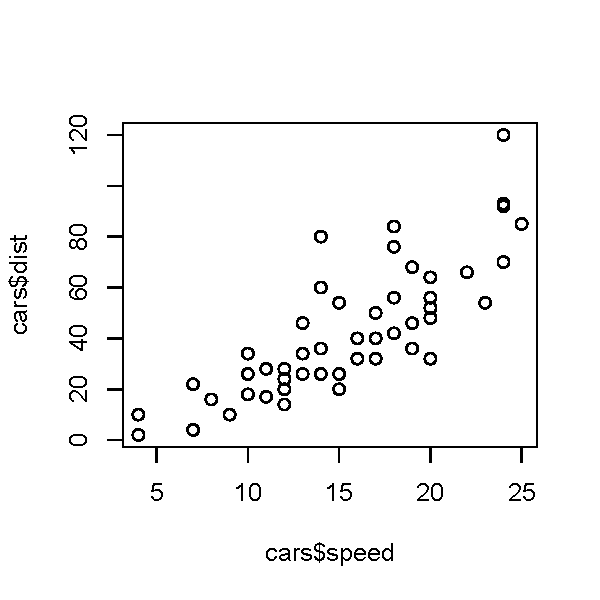
\includegraphics[width=.54\textwidth]{figure/pos-plot-1-1} 

}


\end{knitrout}

It is also possible, and usually more convenient, to use a \emph{formula} to specify the variables to be plotted on the $x$ and $y$ axes, passing additionally as an argument to  parameter \code{data} the name of the data frame containing these variables. The formula \code{dist \textasciitilde\ speed}, is read as \code{dist} explained by \code{speed}---i.e., \code{dist} is mapped to the $y$-axis as the dependent variable and \code{speed} to the $x$-axis as the independent variable.

\begin{knitrout}\footnotesize
\definecolor{shadecolor}{rgb}{0.969, 0.969, 0.969}\color{fgcolor}\begin{kframe}
\begin{alltt}
\hlkwd{plot}\hlstd{(dist} \hlopt{~} \hlstd{speed,} \hlkwc{data} \hlstd{= cars)}
\end{alltt}
\end{kframe}

{\centering 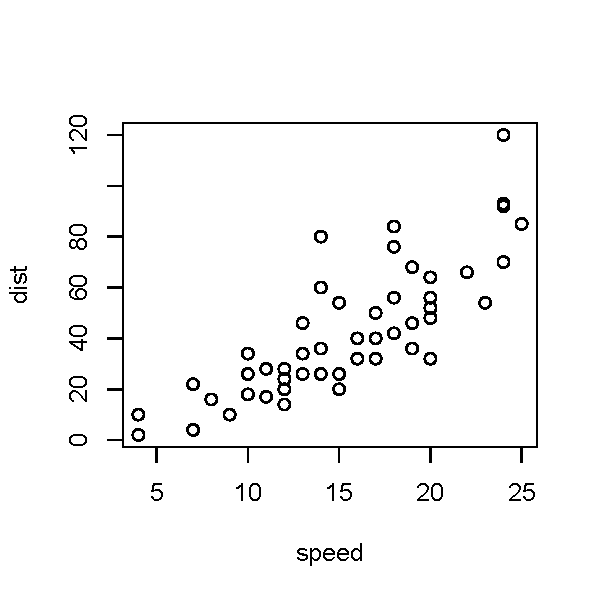
\includegraphics[width=.54\textwidth]{figure/pos-plot-2-1} 

}


\end{knitrout}

Within \Rlang there exist different specializations, or ``flavors,'' of method \Rfunction{plot()} that become active depending on the class of the variables passed as arguments: passing two numerical variables results in a scatter plot as seen above. In contrast passing one factor and one numeric variable to \code{plot()} results in a box-and-whiskers plot being produced. To exemplify this we need to use a different data set, here \code{chickwts} as \code{cars} does not contain any factors. Use \code{help("chickwts")} to learn more about this data set, also included in \Rpgrm .

\begin{knitrout}\footnotesize
\definecolor{shadecolor}{rgb}{0.969, 0.969, 0.969}\color{fgcolor}\begin{kframe}
\begin{alltt}
\hlkwd{plot}\hlstd{(weight} \hlopt{~} \hlstd{feed,} \hlkwc{data} \hlstd{= chickwts)}
\end{alltt}
\end{kframe}

{\centering 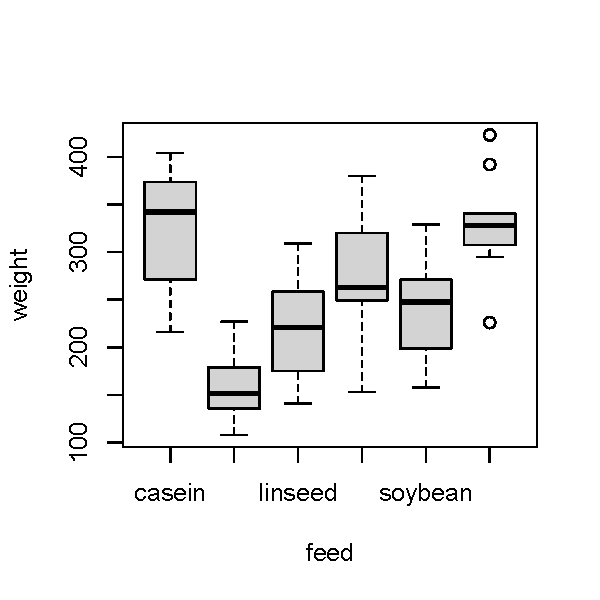
\includegraphics[width=.54\textwidth]{figure/pos-plot-3-1} 

}


\end{knitrout}

Method \Rfunction{plot()} and variants defined in \Rlang, when used for plotting return their graphical output to a \emph{graphical output device}.

When \Rlang is used interactively, a software device is opened automatically to output the graphical output to a physical device, usually the computer screen. The name of the \Rlang software device used may depend on the operating system (e.g.,  \osname{MS-Windows} or \osname{Linux}), or on the IDE (e.g., \RStudio).

In \Rlang, software graphical devices not necessarily generate output on a physical device like a printer, as several of these devices translate the plotting commands into a file format and save it to disk. Several different graphical devices are available in \Rlang and they differ in the kind of output they produce: raster files (e.g., TIFF, PNG and JPEG formats), vector graphics files (e.g., SVG, EPS and PDF), or output to a physical device like the screen of a computer. Additional devices are available through contributed \Rlang packages.

Devices follow the paradigm of ON and OFF switches, opening and closing a destination for \code{print()}, \code{plot()} and related functions. Some devices producing a file as output, can save their output one plot at a time to single-page graphic files or only when the device is closed, possibly as a multi-page file.

When opening a device the user supplies additional information. For the PDF device that produces output in a vector-graphics format, width and height of the output are specified in \emph{inches}. A default file name is used unless we pass a \code{character} string as an argument to parameter \code{file}.

\begin{knitrout}\footnotesize
\definecolor{shadecolor}{rgb}{0.969, 0.969, 0.969}\color{fgcolor}\begin{kframe}
\begin{alltt}
\hlkwd{pdf}\hlstd{(}\hlkwc{file} \hlstd{=} \hlstr{"output/my-file.pdf"}\hlstd{,} \hlkwc{width} \hlstd{=} \hlnum{6}\hlstd{,} \hlkwc{height} \hlstd{=} \hlnum{5}\hlstd{,} \hlkwc{onefile} \hlstd{=} \hlnum{TRUE}\hlstd{)}
\hlkwd{plot}\hlstd{(dist} \hlopt{~} \hlstd{speed,} \hlkwc{data} \hlstd{= cars)}
\hlkwd{plot}\hlstd{(weight} \hlopt{~} \hlstd{feed,} \hlkwc{data} \hlstd{= chickwts)}
\hlkwd{dev.off}\hlstd{()}
\end{alltt}
\begin{verbatim}
## cairo_pdf 
##         2
\end{verbatim}
\end{kframe}
\end{knitrout}

Raster devices return bitmaps and \code{width} and \code{height} are specified in \emph{pixels}.

\begin{knitrout}\footnotesize
\definecolor{shadecolor}{rgb}{0.969, 0.969, 0.969}\color{fgcolor}\begin{kframe}
\begin{alltt}
\hlkwd{png}\hlstd{(}\hlkwc{file} \hlstd{=} \hlstr{"output/my-file.png"}\hlstd{,} \hlkwc{width} \hlstd{=} \hlnum{600}\hlstd{,} \hlkwc{height} \hlstd{=} \hlnum{500}\hlstd{)}
\hlkwd{plot}\hlstd{(weight} \hlopt{~} \hlstd{feed,} \hlkwc{data} \hlstd{= chickwts)}
\hlkwd{dev.off}\hlstd{()}
\end{alltt}
\begin{verbatim}
## cairo_pdf 
##         2
\end{verbatim}
\end{kframe}
\end{knitrout}

The approach of direct output to a software device is used in base \Rlang,
and the addition of plot components, as shown below, is done directly to the output device.

\begin{knitrout}\footnotesize
\definecolor{shadecolor}{rgb}{0.969, 0.969, 0.969}\color{fgcolor}\begin{kframe}
\begin{alltt}
\hlkwd{png}\hlstd{(}\hlkwc{file} \hlstd{=} \hlstr{"output/my-file.png"}\hlstd{,} \hlkwc{width} \hlstd{=} \hlnum{600}\hlstd{,} \hlkwc{height} \hlstd{=} \hlnum{500}\hlstd{)}
\hlkwd{plot}\hlstd{(dist} \hlopt{~} \hlstd{speed,} \hlkwc{data} \hlstd{= cars)}
\hlkwd{text}\hlstd{(}\hlkwc{x} \hlstd{=} \hlnum{10}\hlstd{,} \hlkwc{y} \hlstd{=} \hlnum{110}\hlstd{,} \hlkwc{labels} \hlstd{=} \hlstr{"some texts to be added"}\hlstd{)}
\hlkwd{dev.off}\hlstd{()}
\end{alltt}
\begin{verbatim}
## cairo_pdf 
##         2
\end{verbatim}
\end{kframe}
\end{knitrout}

\begin{infobox}
This is not the only approach available. As we will see in chapter \ref{chap:R:plotting} starting on page \pageref{chap:R:plotting}, an alternative approach is to build a \emph{plot object} as a list of member components that is later rendered as a whole on a graphical device by calling \code{print()} once.
\end{infobox}

\section{Further reading}
For\index{further reading!using the R language} further reading on the aspects of \Rlang discussed in the current chapter,
 I suggest the books \citetitle{Peng2016} (\citeauthor{Peng2016}) and \citetitle{Matloff2011} (\citeauthor{Matloff2011}).



\index{data!exploration at the R console|)}
















\backmatter

\printbibliography

\printindex\label{idx:general}

\printindex[rcatsidx]\label{idx:rcats}

\printindex[rindex]\label{idx:rindex}

\end{document}

\appendix

\chapter{Build information}

\begin{knitrout}\footnotesize
\definecolor{shadecolor}{rgb}{0.969, 0.969, 0.969}\color{fgcolor}\begin{kframe}
\begin{alltt}
\hlkwd{Sys.info}\hlstd{()}
\end{alltt}
\end{kframe}
\end{knitrout}



\begin{knitrout}\footnotesize
\definecolor{shadecolor}{rgb}{0.969, 0.969, 0.969}\color{fgcolor}\begin{kframe}
\begin{alltt}
\hlkwd{sessionInfo}\hlstd{()}
\end{alltt}
\end{kframe}
\end{knitrout}

\end{document}


